\documentclass[11pt]{article}
\usepackage[margin=2cm]{geometry}
\usepackage{amsmath,amssymb}
\usepackage{graphicx}
\usepackage{booktabs}
\usepackage{array}
\usepackage{xcolor}
\usepackage[breakable]{tcolorbox}
\usepackage{enumitem}
\usepackage[hidelinks]{hyperref}
\allowdisplaybreaks
\setlength{\parindent}{0pt}
\setlength{\parskip}{4pt}
\definecolor{stepc}{HTML}{1F4E9E}
\definecolor{ansc}{HTML}{0B6E4F}
\newcommand{\solstep}[2]{\par\medskip{\color{stepc}\textbf{Step #1 --- #2}}\par\nopagebreak}
\newtcolorbox{probbox}[1]{colback=white,colframe=black!55,fonttitle=\bfseries,title={#1}}
\newtcolorbox{ansbox}{breakable,colback=ansc!6,colframe=ansc,fonttitle=\bfseries,title={Answer}}
\newtcolorbox{cardbox}[1]{breakable,colback=stepc!4,colframe=stepc,fonttitle=\bfseries,title={#1}}
\graphicspath{{../../../output/lecture2/2D_finite_gbw/}}
\title{Set 2D: Op-Amps with Finite Gain-Bandwidth}
\author{ECEN 325 --- Lecture 2 (Operational Amplifiers) practice set}
\date{}
\begin{document}
\maketitle

\textbf{What this set trains.} Real op-amps have a finite open-loop gain $A(s)=\frac{A_0}{1+s/\omega_b}$.
Instead of the virtual short you write $V_{out}=A(V_+-V_-)$, express $V_+$ and $V_-$ with dividers (superposition),
and solve. For resistive (or purely capacitive) feedback the result is always the ideal gain times a single pole
near $\beta\omega_t$: the gain-bandwidth trade-off. Problems 1--6 are easy, 7--12 medium, 13--18 hard. Try each
problem before looking at its solution.


\begin{cardbox}{The Lecture-2 pipeline (use it for every problem in this lecture)}
\textbf{Tools --- this is all the theory you need (plus the Lecture-1 tools for impedances, dividers, Bode plots
and sinusoids):}
\begin{enumerate}[label=\textbf{T\arabic*},leftmargin=2.2em,itemsep=1pt]
\item \emph{Ideal op-amp with negative feedback:} no current into $+$ or $-$; $V_-=V_+$ (virtual short).
      Its output is an ideal voltage source (loads on it do not matter).
\item \emph{Block formulas:} inverting $\frac{V_o}{V_{in}}=-\frac{Z_f}{Z_{in}}$; non-inverting
      $\frac{V_o}{V_+}=1+\frac{Z_f}{Z_g}$ (with $V_+$ from the divider at the $+$ input); a follower has gain 1.
      Several blocks in cascade: multiply.
\item \emph{KCL with impedances:} at a node, $\sum_k \frac{V_{node}-V_k}{Z_k}=0$ (for a capacitor
      $\frac{1}{Z}=sC$). Write it at every node except op-amp outputs and source nodes.
\item \emph{Solving KCL equations:} pick the equation with the fewest unknowns, solve it for one node voltage,
      substitute into the rest; repeat until only $V_o$ and $V_i$ remain.
\item \emph{Finite gain:} $V_{out}=A(s)(V_+-V_-)$, $A(s)=\frac{A_0}{1+s/\omega_b}$, $\omega_t=A_0\omega_b$.
      With $V_+=\alpha_+V_{in}$, $V_-=\alpha_-V_{in}+\beta V_{out}$: $\frac{V_{out}}{V_{in}}=\frac{A(\alpha_+-\alpha_-)}{1+A\beta}$.
\item \emph{Slew rate:} for $V_{out}=\hat V\sin\omega t$, the fastest change is $\left|\frac{dV_{out}}{dt}\right|_{max}=\omega\hat V$;
      no distortion requires $\omega\hat V\le SR$.
\end{enumerate}
\textbf{Steps:}
\begin{enumerate}[leftmargin=2.2em,itemsep=1pt]
\item \emph{Sources.} DC and AC both present $\Rightarrow$ superposition.
\item \emph{DC circuit:} $V_i\to0$, $C\to$ open; pass the DC through each block with its gain at $s=0$.
\item \emph{Op-amp rules:} confirm negative feedback; apply T1 (or T5 for a non-ideal op-amp).
\item \emph{Transfer function:} standard blocks $\to$ T2; anything else $\to$ T3 + T4.
\item \emph{Standard form}, \ 6.~\emph{Bode}, \ 7.~\emph{Output} --- exactly as in Lecture 1.
\end{enumerate}
\emph{Variations:} a design problem runs these steps backwards (Bode plot $\to H(s)\to$ blocks $\to$ component values);
a slew-rate problem stops after Step 4 for every op-amp output and applies T6.
\end{cardbox}

\section*{Problems}
\subsection*{Easy problems}
\begin{probbox}{Problem 2D.1 \hfill Easy}
For the circuit below, where every op-amp has the open-loop gain $A(s)=\dfrac{10^{5}}{1+\dfrac{s}{2\pi\cdot 10}}$: (a) find $H(s)=\dfrac{V_o(s)}{V_i(s)}$ and sketch its magnitude Bode plot; (b) find the steady-state output $V_o(t)$ for $V_i(t) = 0.1\sin\left(2\pi\cdot 50000\,t\right)$.
\begin{center}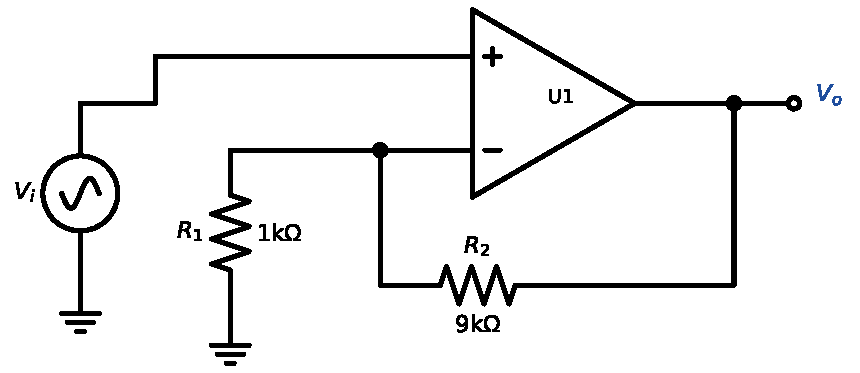
\includegraphics[width=\linewidth,height=5.6cm,keepaspectratio]{p01_circuit}\end{center}
\end{probbox}

\begin{probbox}{Problem 2D.2 \hfill Easy}
For the circuit below, where every op-amp has the open-loop gain $A(s)=\dfrac{2\times 10^{5}}{1+\dfrac{s}{2\pi\cdot 5}}$: (a) find $H(s)=\dfrac{V_o(s)}{V_i(s)}$ and sketch its magnitude Bode plot; (b) find the steady-state output $V_o(t)$ for $V_i(t) = 0.2\sin\left(2\pi\cdot 10^{5}\,t\right)$.
\begin{center}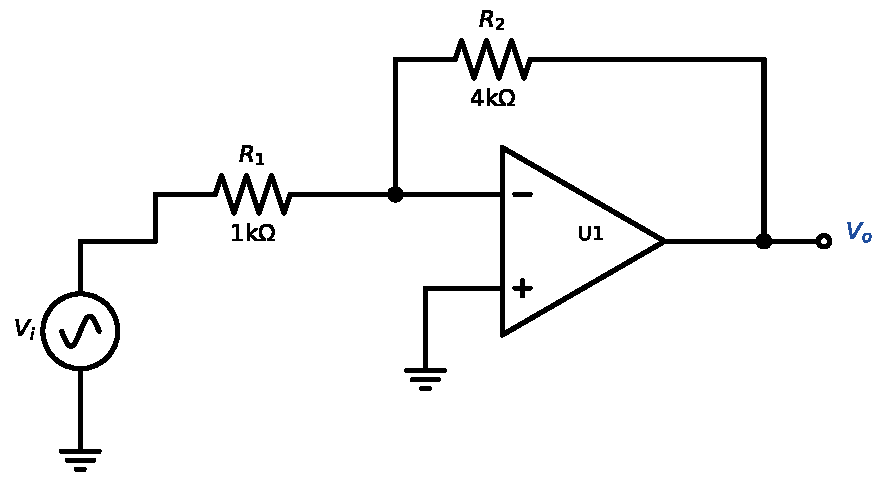
\includegraphics[width=\linewidth,height=5.6cm,keepaspectratio]{p02_circuit}\end{center}
\end{probbox}

\begin{probbox}{Problem 2D.3 \hfill Easy}
For the circuit below, where every op-amp has the open-loop gain $A(s)=\dfrac{10^{5}}{1+\dfrac{s}{2\pi\cdot 20}}$: (a) find $H(s)=\dfrac{V_o(s)}{V_i(s)}$ and sketch its magnitude Bode plot; (b) find the steady-state output $V_o(t)$ for $V_i(t) = 1\sin\left(2\pi\cdot 5\times 10^{5}\,t\right)$.
\begin{center}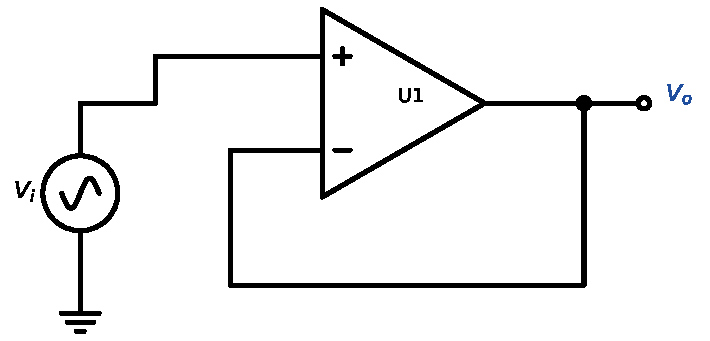
\includegraphics[width=\linewidth,height=5.6cm,keepaspectratio]{p03_circuit}\end{center}
\end{probbox}

\begin{probbox}{Problem 2D.4 \hfill Easy}
For the circuit below, where every op-amp has the open-loop gain $A(s)=\dfrac{10^{5}}{1+\dfrac{s}{2\pi\cdot 10}}$: (a) find $H(s)=\dfrac{V_o(s)}{V_i(s)}$ and sketch its magnitude Bode plot; (b) find the steady-state output $V_o(t)$ for $V_i(t) = 0.2\sin\left(2\pi\cdot 20000\,t\right)$.
\begin{center}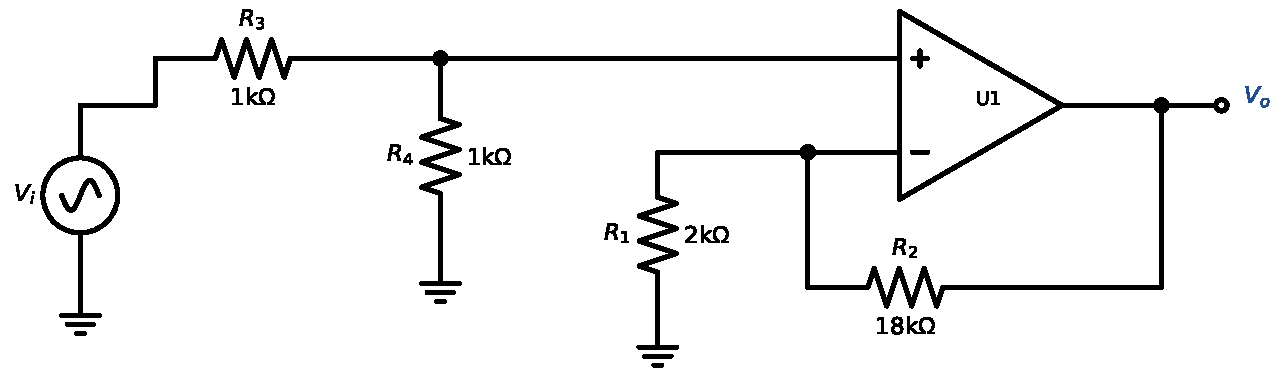
\includegraphics[width=\linewidth,height=5.6cm,keepaspectratio]{p04_circuit}\end{center}
\end{probbox}

\begin{probbox}{Problem 2D.5 \hfill Easy}
For the circuit below, where every op-amp has the open-loop gain $A(s)=\dfrac{10^{5}}{1+\dfrac{s}{2\pi\cdot 10}}$: (a) find $H(s)=\dfrac{V_o(s)}{V_i(s)}$ and sketch its magnitude Bode plot; (b) find the steady-state output $V_o(t)$ for $V_i(t) = 0.05\sin\left(2\pi\cdot 50000\,t\right)$.
\begin{center}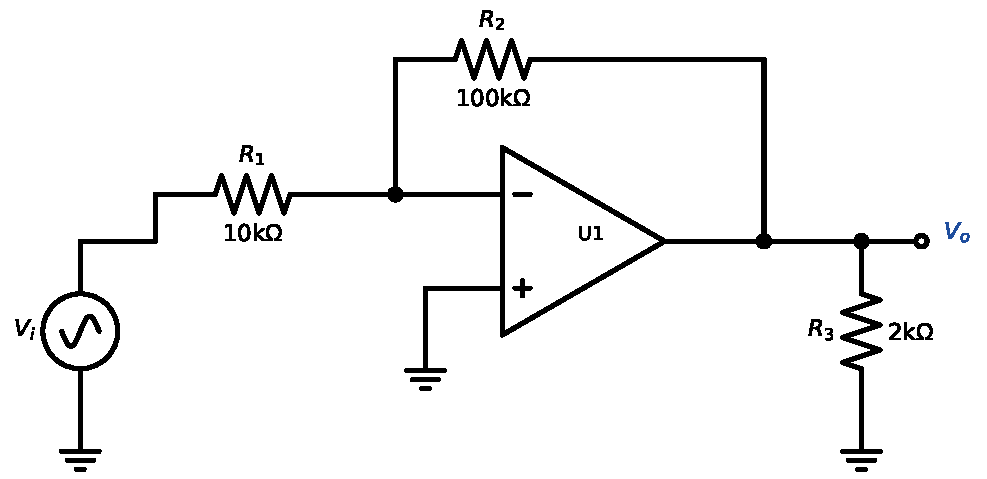
\includegraphics[width=\linewidth,height=5.6cm,keepaspectratio]{p05_circuit}\end{center}
\end{probbox}

\begin{probbox}{Problem 2D.6 \hfill Easy}
For the circuit below, where every op-amp has the open-loop gain $A(s)=\dfrac{10^{5}}{1+\dfrac{s}{2\pi\cdot 10}}$: (a) find $H(s)=\dfrac{V_o(s)}{V_i(s)}$ and sketch its magnitude Bode plot; (b) find the steady-state output $V_o(t)$ for $V_i(t) = 0.2\sin\left(2\pi\cdot 2\times 10^{5}\,t\right)$.
\begin{center}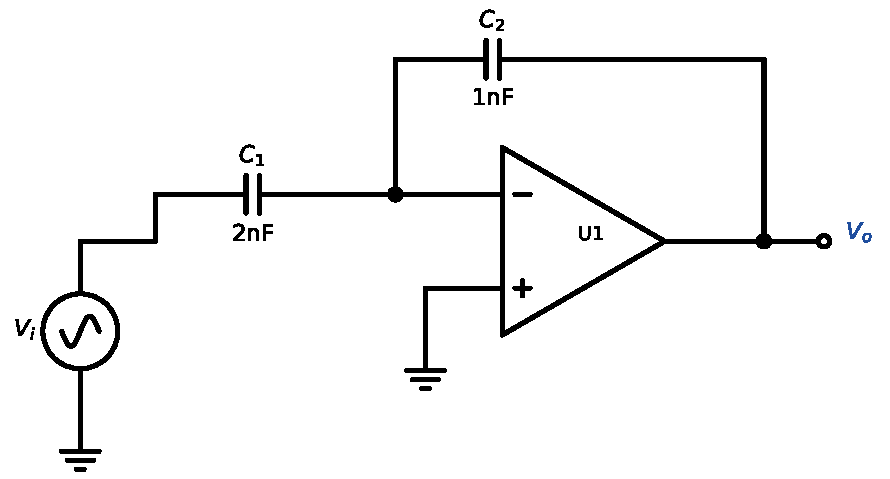
\includegraphics[width=\linewidth,height=5.6cm,keepaspectratio]{p06_circuit}\end{center}
\end{probbox}

\subsection*{Medium problems}
\begin{probbox}{Problem 2D.7 \hfill Medium}
For the circuit below, where every op-amp has the open-loop gain $A(s)=\dfrac{10^{5}}{1+\dfrac{s}{2\pi\cdot 20}}$: (a) find $H(s)=\dfrac{V_o(s)}{V_i(s)}$ and sketch its magnitude Bode plot; (b) find the steady-state output $V_o(t)$ for $V_i(t) = 0.01\sin\left(2\pi\cdot 10^{5}\,t\right)$.
\begin{center}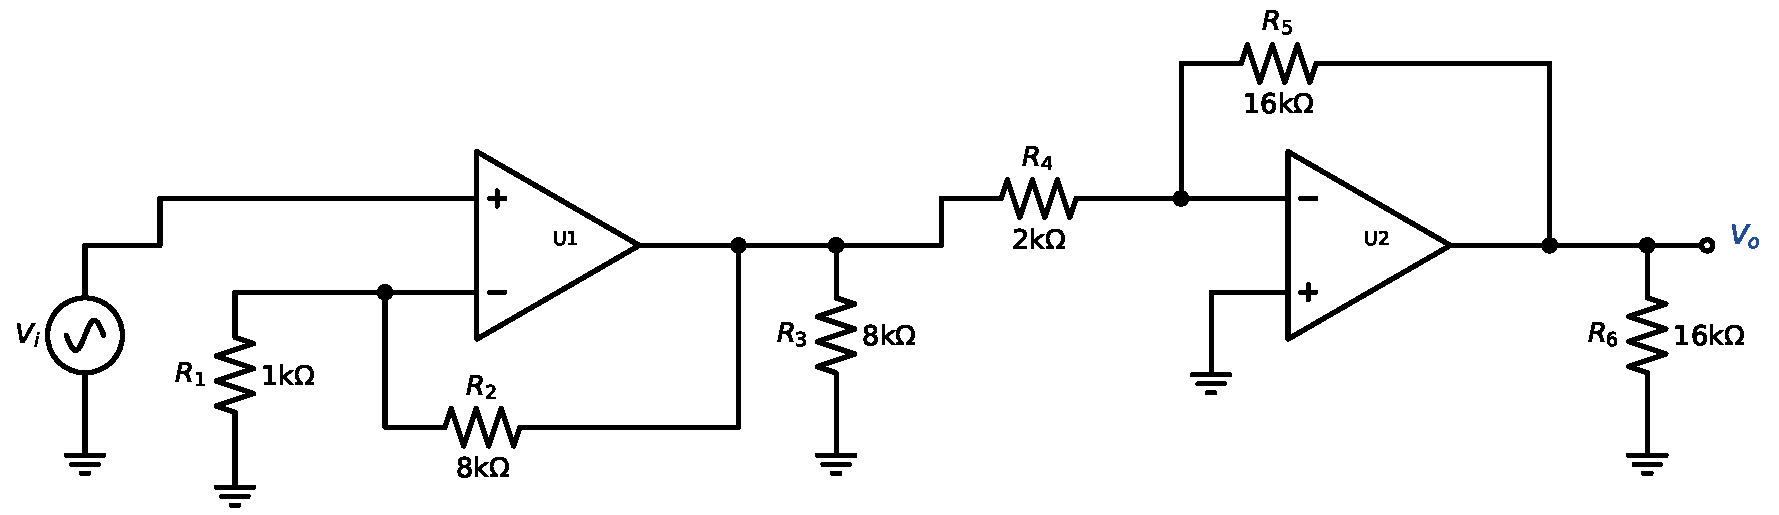
\includegraphics[width=\linewidth,height=5.6cm,keepaspectratio]{p07_circuit}\end{center}
\end{probbox}

\begin{probbox}{Problem 2D.8 \hfill Medium}
For the circuit below, where every op-amp has the open-loop gain $A(s)=\dfrac{10^{5}}{1+\dfrac{s}{2\pi\cdot 10}}$: (a) find $H(s)=\dfrac{V_o(s)}{V_i(s)}$ and sketch its magnitude Bode plot; (b) find the steady-state output $V_o(t)$ for $V_i(t) = 0.1\sin\left(2\pi\cdot 20000\,t\right)$.
\begin{center}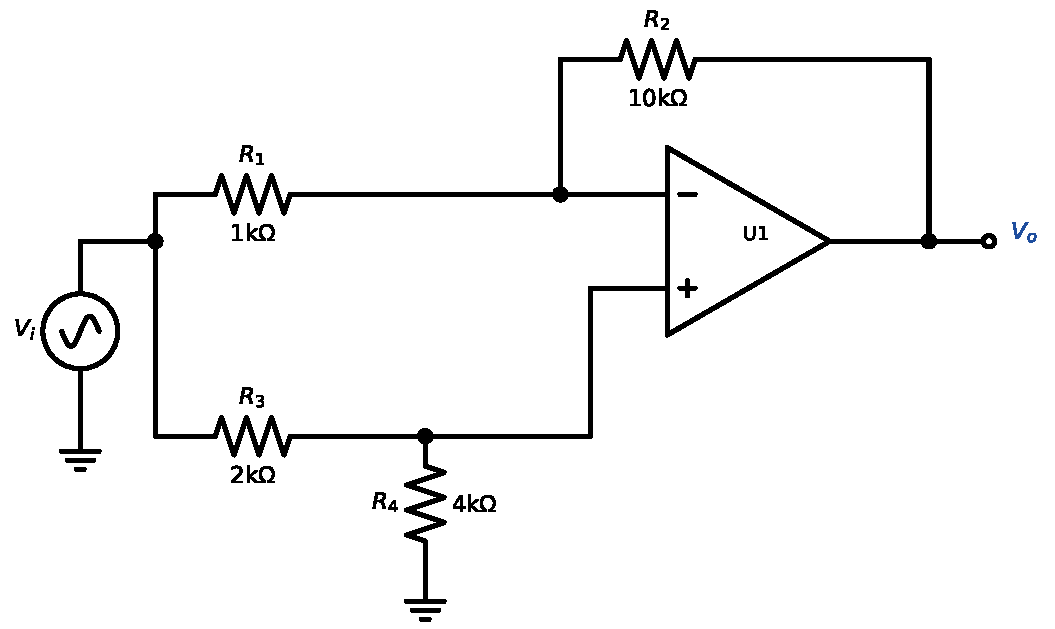
\includegraphics[width=\linewidth,height=5.6cm,keepaspectratio]{p08_circuit}\end{center}
\end{probbox}

\begin{probbox}{Problem 2D.9 \hfill Medium}
For the circuit below, where every op-amp has the open-loop gain $A(s)=\dfrac{10^{5}}{1+\dfrac{s}{2\pi\cdot 10}}$: (a) find $H(s)=\dfrac{V_o(s)}{V_i(s)}$ and sketch its magnitude Bode plot; (b) find the steady-state output $V_o(t)$ for $V_i(t) = 0.01\sin\left(2\pi\cdot 50000\,t\right)$.
\begin{center}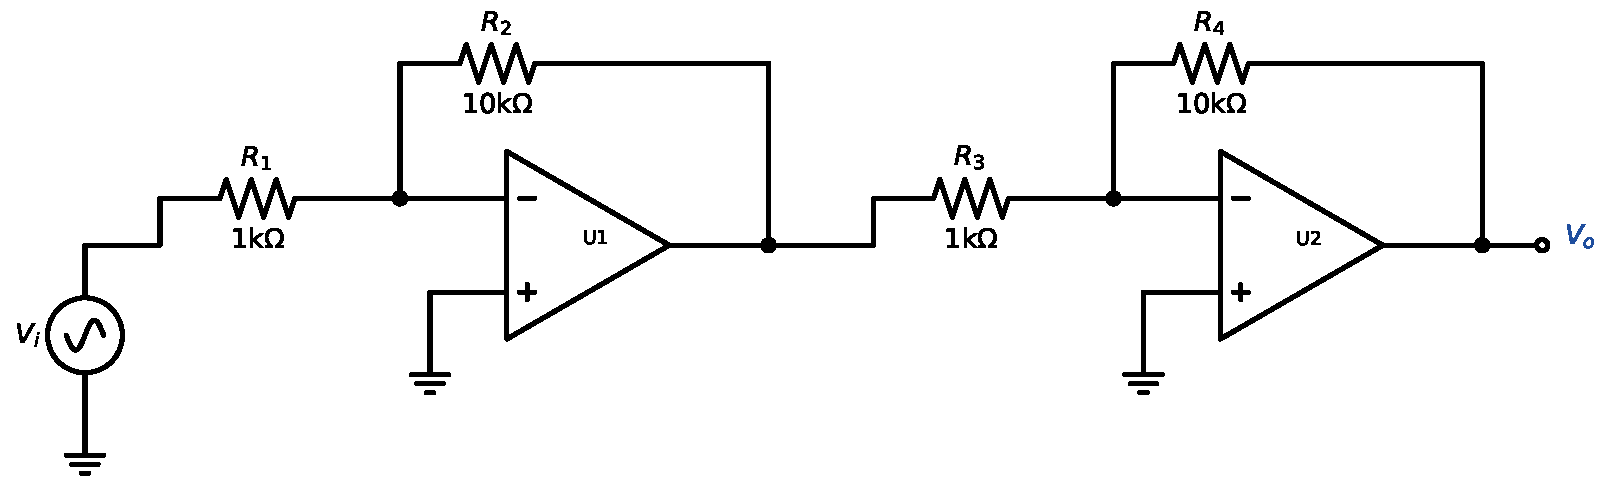
\includegraphics[width=\linewidth,height=5.6cm,keepaspectratio]{p09_circuit}\end{center}
\end{probbox}

\begin{probbox}{Problem 2D.10 \hfill Medium}
For the circuit below, where every op-amp has the open-loop gain $A(s)=\dfrac{10^{5}}{1+\dfrac{s}{2\pi\cdot 30}}$: (a) find $H(s)=\dfrac{V_o(s)}{V_i(s)}$ and sketch its magnitude Bode plot; (b) find the steady-state output $V_o(t)$ for $V_i(t) = 0.05\sin\left(2\pi\cdot 5\times 10^{5}\,t\right)$.
\begin{center}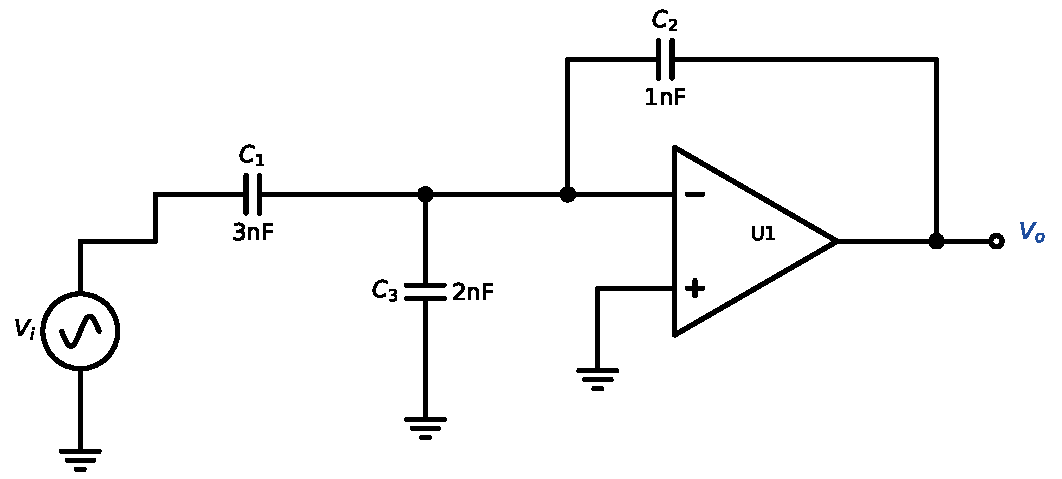
\includegraphics[width=\linewidth,height=5.6cm,keepaspectratio]{p10_circuit}\end{center}
\end{probbox}

\begin{probbox}{Problem 2D.11 \hfill Medium}
For the circuit below, where every op-amp has the open-loop gain $A(s)=\dfrac{10^{5}}{1+\dfrac{s}{2\pi\cdot 10}}$: (a) find $H(s)=\dfrac{V_o(s)}{V_i(s)}$ and sketch its magnitude Bode plot; (b) find the steady-state output $V_o(t)$ for $V_i(t) = 0.01\sin\left(2\pi\cdot 5000\,t\right)$.
\begin{center}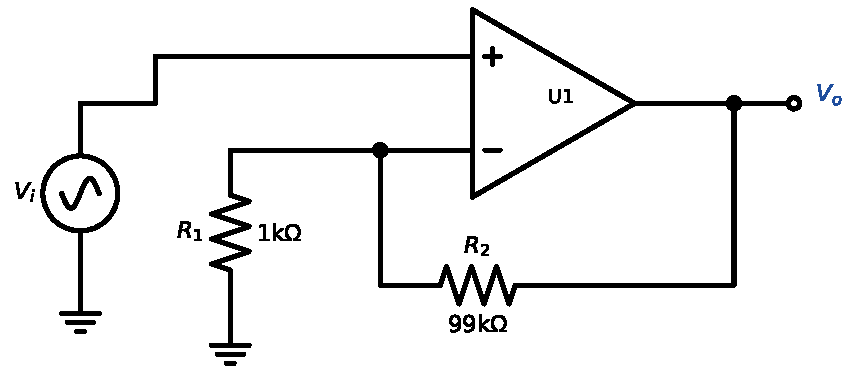
\includegraphics[width=\linewidth,height=5.6cm,keepaspectratio]{p11_circuit}\end{center}
\end{probbox}

\begin{probbox}{Problem 2D.12 \hfill Medium}
For the circuit below, where every op-amp has the open-loop gain $A(s)=\dfrac{2\times 10^{5}}{1+\dfrac{s}{2\pi\cdot 5}}$: (a) find $H(s)=\dfrac{V_o(s)}{V_i(s)}$ and sketch its magnitude Bode plot; (b) find the steady-state output $V_o(t)$ for $V_i(t) = 0.1\sin\left(2\pi\cdot 2\times 10^{5}\,t\right)$.
\begin{center}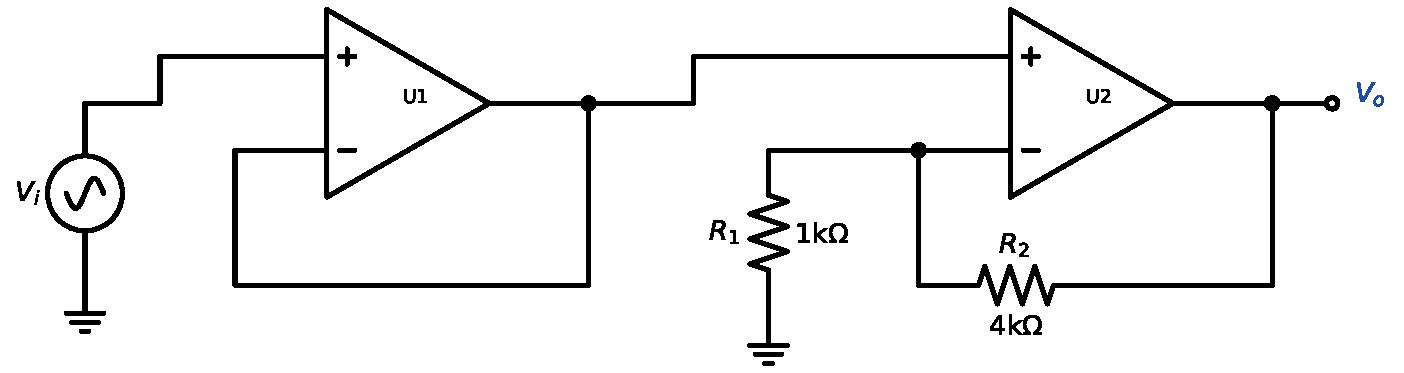
\includegraphics[width=\linewidth,height=5.6cm,keepaspectratio]{p12_circuit}\end{center}
\end{probbox}

\subsection*{Hard problems}
\begin{probbox}{Problem 2D.13 \hfill Hard}
For the circuit below, where every op-amp has the open-loop gain $A(s)=\dfrac{10^{5}}{1+\dfrac{s}{2\pi\cdot 10}}$: (a) find $H(s)=\dfrac{V_o(s)}{V_i(s)}$ and sketch its magnitude Bode plot; (b) find the steady-state output $V_o(t)$ for $V_i(t) = 0.02\sin\left(2\pi\cdot 10^{5}\,t\right)$.
\begin{center}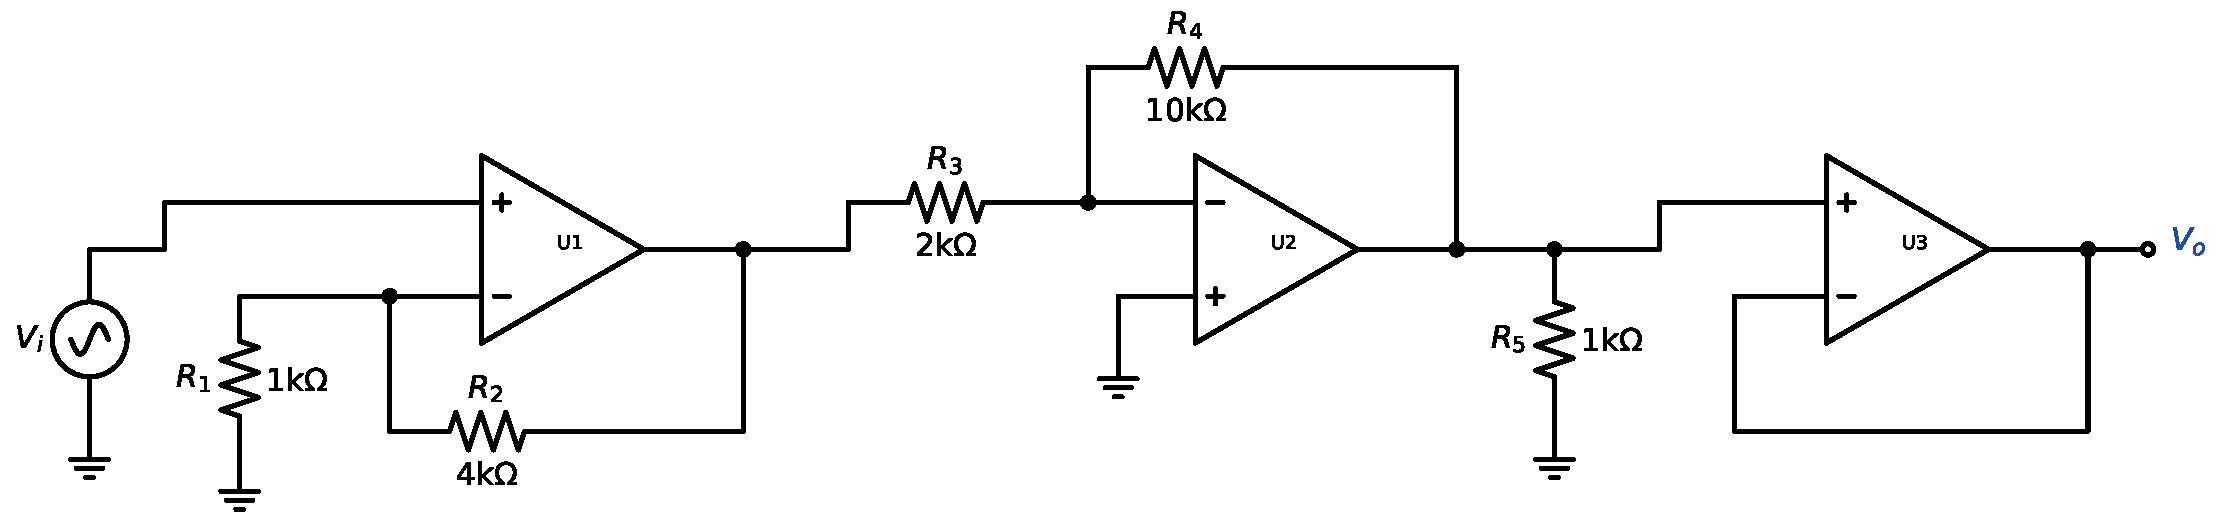
\includegraphics[width=\linewidth,height=5.6cm,keepaspectratio]{p13_circuit}\end{center}
\end{probbox}

\begin{probbox}{Problem 2D.14 \hfill Hard}
For the circuit below, where every op-amp has the open-loop gain $A(s)=\dfrac{10^{5}}{1+\dfrac{s}{2\pi\cdot 20}}$: (a) find $H(s)=\dfrac{V_o(s)}{V_i(s)}$ and sketch its magnitude Bode plot; (b) find the steady-state output $V_o(t)$ for $V_i(t) = 0.05\sin\left(2\pi\cdot 50000\,t+\frac{\pi}{4}\right)$.
\begin{center}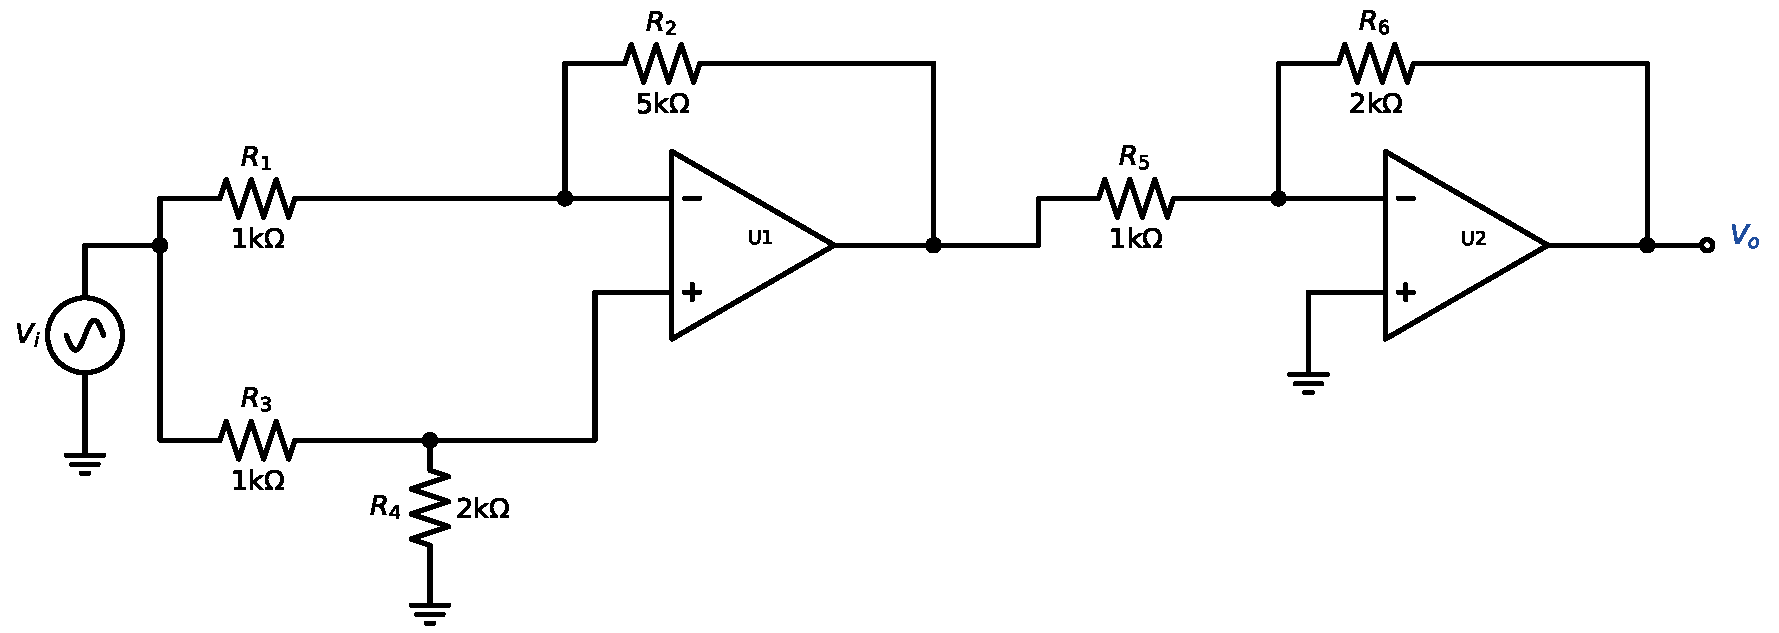
\includegraphics[width=\linewidth,height=5.6cm,keepaspectratio]{p14_circuit}\end{center}
\end{probbox}

\begin{probbox}{Problem 2D.15 \hfill Hard}
For the circuit below, where every op-amp has the open-loop gain $A(s)=\dfrac{10^{5}}{1+\dfrac{s}{2\pi\cdot 10}}$: (a) find $H(s)=\dfrac{V_o(s)}{V_i(s)}$ and sketch its magnitude Bode plot; (b) find the steady-state output $V_o(t)$ for $V_i(t) = 0.05\cos\left(2\pi\cdot 20000\,t\right)$.
\begin{center}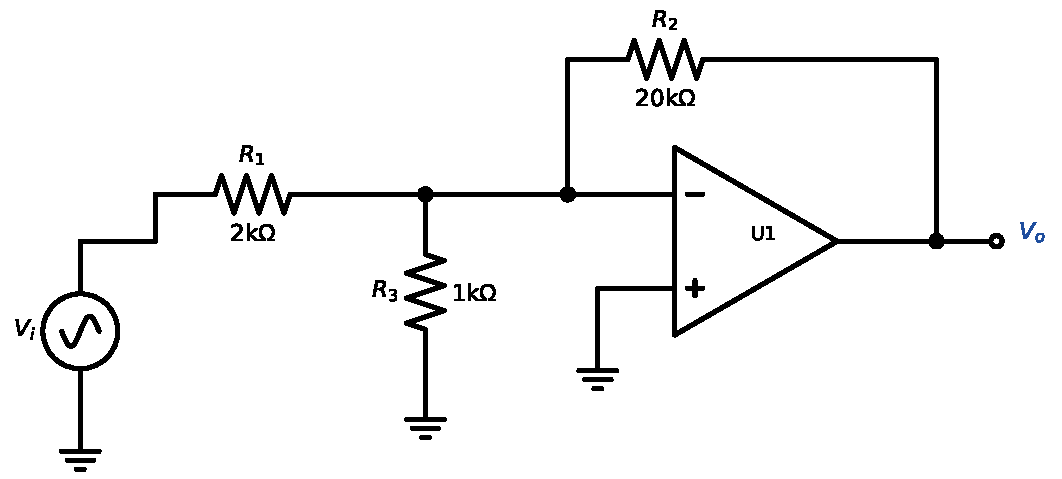
\includegraphics[width=\linewidth,height=5.6cm,keepaspectratio]{p15_circuit}\end{center}
\end{probbox}

\begin{probbox}{Problem 2D.16 \hfill Hard}
For the circuit below, where every op-amp has the open-loop gain $A(s)=\dfrac{10^{5}}{1+\dfrac{s}{2\pi\cdot 10}}$: (a) find $H(s)=\dfrac{V_o(s)}{V_i(s)}$ and sketch its magnitude Bode plot; (b) find the steady-state output $V_o(t)$ for $V_i(t) = 0.1\sin\left(2\pi\cdot 10000\,t\right)$.
\begin{center}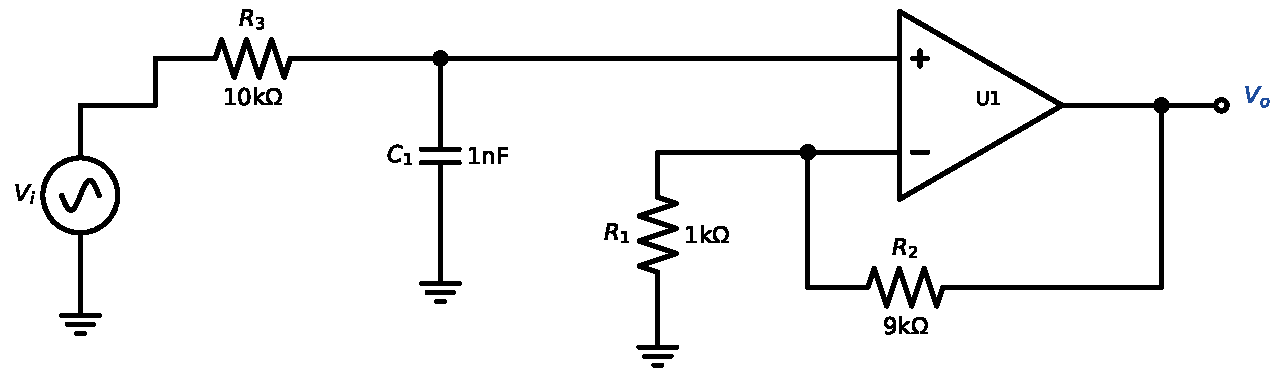
\includegraphics[width=\linewidth,height=5.6cm,keepaspectratio]{p16_circuit}\end{center}
\end{probbox}

\begin{probbox}{Problem 2D.17 \hfill Hard}
For the circuit below, where every op-amp has the open-loop gain $A(s)=\dfrac{10^{5}}{1+\dfrac{s}{2\pi\cdot 10}}$: (a) find $H(s)=\dfrac{V_o(s)}{V_i(s)}$ and sketch its magnitude Bode plot; (b) find the steady-state output $V_o(t)$ for $V_i(t) = 0.1\sin\left(2\pi\cdot 30000\,t-\frac{\pi}{6}\right)$.
\begin{center}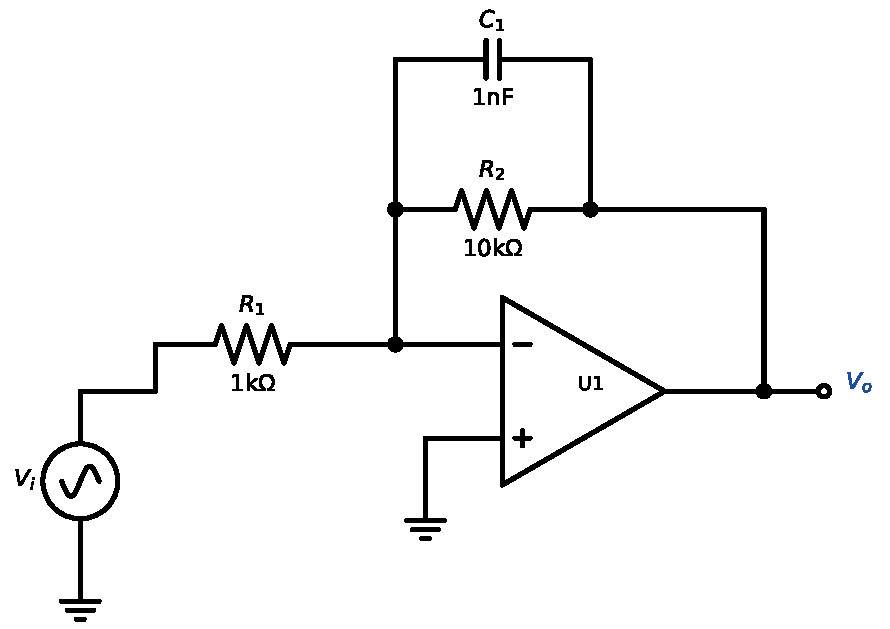
\includegraphics[width=\linewidth,height=5.6cm,keepaspectratio]{p17_circuit}\end{center}
\end{probbox}

\begin{probbox}{Problem 2D.18 \hfill Hard}
For the circuit below, where every op-amp has the open-loop gain $A(s)=\dfrac{10^{5}}{1+\dfrac{s}{2\pi\cdot 10}}$: (a) find $H(s)=\dfrac{V_o(s)}{V_i(s)}$ and sketch its magnitude Bode plot; (b) find the steady-state output $V_o(t)$ for $V_i(t) = 0.02\sin\left(2\pi\cdot 10^{5}\,t\right)$.
\begin{center}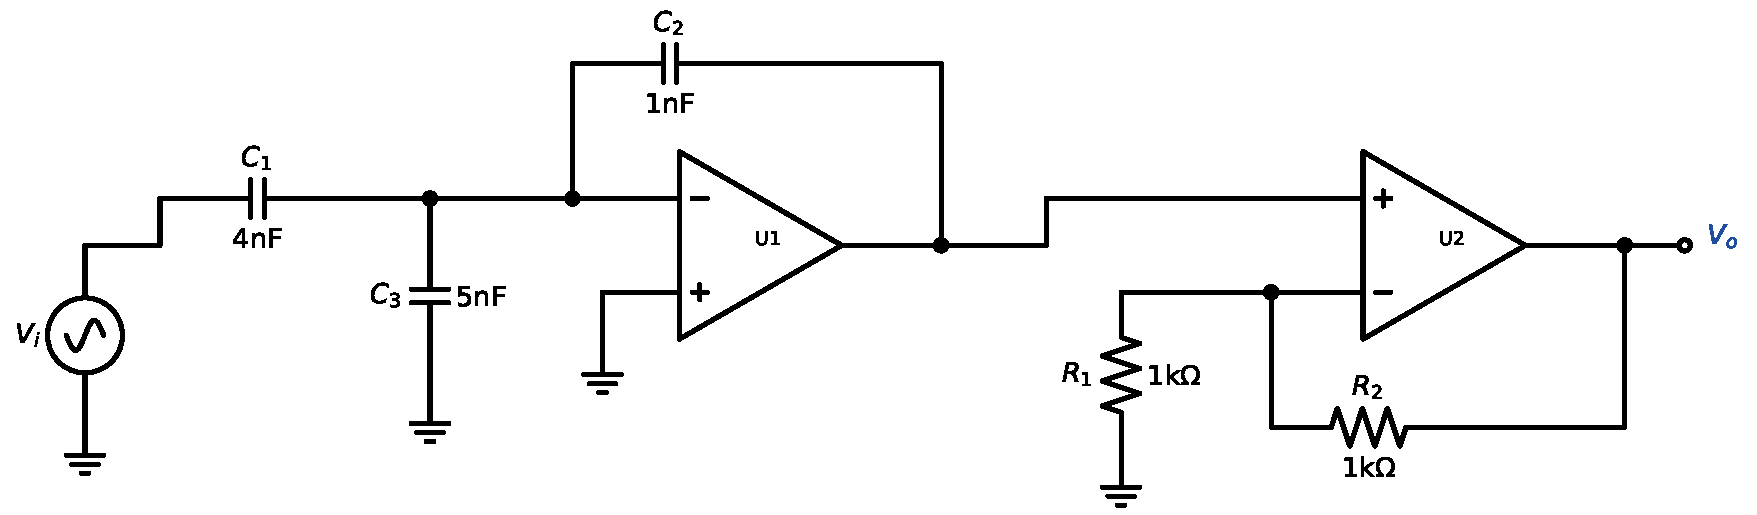
\includegraphics[width=\linewidth,height=5.6cm,keepaspectratio]{p18_circuit}\end{center}
\end{probbox}

\newpage
\section*{Solutions}
Every solution follows the steps of the Lecture-2 pipeline card.
\newpage
\subsection*{Solution 2D.1 \hfill Easy}
\begin{center}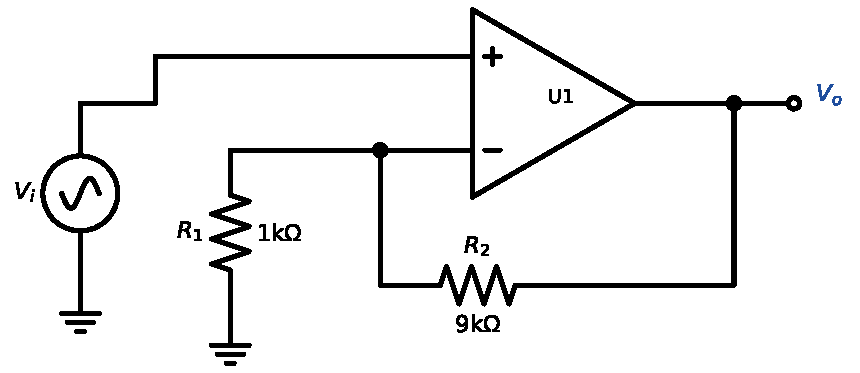
\includegraphics[width=\linewidth,height=5cm,keepaspectratio]{p01_circuit}\end{center}
\solstep{1}{Identify the sources}Independent sources: the AC input $V_i(t)$. No DC source: $V_{o,dc}=0$ and Step 2 is skipped.
\solstep{2}{DC circuit}No DC sources: $V_{o,dc}=0$.
\solstep{3}{Op-amp model}Non-ideal op-amp model (tool T5): $V_{out} = A(s)\,(V_+-V_-)$ with $A(s)=\dfrac{A_0}{1+s/\omega_b}$, $A_0=10^{5}$, $\omega_b = 2\pi\cdot10 = 62.8$\,rad/s, so the unity-gain frequency is $\omega_t = A_0\omega_b = 6.28\times 10^{6}$\,rad/s. The virtual short is \emph{not} used; only ``no current into the inputs'' is still true.

\solstep{4}{Transfer function, op-amp by op-amp}Recipe for each op-amp: write $V_+$ and $V_-$ by superposition of the block input and the op-amp output (each alone is a plain divider): $V_+ = \alpha_+V_{in}$, $V_- = \alpha_-V_{in}+\beta V_{out}$. Then $V_{out} = A(\alpha_+-\alpha_-)V_{in} - A\beta V_{out}$, i.e.\[
\frac{V_{out}}{V_{in}} = \frac{A(\alpha_+-\alpha_-)}{1+A\beta} = \frac{G}{1+\dfrac{1}{A\beta}},\qquad G = \frac{\alpha_+-\alpha_-}{\beta}\ \text{(the ideal gain)}
\]
With $A(s)$ inserted and constant $\alpha,\beta$:\[
\frac{V_{out}}{V_{in}} = G\,\frac{A_0\beta}{1+A_0\beta}\cdot\frac{1}{1+\dfrac{s}{\omega_b(1+A_0\beta)}},\qquad \omega_b(1+A_0\beta)\approx\beta\,\omega_t
\]

\textbf{Block 1 (U1).} (no current enters either input, so both are plain dividers)\begin{align*}
V_+ &= V_{i} \\
V_- &= \frac{R_{1}}{R_{1}+R_{2}}V_{o}
\end{align*}
So $\alpha_+ = 1$, $\alpha_- = 0$, $\beta = 0.1$: ideal gain $G = \frac{\alpha_+-\alpha_-}{\beta} = 10$, $A_0\beta = 10000$.\[
\frac{V_{o}}{V_{i}} = 10\cdot\frac{10000}{1+10000}\cdot\frac{1}{1+\dfrac{s}{6.28\times 10^{5}}} = \frac{9.999}{1+\dfrac{s}{6.28\times 10^{5}}}
\]
(closed-loop bandwidth $\omega_b(1+A_0\beta) = 6.28\times 10^{5}$\,rad/s, $f = 100 kHz$; compare $\beta\omega_t = 6.28\times 10^{5}$\,rad/s.)
So:\[
H(s) = \dfrac{6.28\times 10^{6}}{s + 6.28\times 10^{5}}
\]

\solstep{5}{Standard (Bode-ready) form}Find the roots. Every root $s=-p$ of the denominator is a \emph{pole}, every root $s=-z$ of the numerator is a \emph{zero}; $|p|$ and $|z|$ are the corner frequencies (rad/s).
\begin{itemize}[leftmargin=*,itemsep=2pt]
\item Denominator: $s + 6.28\times 10^{5}$; $s + 6.28\times 10^{5} = 0 \Rightarrow s = -6.28\times 10^{5}$.
\end{itemize}

Factored form (leading coefficient in front):
\[
H(s) = 6.28\times 10^{6}\,\dfrac{1}{(s+6.28\times 10^{5})}
\]

Bode-ready form: rewrite every $(s+p) = p\left(1+\frac{s}{p}\right)$ and $(s+z) = z\left(1+\frac{s}{z}\right)$, and collect all constants into $K$. Then every factor except $K$ is $\approx 1$ inside the pass-band:
\[
H(s) = 10\,\dfrac{1}{1+\dfrac{s}{2\pi\cdot 100\mathrm{k}}},\qquad K = 10
\]

\begin{center}\renewcommand{\arraystretch}{1.35}
\begin{tabular}{cccc}
\toprule
type & $\omega_c$ (rad/s) & $f_c=\omega_c/2\pi$ & slope change \\
\midrule
pole & $6.28\times 10^{5}$ & 100 kHz & $-20$ dB/dec \\
\bottomrule
\end{tabular}\end{center}

\solstep{6}{Magnitude Bode plot}Below every corner, all factors are $\approx$ constant: $|H| \approx 10$ $= 20$\,dB (flat, 0 dB/dec). Then, moving right, each pole bends the line down by 20\,dB/dec and each zero bends it up by 20\,dB/dec (tool T6):
\begin{center}\renewcommand{\arraystretch}{1.35}
\begin{tabular}{lcl}
\toprule
frequency range & slope & asymptote level \\
\midrule
$f<$ 100 kHz & $0$ dB/dec (flat) & 20 dB at end \\
$f>$ 100 kHz & $-20$ dB/dec & 20 dB at start \\
\bottomrule
\end{tabular}\end{center}

The flat (pass-band) level is $20\log_{10}|K| = 20\log_{10}10 = 20$\,dB.
\begin{center}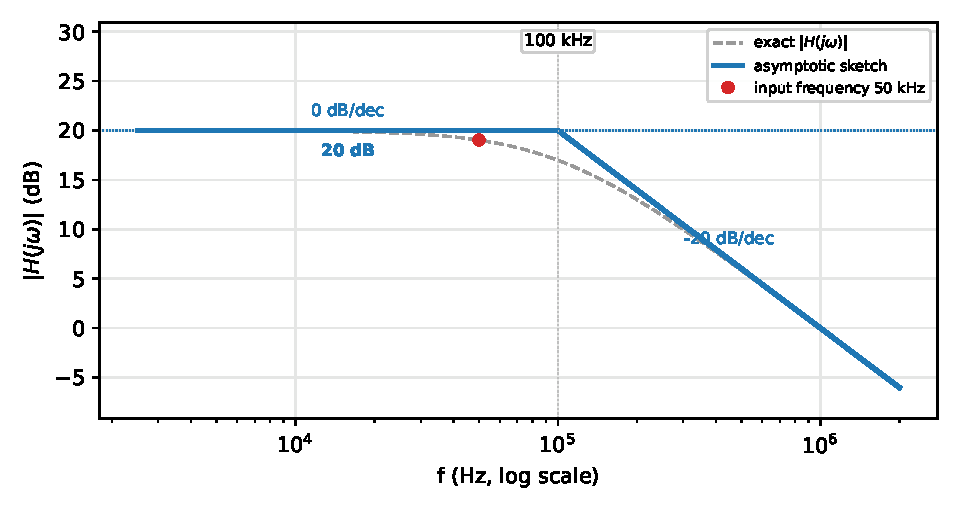
\includegraphics[width=0.78\linewidth,height=6.5cm,keepaspectratio]{p01_bode}\end{center}

{\small Blue: the straight-line sketch you are expected to draw. Dashed grey: the exact curve (about 3\,dB below the corner of an isolated pole). Red dot: the input frequency of Step 7.}
\solstep{7}{Steady-state output}The input is $V_i(t) = 0.1\sin\left(2\pi\cdot 50000\,t\right)$, so $\omega_{in} = 2\pi\cdot 50000 = 3.14\times 10^{5}$\,rad/s. Put $s=j\omega_{in}$ in each factor (tool T5): magnitudes multiply, angles add.
{\small Rules: $\left|\frac{s}{s+p}\right| = \frac{\omega}{\sqrt{\omega^2+p^2}}$, $\angle = \frac{\pi}{2}-\tan^{-1}\frac{\omega}{p}$;\quad $\left|\frac{1}{1+s/p}\right| = \frac{1}{\sqrt{1+(\omega/p)^2}}$, $\angle = -\tan^{-1}\frac{\omega}{p}$;\quad $\left|1+\frac{s}{z}\right| = \sqrt{1+(\omega/z)^2}$, $\angle = \tan^{-1}\frac{\omega}{z}$;\quad a negative $K$ adds $-\pi$.}
\begin{center}\renewcommand{\arraystretch}{1.35}
\begin{tabular}{ccc}
\toprule
factor & magnitude & angle (rad) \\
\midrule
$10$ & $9.999$ & $0$ \\
$\rule[-1.7em]{0pt}{4em}\dfrac{1}{1+\dfrac{s}{2\pi\cdot 100\mathrm{k}}}$ & $0.8944$ & $-0.464$ \\
\textbf{total} & $\mathbf{8.944}$ (product) & $\mathbf{-0.464}$ (sum) \\
\bottomrule
\end{tabular}\end{center}

\begin{align*}
|H(j\omega_{in})| &= 8.94, \qquad \angle H(j\omega_{in}) = -0.464\ \mathrm{rad} \\
v_{o,ac}(t) &= 8.94\times 0.1\,\sin\left(2\pi\cdot 50000\,t - 0.464\right) = 0.894\,\sin\left(2\pi\cdot 50000\,t - 0.464\right)
\end{align*}

\[
\boxed{V_o(t) = 0.894\,\sin\left(2\pi\cdot 50000\,t - 0.464\right)\ \mathrm{V}}
\]

\begin{ansbox}
$H(s) = 10\,\dfrac{1}{1+\dfrac{s}{2\pi\cdot 100\mathrm{k}}}$\quad (corners: 100 kHz)\\[4pt]
$V_o(t) = 0.894\,\sin\left(2\pi\cdot 50000\,t - 0.464\right)\ \mathrm{V}$
\end{ansbox}

\newpage
\subsection*{Solution 2D.2 \hfill Easy}
\begin{center}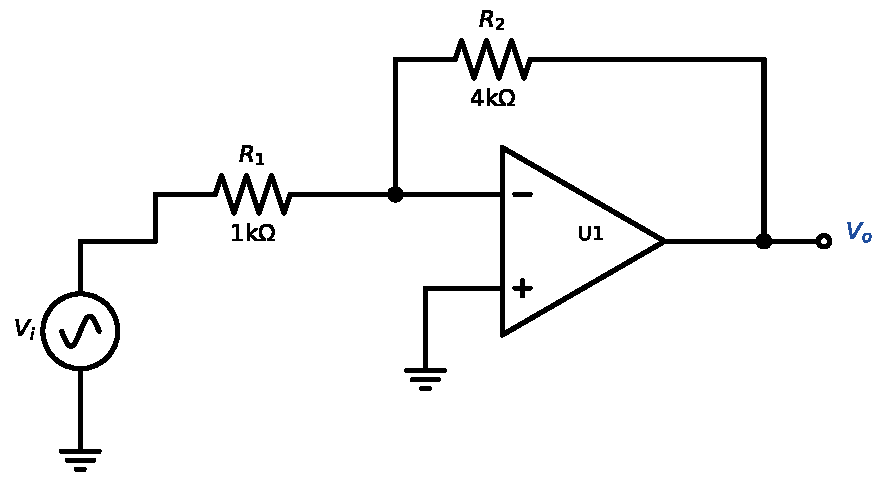
\includegraphics[width=\linewidth,height=5cm,keepaspectratio]{p02_circuit}\end{center}
\solstep{1}{Identify the sources}Independent sources: the AC input $V_i(t)$. No DC source: $V_{o,dc}=0$ and Step 2 is skipped.
\solstep{2}{DC circuit}No DC sources: $V_{o,dc}=0$.
\solstep{3}{Op-amp model}Non-ideal op-amp model (tool T5): $V_{out} = A(s)\,(V_+-V_-)$ with $A(s)=\dfrac{A_0}{1+s/\omega_b}$, $A_0=2\times 10^{5}$, $\omega_b = 2\pi\cdot5 = 31.4$\,rad/s, so the unity-gain frequency is $\omega_t = A_0\omega_b = 6.28\times 10^{6}$\,rad/s. The virtual short is \emph{not} used; only ``no current into the inputs'' is still true.

\solstep{4}{Transfer function, op-amp by op-amp}Recipe for each op-amp: write $V_+$ and $V_-$ by superposition of the block input and the op-amp output (each alone is a plain divider): $V_+ = \alpha_+V_{in}$, $V_- = \alpha_-V_{in}+\beta V_{out}$. Then $V_{out} = A(\alpha_+-\alpha_-)V_{in} - A\beta V_{out}$, i.e.\[
\frac{V_{out}}{V_{in}} = \frac{A(\alpha_+-\alpha_-)}{1+A\beta} = \frac{G}{1+\dfrac{1}{A\beta}},\qquad G = \frac{\alpha_+-\alpha_-}{\beta}\ \text{(the ideal gain)}
\]
With $A(s)$ inserted and constant $\alpha,\beta$:\[
\frac{V_{out}}{V_{in}} = G\,\frac{A_0\beta}{1+A_0\beta}\cdot\frac{1}{1+\dfrac{s}{\omega_b(1+A_0\beta)}},\qquad \omega_b(1+A_0\beta)\approx\beta\,\omega_t
\]

\textbf{Block 1 (U1).} (superposition: $V_{i}$ alone with $V_{o}=0$ gives a divider $R_{1}$--$R_{2}$, and vice versa)\begin{align*}
V_+ &= 0 \quad(\text{grounded}) \\
V_- &= \frac{R_{2}}{R_{1}+R_{2}}V_{i} + \frac{R_{1}}{R_{1}+R_{2}}V_{o}
\end{align*}
So $\alpha_+ = 0$, $\alpha_- = 0.8$, $\beta = 0.2$: ideal gain $G = \frac{\alpha_+-\alpha_-}{\beta} = -4$, $A_0\beta = 40000$.\[
\frac{V_{o}}{V_{i}} = -4\cdot\frac{40000}{1+40000}\cdot\frac{1}{1+\dfrac{s}{1.26\times 10^{6}}} = \frac{-4}{1+\dfrac{s}{1.26\times 10^{6}}}
\]
(closed-loop bandwidth $\omega_b(1+A_0\beta) = 1.26\times 10^{6}$\,rad/s, $f = 200 kHz$; compare $\beta\omega_t = 1.26\times 10^{6}$\,rad/s.)
So:\[
H(s) = \dfrac{-5.03\times 10^{6}}{s + 1.26\times 10^{6}}
\]

\solstep{5}{Standard (Bode-ready) form}Find the roots. Every root $s=-p$ of the denominator is a \emph{pole}, every root $s=-z$ of the numerator is a \emph{zero}; $|p|$ and $|z|$ are the corner frequencies (rad/s).
\begin{itemize}[leftmargin=*,itemsep=2pt]
\item Denominator: $s + 1.26\times 10^{6}$; $s + 1.26\times 10^{6} = 0 \Rightarrow s = -1.26\times 10^{6}$.
\end{itemize}

Factored form (leading coefficient in front):
\[
H(s) = -5.03\times 10^{6}\,\dfrac{1}{(s+1.26\times 10^{6})}
\]

Bode-ready form: rewrite every $(s+p) = p\left(1+\frac{s}{p}\right)$ and $(s+z) = z\left(1+\frac{s}{z}\right)$, and collect all constants into $K$. Then every factor except $K$ is $\approx 1$ inside the pass-band:
\[
H(s) = -4\,\dfrac{1}{1+\dfrac{s}{2\pi\cdot 200\mathrm{k}}},\qquad K = -4
\]

\begin{center}\renewcommand{\arraystretch}{1.35}
\begin{tabular}{cccc}
\toprule
type & $\omega_c$ (rad/s) & $f_c=\omega_c/2\pi$ & slope change \\
\midrule
pole & $1.26\times 10^{6}$ & 200 kHz & $-20$ dB/dec \\
\bottomrule
\end{tabular}\end{center}

\solstep{6}{Magnitude Bode plot}Below every corner, all factors are $\approx$ constant: $|H| \approx 4$ $= 12$\,dB (flat, 0 dB/dec). Then, moving right, each pole bends the line down by 20\,dB/dec and each zero bends it up by 20\,dB/dec (tool T6):
\begin{center}\renewcommand{\arraystretch}{1.35}
\begin{tabular}{lcl}
\toprule
frequency range & slope & asymptote level \\
\midrule
$f<$ 200 kHz & $0$ dB/dec (flat) & 12 dB at end \\
$f>$ 200 kHz & $-20$ dB/dec & 12 dB at start \\
\bottomrule
\end{tabular}\end{center}

The flat (pass-band) level is $20\log_{10}|K| = 20\log_{10}4 = 12$\,dB.
\begin{center}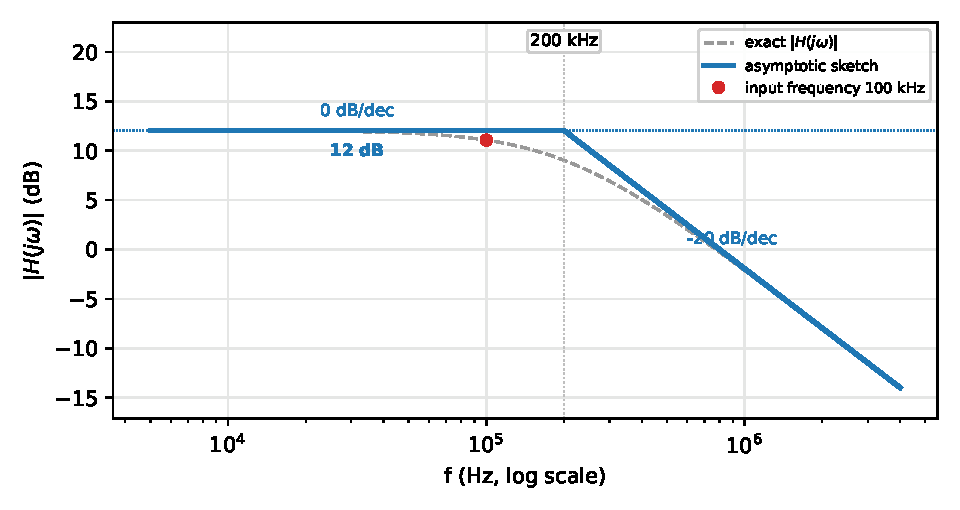
\includegraphics[width=0.78\linewidth,height=6.5cm,keepaspectratio]{p02_bode}\end{center}

{\small Blue: the straight-line sketch you are expected to draw. Dashed grey: the exact curve (about 3\,dB below the corner of an isolated pole). Red dot: the input frequency of Step 7.}
\solstep{7}{Steady-state output}The input is $V_i(t) = 0.2\sin\left(2\pi\cdot 10^{5}\,t\right)$, so $\omega_{in} = 2\pi\cdot 10^{5} = 6.28\times 10^{5}$\,rad/s. Put $s=j\omega_{in}$ in each factor (tool T5): magnitudes multiply, angles add.
{\small Rules: $\left|\frac{s}{s+p}\right| = \frac{\omega}{\sqrt{\omega^2+p^2}}$, $\angle = \frac{\pi}{2}-\tan^{-1}\frac{\omega}{p}$;\quad $\left|\frac{1}{1+s/p}\right| = \frac{1}{\sqrt{1+(\omega/p)^2}}$, $\angle = -\tan^{-1}\frac{\omega}{p}$;\quad $\left|1+\frac{s}{z}\right| = \sqrt{1+(\omega/z)^2}$, $\angle = \tan^{-1}\frac{\omega}{z}$;\quad a negative $K$ adds $-\pi$.}
\begin{center}\renewcommand{\arraystretch}{1.35}
\begin{tabular}{ccc}
\toprule
factor & magnitude & angle (rad) \\
\midrule
$-4$ & $4$ & $-3.14$ \\
$\rule[-1.7em]{0pt}{4em}\dfrac{1}{1+\dfrac{s}{2\pi\cdot 200\mathrm{k}}}$ & $0.8944$ & $-0.464$ \\
\textbf{total} & $\mathbf{3.578}$ (product) & $\mathbf{-3.61}$ (sum) \\
\bottomrule
\end{tabular}\end{center}

\begin{align*}
|H(j\omega_{in})| &= 3.58, \qquad \angle H(j\omega_{in}) = -3.61\ \mathrm{rad} \\
v_{o,ac}(t) &= 3.58\times 0.2\,\sin\left(2\pi\cdot 10^{5}\,t - 3.61\right) = 0.716\,\sin\left(2\pi\cdot 10^{5}\,t - 3.61\right)
\end{align*}

\[
\boxed{V_o(t) = 0.716\,\sin\left(2\pi\cdot 10^{5}\,t - 3.61\right)\ \mathrm{V}}
\]

\begin{ansbox}
$H(s) = -4\,\dfrac{1}{1+\dfrac{s}{2\pi\cdot 200\mathrm{k}}}$\quad (corners: 200 kHz)\\[4pt]
$V_o(t) = 0.716\,\sin\left(2\pi\cdot 10^{5}\,t - 3.61\right)\ \mathrm{V}$
\end{ansbox}

\newpage
\subsection*{Solution 2D.3 \hfill Easy}
\begin{center}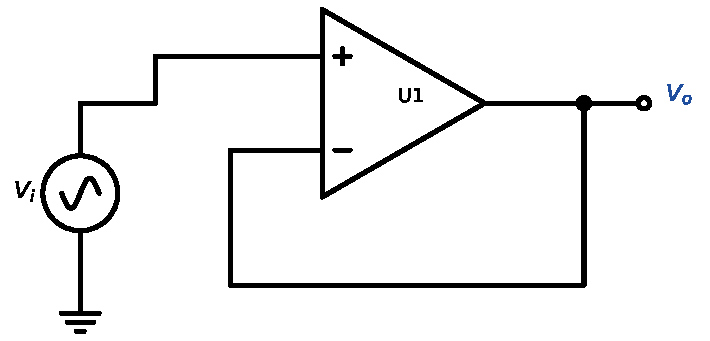
\includegraphics[width=\linewidth,height=5cm,keepaspectratio]{p03_circuit}\end{center}
\solstep{1}{Identify the sources}Independent sources: the AC input $V_i(t)$. No DC source: $V_{o,dc}=0$ and Step 2 is skipped.
\solstep{2}{DC circuit}No DC sources: $V_{o,dc}=0$.
\solstep{3}{Op-amp model}Non-ideal op-amp model (tool T5): $V_{out} = A(s)\,(V_+-V_-)$ with $A(s)=\dfrac{A_0}{1+s/\omega_b}$, $A_0=10^{5}$, $\omega_b = 2\pi\cdot20 = 126$\,rad/s, so the unity-gain frequency is $\omega_t = A_0\omega_b = 1.26\times 10^{7}$\,rad/s. The virtual short is \emph{not} used; only ``no current into the inputs'' is still true.

\solstep{4}{Transfer function, op-amp by op-amp}Recipe for each op-amp: write $V_+$ and $V_-$ by superposition of the block input and the op-amp output (each alone is a plain divider): $V_+ = \alpha_+V_{in}$, $V_- = \alpha_-V_{in}+\beta V_{out}$. Then $V_{out} = A(\alpha_+-\alpha_-)V_{in} - A\beta V_{out}$, i.e.\[
\frac{V_{out}}{V_{in}} = \frac{A(\alpha_+-\alpha_-)}{1+A\beta} = \frac{G}{1+\dfrac{1}{A\beta}},\qquad G = \frac{\alpha_+-\alpha_-}{\beta}\ \text{(the ideal gain)}
\]
With $A(s)$ inserted and constant $\alpha,\beta$:\[
\frac{V_{out}}{V_{in}} = G\,\frac{A_0\beta}{1+A_0\beta}\cdot\frac{1}{1+\dfrac{s}{\omega_b(1+A_0\beta)}},\qquad \omega_b(1+A_0\beta)\approx\beta\,\omega_t
\]

\textbf{Block 1 (U1).} (no current enters either input, so both are plain dividers)\begin{align*}
V_+ &= V_{i} \\
V_- &= V_{o}
\end{align*}
So $\alpha_+ = 1$, $\alpha_- = 0$, $\beta = 1$: ideal gain $G = \frac{\alpha_+-\alpha_-}{\beta} = 1$, $A_0\beta = 10^{5}$.\[
\frac{V_{o}}{V_{i}} = 1\cdot\frac{10^{5}}{1+10^{5}}\cdot\frac{1}{1+\dfrac{s}{1.26\times 10^{7}}} = \frac{1}{1+\dfrac{s}{1.26\times 10^{7}}}
\]
(closed-loop bandwidth $\omega_b(1+A_0\beta) = 1.26\times 10^{7}$\,rad/s, $f = 2 MHz$; compare $\beta\omega_t = 1.26\times 10^{7}$\,rad/s.)
So:\[
H(s) = \dfrac{1.26\times 10^{7}}{s + 1.26\times 10^{7}}
\]

\solstep{5}{Standard (Bode-ready) form}Find the roots. Every root $s=-p$ of the denominator is a \emph{pole}, every root $s=-z$ of the numerator is a \emph{zero}; $|p|$ and $|z|$ are the corner frequencies (rad/s).
\begin{itemize}[leftmargin=*,itemsep=2pt]
\item Denominator: $s + 1.26\times 10^{7}$; $s + 1.26\times 10^{7} = 0 \Rightarrow s = -1.26\times 10^{7}$.
\end{itemize}

Factored form (leading coefficient in front):
\[
H(s) = 1.26\times 10^{7}\,\dfrac{1}{(s+1.26\times 10^{7})}
\]

Bode-ready form: rewrite every $(s+p) = p\left(1+\frac{s}{p}\right)$ and $(s+z) = z\left(1+\frac{s}{z}\right)$, and collect all constants into $K$. Then every factor except $K$ is $\approx 1$ inside the pass-band:
\[
H(s) = 1\,\dfrac{1}{1+\dfrac{s}{2\pi\cdot 2\mathrm{M}}},\qquad K = 1
\]

\begin{center}\renewcommand{\arraystretch}{1.35}
\begin{tabular}{cccc}
\toprule
type & $\omega_c$ (rad/s) & $f_c=\omega_c/2\pi$ & slope change \\
\midrule
pole & $1.26\times 10^{7}$ & 2 MHz & $-20$ dB/dec \\
\bottomrule
\end{tabular}\end{center}

\solstep{6}{Magnitude Bode plot}Below every corner, all factors are $\approx$ constant: $|H| \approx 1$ $= -0.0000869$\,dB (flat, 0 dB/dec). Then, moving right, each pole bends the line down by 20\,dB/dec and each zero bends it up by 20\,dB/dec (tool T6):
\begin{center}\renewcommand{\arraystretch}{1.35}
\begin{tabular}{lcl}
\toprule
frequency range & slope & asymptote level \\
\midrule
$f<$ 2 MHz & $0$ dB/dec (flat) & -0.0000869 dB at end \\
$f>$ 2 MHz & $-20$ dB/dec & -0.0000869 dB at start \\
\bottomrule
\end{tabular}\end{center}

The flat (pass-band) level is $20\log_{10}|K| = 20\log_{10}1 = -0.0000869$\,dB.
\begin{center}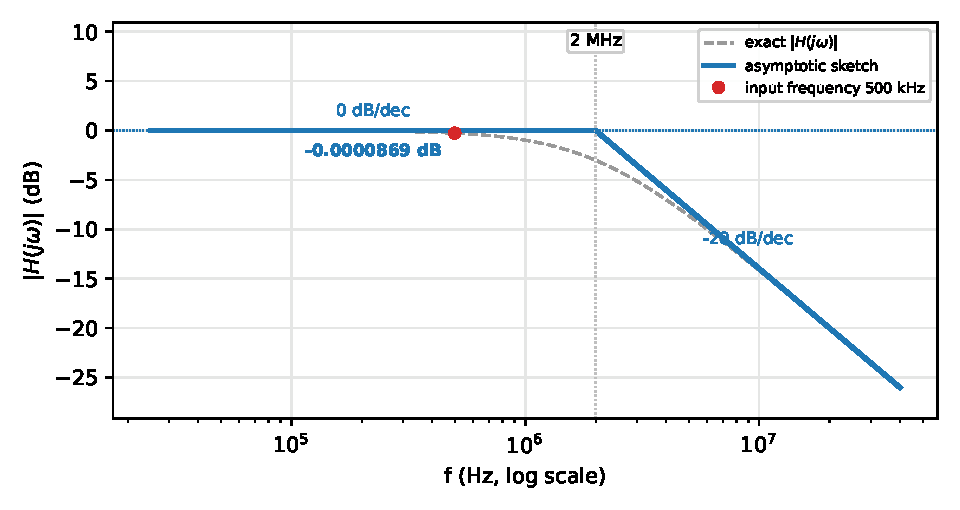
\includegraphics[width=0.78\linewidth,height=6.5cm,keepaspectratio]{p03_bode}\end{center}

{\small Blue: the straight-line sketch you are expected to draw. Dashed grey: the exact curve (about 3\,dB below the corner of an isolated pole). Red dot: the input frequency of Step 7.}
\solstep{7}{Steady-state output}The input is $V_i(t) = 1\sin\left(2\pi\cdot 5\times 10^{5}\,t\right)$, so $\omega_{in} = 2\pi\cdot 5\times 10^{5} = 3.14\times 10^{6}$\,rad/s. Put $s=j\omega_{in}$ in each factor (tool T5): magnitudes multiply, angles add.
{\small Rules: $\left|\frac{s}{s+p}\right| = \frac{\omega}{\sqrt{\omega^2+p^2}}$, $\angle = \frac{\pi}{2}-\tan^{-1}\frac{\omega}{p}$;\quad $\left|\frac{1}{1+s/p}\right| = \frac{1}{\sqrt{1+(\omega/p)^2}}$, $\angle = -\tan^{-1}\frac{\omega}{p}$;\quad $\left|1+\frac{s}{z}\right| = \sqrt{1+(\omega/z)^2}$, $\angle = \tan^{-1}\frac{\omega}{z}$;\quad a negative $K$ adds $-\pi$.}
\begin{center}\renewcommand{\arraystretch}{1.35}
\begin{tabular}{ccc}
\toprule
factor & magnitude & angle (rad) \\
\midrule
$1$ & $1$ & $0$ \\
$\rule[-1.7em]{0pt}{4em}\dfrac{1}{1+\dfrac{s}{2\pi\cdot 2\mathrm{M}}}$ & $0.9701$ & $-0.245$ \\
\textbf{total} & $\mathbf{0.9701}$ (product) & $\mathbf{-0.245}$ (sum) \\
\bottomrule
\end{tabular}\end{center}

\begin{align*}
|H(j\omega_{in})| &= 0.97, \qquad \angle H(j\omega_{in}) = -0.245\ \mathrm{rad} \\
v_{o,ac}(t) &= 0.97\times 1\,\sin\left(2\pi\cdot 5\times 10^{5}\,t - 0.245\right) = 0.97\,\sin\left(2\pi\cdot 5\times 10^{5}\,t - 0.245\right)
\end{align*}

\[
\boxed{V_o(t) = 0.97\,\sin\left(2\pi\cdot 5\times 10^{5}\,t - 0.245\right)\ \mathrm{V}}
\]

\begin{ansbox}
$H(s) = 1\,\dfrac{1}{1+\dfrac{s}{2\pi\cdot 2\mathrm{M}}}$\quad (corners: 2 MHz)\\[4pt]
$V_o(t) = 0.97\,\sin\left(2\pi\cdot 5\times 10^{5}\,t - 0.245\right)\ \mathrm{V}$
\end{ansbox}

\newpage
\subsection*{Solution 2D.4 \hfill Easy}
\begin{center}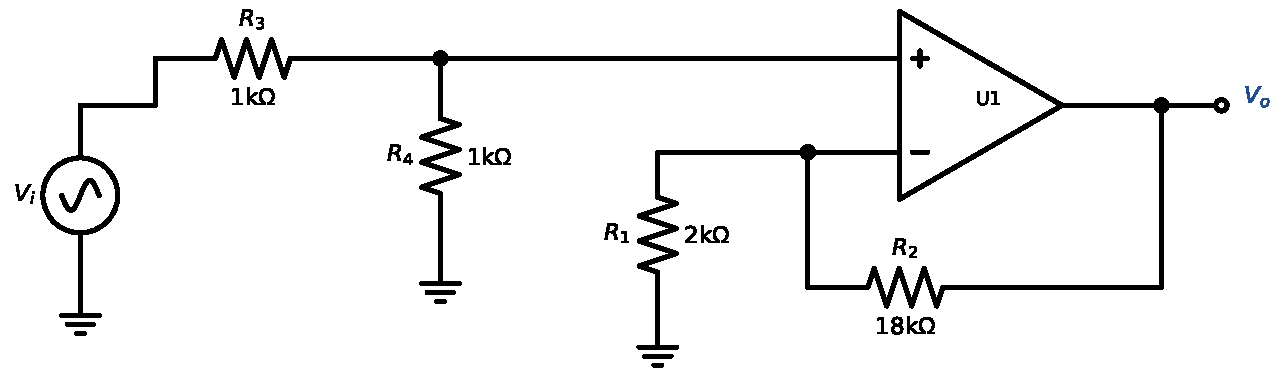
\includegraphics[width=\linewidth,height=5cm,keepaspectratio]{p04_circuit}\end{center}
\solstep{1}{Identify the sources}Independent sources: the AC input $V_i(t)$. No DC source: $V_{o,dc}=0$ and Step 2 is skipped.
\solstep{2}{DC circuit}No DC sources: $V_{o,dc}=0$.
\solstep{3}{Op-amp model}Non-ideal op-amp model (tool T5): $V_{out} = A(s)\,(V_+-V_-)$ with $A(s)=\dfrac{A_0}{1+s/\omega_b}$, $A_0=10^{5}$, $\omega_b = 2\pi\cdot10 = 62.8$\,rad/s, so the unity-gain frequency is $\omega_t = A_0\omega_b = 6.28\times 10^{6}$\,rad/s. The virtual short is \emph{not} used; only ``no current into the inputs'' is still true.

\solstep{4}{Transfer function, op-amp by op-amp}Recipe for each op-amp: write $V_+$ and $V_-$ by superposition of the block input and the op-amp output (each alone is a plain divider): $V_+ = \alpha_+V_{in}$, $V_- = \alpha_-V_{in}+\beta V_{out}$. Then $V_{out} = A(\alpha_+-\alpha_-)V_{in} - A\beta V_{out}$, i.e.\[
\frac{V_{out}}{V_{in}} = \frac{A(\alpha_+-\alpha_-)}{1+A\beta} = \frac{G}{1+\dfrac{1}{A\beta}},\qquad G = \frac{\alpha_+-\alpha_-}{\beta}\ \text{(the ideal gain)}
\]
With $A(s)$ inserted and constant $\alpha,\beta$:\[
\frac{V_{out}}{V_{in}} = G\,\frac{A_0\beta}{1+A_0\beta}\cdot\frac{1}{1+\dfrac{s}{\omega_b(1+A_0\beta)}},\qquad \omega_b(1+A_0\beta)\approx\beta\,\omega_t
\]

\textbf{Block 1 (U1).} (no current enters either input, so both are plain dividers)\begin{align*}
V_+ &= \frac{R_{4}}{R_{3} + R_{4}}V_{i} \\
V_- &= \frac{R_{1}}{R_{1}+R_{2}}V_{o}
\end{align*}
So $\alpha_+ = 0.5$, $\alpha_- = 0$, $\beta = 0.1$: ideal gain $G = \frac{\alpha_+-\alpha_-}{\beta} = 5$, $A_0\beta = 10000$.\[
\frac{V_{o}}{V_{i}} = 5\cdot\frac{10000}{1+10000}\cdot\frac{1}{1+\dfrac{s}{6.28\times 10^{5}}} = \frac{5}{1+\dfrac{s}{6.28\times 10^{5}}}
\]
(closed-loop bandwidth $\omega_b(1+A_0\beta) = 6.28\times 10^{5}$\,rad/s, $f = 100 kHz$; compare $\beta\omega_t = 6.28\times 10^{5}$\,rad/s.)
So:\[
H(s) = \dfrac{3.14\times 10^{6}}{s + 6.28\times 10^{5}}
\]

\solstep{5}{Standard (Bode-ready) form}Find the roots. Every root $s=-p$ of the denominator is a \emph{pole}, every root $s=-z$ of the numerator is a \emph{zero}; $|p|$ and $|z|$ are the corner frequencies (rad/s).
\begin{itemize}[leftmargin=*,itemsep=2pt]
\item Denominator: $s + 6.28\times 10^{5}$; $s + 6.28\times 10^{5} = 0 \Rightarrow s = -6.28\times 10^{5}$.
\end{itemize}

Factored form (leading coefficient in front):
\[
H(s) = 3.14\times 10^{6}\,\dfrac{1}{(s+6.28\times 10^{5})}
\]

Bode-ready form: rewrite every $(s+p) = p\left(1+\frac{s}{p}\right)$ and $(s+z) = z\left(1+\frac{s}{z}\right)$, and collect all constants into $K$. Then every factor except $K$ is $\approx 1$ inside the pass-band:
\[
H(s) = 5\,\dfrac{1}{1+\dfrac{s}{2\pi\cdot 100\mathrm{k}}},\qquad K = 5
\]

\begin{center}\renewcommand{\arraystretch}{1.35}
\begin{tabular}{cccc}
\toprule
type & $\omega_c$ (rad/s) & $f_c=\omega_c/2\pi$ & slope change \\
\midrule
pole & $6.28\times 10^{5}$ & 100 kHz & $-20$ dB/dec \\
\bottomrule
\end{tabular}\end{center}

\solstep{6}{Magnitude Bode plot}Below every corner, all factors are $\approx$ constant: $|H| \approx 5$ $= 14$\,dB (flat, 0 dB/dec). Then, moving right, each pole bends the line down by 20\,dB/dec and each zero bends it up by 20\,dB/dec (tool T6):
\begin{center}\renewcommand{\arraystretch}{1.35}
\begin{tabular}{lcl}
\toprule
frequency range & slope & asymptote level \\
\midrule
$f<$ 100 kHz & $0$ dB/dec (flat) & 14 dB at end \\
$f>$ 100 kHz & $-20$ dB/dec & 14 dB at start \\
\bottomrule
\end{tabular}\end{center}

The flat (pass-band) level is $20\log_{10}|K| = 20\log_{10}5 = 14$\,dB.
\begin{center}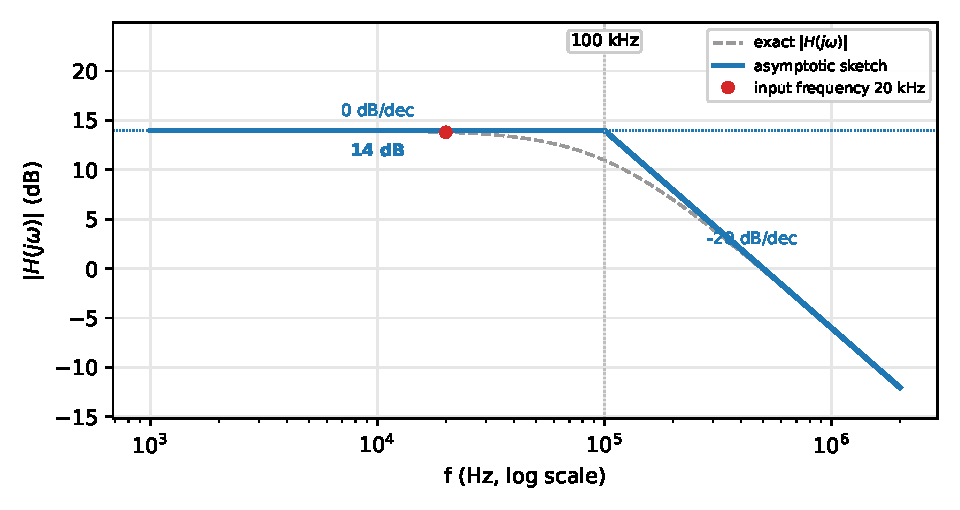
\includegraphics[width=0.78\linewidth,height=6.5cm,keepaspectratio]{p04_bode}\end{center}

{\small Blue: the straight-line sketch you are expected to draw. Dashed grey: the exact curve (about 3\,dB below the corner of an isolated pole). Red dot: the input frequency of Step 7.}
\solstep{7}{Steady-state output}The input is $V_i(t) = 0.2\sin\left(2\pi\cdot 20000\,t\right)$, so $\omega_{in} = 2\pi\cdot 20000 = 1.26\times 10^{5}$\,rad/s. Put $s=j\omega_{in}$ in each factor (tool T5): magnitudes multiply, angles add.
{\small Rules: $\left|\frac{s}{s+p}\right| = \frac{\omega}{\sqrt{\omega^2+p^2}}$, $\angle = \frac{\pi}{2}-\tan^{-1}\frac{\omega}{p}$;\quad $\left|\frac{1}{1+s/p}\right| = \frac{1}{\sqrt{1+(\omega/p)^2}}$, $\angle = -\tan^{-1}\frac{\omega}{p}$;\quad $\left|1+\frac{s}{z}\right| = \sqrt{1+(\omega/z)^2}$, $\angle = \tan^{-1}\frac{\omega}{z}$;\quad a negative $K$ adds $-\pi$.}
\begin{center}\renewcommand{\arraystretch}{1.35}
\begin{tabular}{ccc}
\toprule
factor & magnitude & angle (rad) \\
\midrule
$5$ & $5$ & $0$ \\
$\rule[-1.7em]{0pt}{4em}\dfrac{1}{1+\dfrac{s}{2\pi\cdot 100\mathrm{k}}}$ & $0.9806$ & $-0.197$ \\
\textbf{total} & $\mathbf{4.902}$ (product) & $\mathbf{-0.197}$ (sum) \\
\bottomrule
\end{tabular}\end{center}

\begin{align*}
|H(j\omega_{in})| &= 4.9, \qquad \angle H(j\omega_{in}) = -0.197\ \mathrm{rad} \\
v_{o,ac}(t) &= 4.9\times 0.2\,\sin\left(2\pi\cdot 20000\,t - 0.197\right) = 0.98\,\sin\left(2\pi\cdot 20000\,t - 0.197\right)
\end{align*}

\[
\boxed{V_o(t) = 0.98\,\sin\left(2\pi\cdot 20000\,t - 0.197\right)\ \mathrm{V}}
\]

\begin{ansbox}
$H(s) = 5\,\dfrac{1}{1+\dfrac{s}{2\pi\cdot 100\mathrm{k}}}$\quad (corners: 100 kHz)\\[4pt]
$V_o(t) = 0.98\,\sin\left(2\pi\cdot 20000\,t - 0.197\right)\ \mathrm{V}$
\end{ansbox}

\newpage
\subsection*{Solution 2D.5 \hfill Easy}
\begin{center}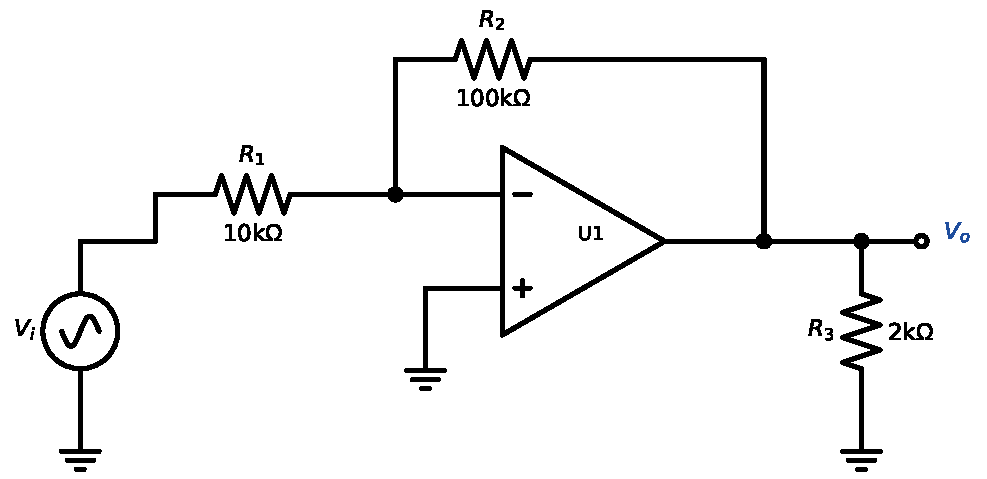
\includegraphics[width=\linewidth,height=5cm,keepaspectratio]{p05_circuit}\end{center}
\solstep{1}{Identify the sources}Independent sources: the AC input $V_i(t)$. No DC source: $V_{o,dc}=0$ and Step 2 is skipped.
\solstep{2}{DC circuit}No DC sources: $V_{o,dc}=0$.
\solstep{3}{Op-amp model}Non-ideal op-amp model (tool T5): $V_{out} = A(s)\,(V_+-V_-)$ with $A(s)=\dfrac{A_0}{1+s/\omega_b}$, $A_0=10^{5}$, $\omega_b = 2\pi\cdot10 = 62.8$\,rad/s, so the unity-gain frequency is $\omega_t = A_0\omega_b = 6.28\times 10^{6}$\,rad/s. The virtual short is \emph{not} used; only ``no current into the inputs'' is still true.

\solstep{4}{Transfer function, op-amp by op-amp}Recipe for each op-amp: write $V_+$ and $V_-$ by superposition of the block input and the op-amp output (each alone is a plain divider): $V_+ = \alpha_+V_{in}$, $V_- = \alpha_-V_{in}+\beta V_{out}$. Then $V_{out} = A(\alpha_+-\alpha_-)V_{in} - A\beta V_{out}$, i.e.\[
\frac{V_{out}}{V_{in}} = \frac{A(\alpha_+-\alpha_-)}{1+A\beta} = \frac{G}{1+\dfrac{1}{A\beta}},\qquad G = \frac{\alpha_+-\alpha_-}{\beta}\ \text{(the ideal gain)}
\]
With $A(s)$ inserted and constant $\alpha,\beta$:\[
\frac{V_{out}}{V_{in}} = G\,\frac{A_0\beta}{1+A_0\beta}\cdot\frac{1}{1+\dfrac{s}{\omega_b(1+A_0\beta)}},\qquad \omega_b(1+A_0\beta)\approx\beta\,\omega_t
\]

The load $R_{3}$ sits on an op-amp output, modelled as the ideal source $A(V_+-V_-)$: it does not change the output voltage and drops out.
\textbf{Block 1 (U1).} (superposition: $V_{i}$ alone with $V_{o}=0$ gives a divider $R_{1}$--$R_{2}$, and vice versa)\begin{align*}
V_+ &= 0 \quad(\text{grounded}) \\
V_- &= \frac{R_{2}}{R_{1}+R_{2}}V_{i} + \frac{R_{1}}{R_{1}+R_{2}}V_{o}
\end{align*}
So $\alpha_+ = 0$, $\alpha_- = 0.9091$, $\beta = 0.09091$: ideal gain $G = \frac{\alpha_+-\alpha_-}{\beta} = -10$, $A_0\beta = 9090$.\[
\frac{V_{o}}{V_{i}} = -10\cdot\frac{9090}{1+9090}\cdot\frac{1}{1+\dfrac{s}{5.71\times 10^{5}}} = \frac{-9.999}{1+\dfrac{s}{5.71\times 10^{5}}}
\]
(closed-loop bandwidth $\omega_b(1+A_0\beta) = 5.71\times 10^{5}$\,rad/s, $f = 90.9 kHz$; compare $\beta\omega_t = 5.71\times 10^{5}$\,rad/s.)
So:\[
H(s) = \dfrac{-5.71\times 10^{6}}{s + 5.71\times 10^{5}}
\]

\solstep{5}{Standard (Bode-ready) form}Find the roots. Every root $s=-p$ of the denominator is a \emph{pole}, every root $s=-z$ of the numerator is a \emph{zero}; $|p|$ and $|z|$ are the corner frequencies (rad/s).
\begin{itemize}[leftmargin=*,itemsep=2pt]
\item Denominator: $s + 5.71\times 10^{5}$; $s + 5.71\times 10^{5} = 0 \Rightarrow s = -5.71\times 10^{5}$.
\end{itemize}

Factored form (leading coefficient in front):
\[
H(s) = -5.71\times 10^{6}\,\dfrac{1}{(s+5.71\times 10^{5})}
\]

Bode-ready form: rewrite every $(s+p) = p\left(1+\frac{s}{p}\right)$ and $(s+z) = z\left(1+\frac{s}{z}\right)$, and collect all constants into $K$. Then every factor except $K$ is $\approx 1$ inside the pass-band:
\[
H(s) = -10\,\dfrac{1}{1+\dfrac{s}{2\pi\cdot 90.9\mathrm{k}}},\qquad K = -10
\]

\begin{center}\renewcommand{\arraystretch}{1.35}
\begin{tabular}{cccc}
\toprule
type & $\omega_c$ (rad/s) & $f_c=\omega_c/2\pi$ & slope change \\
\midrule
pole & $5.71\times 10^{5}$ & 90.9 kHz & $-20$ dB/dec \\
\bottomrule
\end{tabular}\end{center}

\solstep{6}{Magnitude Bode plot}Below every corner, all factors are $\approx$ constant: $|H| \approx 10$ $= 20$\,dB (flat, 0 dB/dec). Then, moving right, each pole bends the line down by 20\,dB/dec and each zero bends it up by 20\,dB/dec (tool T6):
\begin{center}\renewcommand{\arraystretch}{1.35}
\begin{tabular}{lcl}
\toprule
frequency range & slope & asymptote level \\
\midrule
$f<$ 90.9 kHz & $0$ dB/dec (flat) & 20 dB at end \\
$f>$ 90.9 kHz & $-20$ dB/dec & 20 dB at start \\
\bottomrule
\end{tabular}\end{center}

The flat (pass-band) level is $20\log_{10}|K| = 20\log_{10}10 = 20$\,dB.
\begin{center}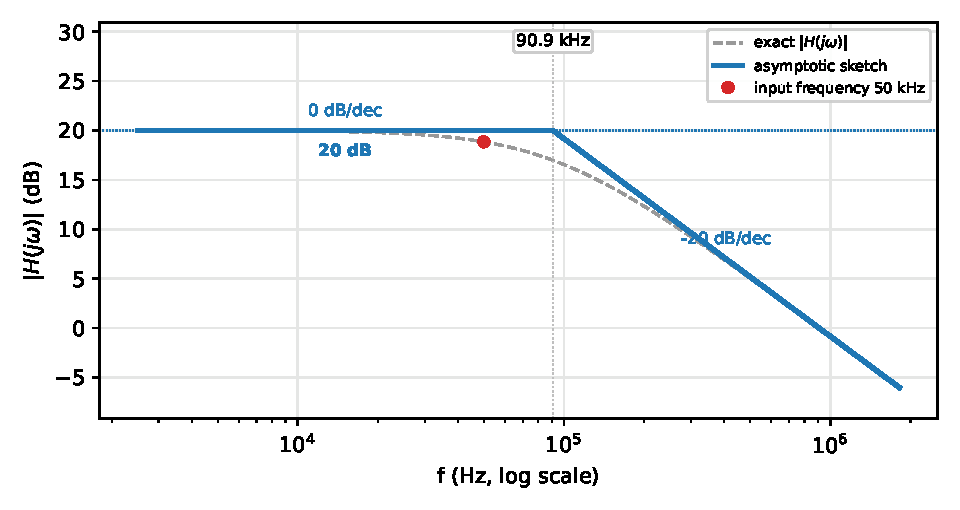
\includegraphics[width=0.78\linewidth,height=6.5cm,keepaspectratio]{p05_bode}\end{center}

{\small Blue: the straight-line sketch you are expected to draw. Dashed grey: the exact curve (about 3\,dB below the corner of an isolated pole). Red dot: the input frequency of Step 7.}
\solstep{7}{Steady-state output}The input is $V_i(t) = 0.05\sin\left(2\pi\cdot 50000\,t\right)$, so $\omega_{in} = 2\pi\cdot 50000 = 3.14\times 10^{5}$\,rad/s. Put $s=j\omega_{in}$ in each factor (tool T5): magnitudes multiply, angles add.
{\small Rules: $\left|\frac{s}{s+p}\right| = \frac{\omega}{\sqrt{\omega^2+p^2}}$, $\angle = \frac{\pi}{2}-\tan^{-1}\frac{\omega}{p}$;\quad $\left|\frac{1}{1+s/p}\right| = \frac{1}{\sqrt{1+(\omega/p)^2}}$, $\angle = -\tan^{-1}\frac{\omega}{p}$;\quad $\left|1+\frac{s}{z}\right| = \sqrt{1+(\omega/z)^2}$, $\angle = \tan^{-1}\frac{\omega}{z}$;\quad a negative $K$ adds $-\pi$.}
\begin{center}\renewcommand{\arraystretch}{1.35}
\begin{tabular}{ccc}
\toprule
factor & magnitude & angle (rad) \\
\midrule
$-10$ & $9.999$ & $-3.14$ \\
$\rule[-1.7em]{0pt}{4em}\dfrac{1}{1+\dfrac{s}{2\pi\cdot 90.9\mathrm{k}}}$ & $0.8762$ & $-0.503$ \\
\textbf{total} & $\mathbf{8.761}$ (product) & $\mathbf{-3.64}$ (sum) \\
\bottomrule
\end{tabular}\end{center}

\begin{align*}
|H(j\omega_{in})| &= 8.76, \qquad \angle H(j\omega_{in}) = -3.64\ \mathrm{rad} \\
v_{o,ac}(t) &= 8.76\times 0.05\,\sin\left(2\pi\cdot 50000\,t - 3.64\right) = 0.438\,\sin\left(2\pi\cdot 50000\,t - 3.64\right)
\end{align*}

\[
\boxed{V_o(t) = 0.438\,\sin\left(2\pi\cdot 50000\,t - 3.64\right)\ \mathrm{V}}
\]

\begin{ansbox}
$H(s) = -10\,\dfrac{1}{1+\dfrac{s}{2\pi\cdot 90.9\mathrm{k}}}$\quad (corners: 90.9 kHz)\\[4pt]
$V_o(t) = 0.438\,\sin\left(2\pi\cdot 50000\,t - 3.64\right)\ \mathrm{V}$
\end{ansbox}

\newpage
\subsection*{Solution 2D.6 \hfill Easy}
\begin{center}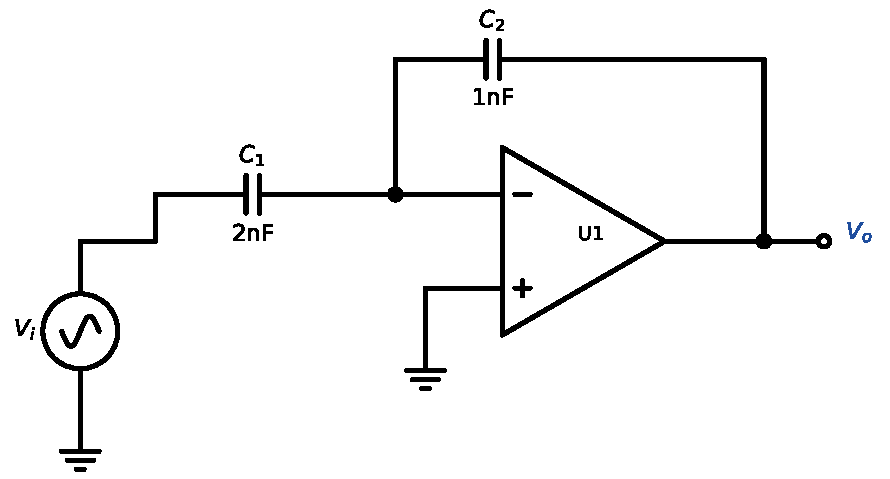
\includegraphics[width=\linewidth,height=5cm,keepaspectratio]{p06_circuit}\end{center}
\solstep{1}{Identify the sources}Independent sources: the AC input $V_i(t)$. No DC source: $V_{o,dc}=0$ and Step 2 is skipped.
\solstep{2}{DC circuit}No DC sources: $V_{o,dc}=0$.
\solstep{3}{Op-amp model}Non-ideal op-amp model (tool T5): $V_{out} = A(s)\,(V_+-V_-)$ with $A(s)=\dfrac{A_0}{1+s/\omega_b}$, $A_0=10^{5}$, $\omega_b = 2\pi\cdot10 = 62.8$\,rad/s, so the unity-gain frequency is $\omega_t = A_0\omega_b = 6.28\times 10^{6}$\,rad/s. The virtual short is \emph{not} used; only ``no current into the inputs'' is still true.

\solstep{4}{Transfer function, op-amp by op-amp}Recipe for each op-amp: write $V_+$ and $V_-$ by superposition of the block input and the op-amp output (each alone is a plain divider): $V_+ = \alpha_+V_{in}$, $V_- = \alpha_-V_{in}+\beta V_{out}$. Then $V_{out} = A(\alpha_+-\alpha_-)V_{in} - A\beta V_{out}$, i.e.\[
\frac{V_{out}}{V_{in}} = \frac{A(\alpha_+-\alpha_-)}{1+A\beta} = \frac{G}{1+\dfrac{1}{A\beta}},\qquad G = \frac{\alpha_+-\alpha_-}{\beta}\ \text{(the ideal gain)}
\]
With $A(s)$ inserted and constant $\alpha,\beta$:\[
\frac{V_{out}}{V_{in}} = G\,\frac{A_0\beta}{1+A_0\beta}\cdot\frac{1}{1+\dfrac{s}{\omega_b(1+A_0\beta)}},\qquad \omega_b(1+A_0\beta)\approx\beta\,\omega_t
\]

\textbf{Block 1 (U1).} (superposition: $V_{i}$ alone with $V_{o}=0$ gives a divider $\frac{1}{sC_{1}}$--$\frac{1}{sC_{2}}$, and vice versa)\begin{align*}
V_+ &= 0 \quad(\text{grounded}) \\
V_- &= \frac{\frac{1}{sC_{2}}}{\frac{1}{sC_{1}}+\frac{1}{sC_{2}}}V_{i} + \frac{\frac{1}{sC_{1}}}{\frac{1}{sC_{1}}+\frac{1}{sC_{2}}}V_{o}
\end{align*}
(Only capacitors: every impedance is $\frac{1}{sC}$, so in each ratio the $s$ cancels, e.g. $\frac{1/(sC_a)}{1/(sC_a)+1/(sC_b)} = \frac{C_b}{C_a+C_b}$, and $\frac{1}{sC_a}\parallel\frac{1}{sC_b} = \frac{1}{s(C_a+C_b)}$.) So $\alpha_+ = 0$, $\alpha_- = 0.6667$, $\beta = 0.3333$: ideal gain $G = \frac{\alpha_+-\alpha_-}{\beta} = -2$, $A_0\beta = 33300$.\[
\frac{V_{o}}{V_{i}} = -2\cdot\frac{33300}{1+33300}\cdot\frac{1}{1+\dfrac{s}{2.09\times 10^{6}}} = \frac{-2}{1+\dfrac{s}{2.09\times 10^{6}}}
\]
(closed-loop bandwidth $\omega_b(1+A_0\beta) = 2.09\times 10^{6}$\,rad/s, $f = 333 kHz$; compare $\beta\omega_t = 2.09\times 10^{6}$\,rad/s.)
So:\[
H(s) = \dfrac{-4.19\times 10^{6}}{s + 2.09\times 10^{6}}
\]

\solstep{5}{Standard (Bode-ready) form}Find the roots. Every root $s=-p$ of the denominator is a \emph{pole}, every root $s=-z$ of the numerator is a \emph{zero}; $|p|$ and $|z|$ are the corner frequencies (rad/s).
\begin{itemize}[leftmargin=*,itemsep=2pt]
\item Denominator: $s + 2.09\times 10^{6}$; $s + 2.09\times 10^{6} = 0 \Rightarrow s = -2.09\times 10^{6}$.
\end{itemize}

Factored form (leading coefficient in front):
\[
H(s) = -4.19\times 10^{6}\,\dfrac{1}{(s+2.09\times 10^{6})}
\]

Bode-ready form: rewrite every $(s+p) = p\left(1+\frac{s}{p}\right)$ and $(s+z) = z\left(1+\frac{s}{z}\right)$, and collect all constants into $K$. Then every factor except $K$ is $\approx 1$ inside the pass-band:
\[
H(s) = -2\,\dfrac{1}{1+\dfrac{s}{2\pi\cdot 333\mathrm{k}}},\qquad K = -2
\]

\begin{center}\renewcommand{\arraystretch}{1.35}
\begin{tabular}{cccc}
\toprule
type & $\omega_c$ (rad/s) & $f_c=\omega_c/2\pi$ & slope change \\
\midrule
pole & $2.09\times 10^{6}$ & 333 kHz & $-20$ dB/dec \\
\bottomrule
\end{tabular}\end{center}

\solstep{6}{Magnitude Bode plot}Below every corner, all factors are $\approx$ constant: $|H| \approx 2$ $= 6.02$\,dB (flat, 0 dB/dec). Then, moving right, each pole bends the line down by 20\,dB/dec and each zero bends it up by 20\,dB/dec (tool T6):
\begin{center}\renewcommand{\arraystretch}{1.35}
\begin{tabular}{lcl}
\toprule
frequency range & slope & asymptote level \\
\midrule
$f<$ 333 kHz & $0$ dB/dec (flat) & 6.02 dB at end \\
$f>$ 333 kHz & $-20$ dB/dec & 6.02 dB at start \\
\bottomrule
\end{tabular}\end{center}

The flat (pass-band) level is $20\log_{10}|K| = 20\log_{10}2 = 6.02$\,dB.
\begin{center}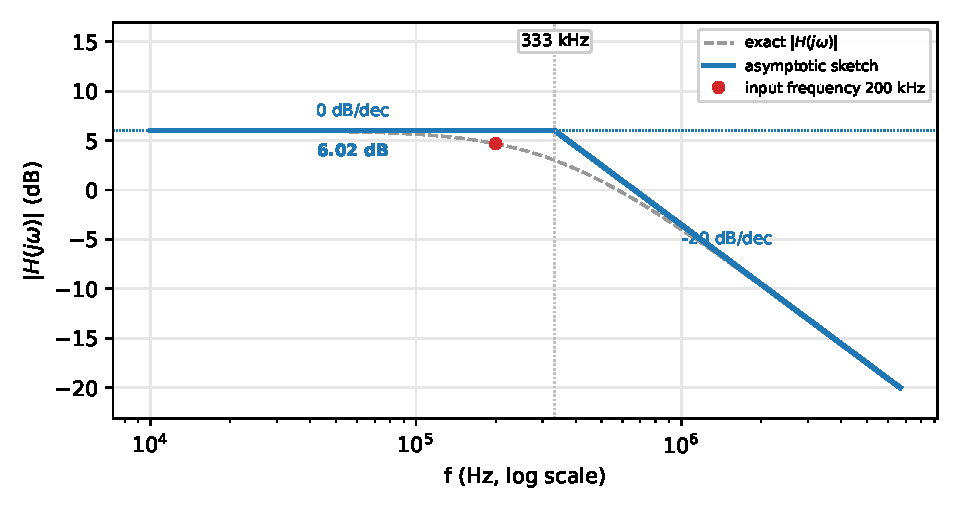
\includegraphics[width=0.78\linewidth,height=6.5cm,keepaspectratio]{p06_bode}\end{center}

{\small Blue: the straight-line sketch you are expected to draw. Dashed grey: the exact curve (about 3\,dB below the corner of an isolated pole). Red dot: the input frequency of Step 7.}
\solstep{7}{Steady-state output}The input is $V_i(t) = 0.2\sin\left(2\pi\cdot 2\times 10^{5}\,t\right)$, so $\omega_{in} = 2\pi\cdot 2\times 10^{5} = 1.26\times 10^{6}$\,rad/s. Put $s=j\omega_{in}$ in each factor (tool T5): magnitudes multiply, angles add.
{\small Rules: $\left|\frac{s}{s+p}\right| = \frac{\omega}{\sqrt{\omega^2+p^2}}$, $\angle = \frac{\pi}{2}-\tan^{-1}\frac{\omega}{p}$;\quad $\left|\frac{1}{1+s/p}\right| = \frac{1}{\sqrt{1+(\omega/p)^2}}$, $\angle = -\tan^{-1}\frac{\omega}{p}$;\quad $\left|1+\frac{s}{z}\right| = \sqrt{1+(\omega/z)^2}$, $\angle = \tan^{-1}\frac{\omega}{z}$;\quad a negative $K$ adds $-\pi$.}
\begin{center}\renewcommand{\arraystretch}{1.35}
\begin{tabular}{ccc}
\toprule
factor & magnitude & angle (rad) \\
\midrule
$-2$ & $2$ & $-3.14$ \\
$\rule[-1.7em]{0pt}{4em}\dfrac{1}{1+\dfrac{s}{2\pi\cdot 333\mathrm{k}}}$ & $0.8575$ & $-0.54$ \\
\textbf{total} & $\mathbf{1.715}$ (product) & $\mathbf{-3.68}$ (sum) \\
\bottomrule
\end{tabular}\end{center}

\begin{align*}
|H(j\omega_{in})| &= 1.71, \qquad \angle H(j\omega_{in}) = -3.68\ \mathrm{rad} \\
v_{o,ac}(t) &= 1.71\times 0.2\,\sin\left(2\pi\cdot 2\times 10^{5}\,t - 3.68\right) = 0.343\,\sin\left(2\pi\cdot 2\times 10^{5}\,t - 3.68\right)
\end{align*}

\[
\boxed{V_o(t) = 0.343\,\sin\left(2\pi\cdot 2\times 10^{5}\,t - 3.68\right)\ \mathrm{V}}
\]

\begin{ansbox}
$H(s) = -2\,\dfrac{1}{1+\dfrac{s}{2\pi\cdot 333\mathrm{k}}}$\quad (corners: 333 kHz)\\[4pt]
$V_o(t) = 0.343\,\sin\left(2\pi\cdot 2\times 10^{5}\,t - 3.68\right)\ \mathrm{V}$
\end{ansbox}

\newpage
\subsection*{Solution 2D.7 \hfill Medium}
\begin{center}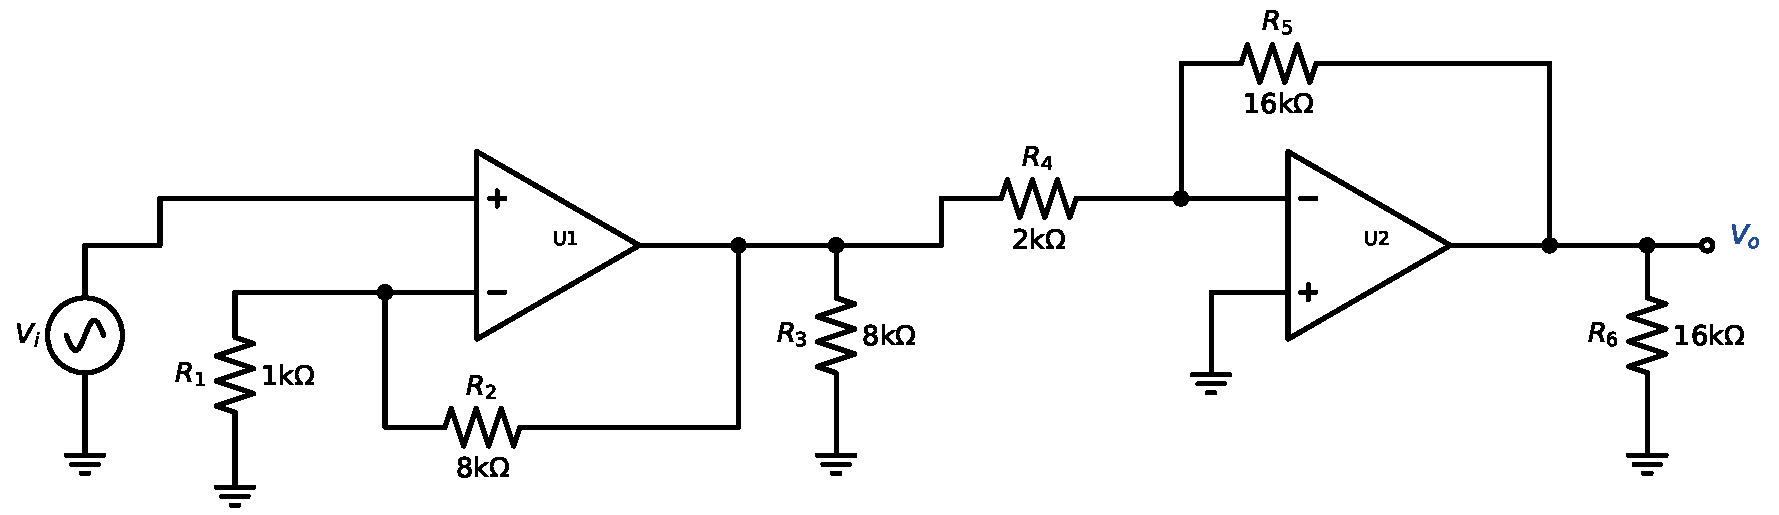
\includegraphics[width=\linewidth,height=5cm,keepaspectratio]{p07_circuit}\end{center}
\solstep{1}{Identify the sources}Independent sources: the AC input $V_i(t)$. No DC source: $V_{o,dc}=0$ and Step 2 is skipped.
\solstep{2}{DC circuit}No DC sources: $V_{o,dc}=0$.
\solstep{3}{Op-amp model}Non-ideal op-amp model (tool T5): $V_{out} = A(s)\,(V_+-V_-)$ with $A(s)=\dfrac{A_0}{1+s/\omega_b}$, $A_0=10^{5}$, $\omega_b = 2\pi\cdot20 = 126$\,rad/s, so the unity-gain frequency is $\omega_t = A_0\omega_b = 1.26\times 10^{7}$\,rad/s. The virtual short is \emph{not} used; only ``no current into the inputs'' is still true.

\solstep{4}{Transfer function, op-amp by op-amp}Recipe for each op-amp: write $V_+$ and $V_-$ by superposition of the block input and the op-amp output (each alone is a plain divider): $V_+ = \alpha_+V_{in}$, $V_- = \alpha_-V_{in}+\beta V_{out}$. Then $V_{out} = A(\alpha_+-\alpha_-)V_{in} - A\beta V_{out}$, i.e.\[
\frac{V_{out}}{V_{in}} = \frac{A(\alpha_+-\alpha_-)}{1+A\beta} = \frac{G}{1+\dfrac{1}{A\beta}},\qquad G = \frac{\alpha_+-\alpha_-}{\beta}\ \text{(the ideal gain)}
\]
With $A(s)$ inserted and constant $\alpha,\beta$:\[
\frac{V_{out}}{V_{in}} = G\,\frac{A_0\beta}{1+A_0\beta}\cdot\frac{1}{1+\dfrac{s}{\omega_b(1+A_0\beta)}},\qquad \omega_b(1+A_0\beta)\approx\beta\,\omega_t
\]

The load $R_{3}$, $R_{6}$ sits on an op-amp output, modelled as the ideal source $A(V_+-V_-)$: it does not change the output voltage and drops out.
\textbf{Block 1 (U1).} (no current enters either input, so both are plain dividers)\begin{align*}
V_+ &= V_{i} \\
V_- &= \frac{R_{1}}{R_{1}+R_{2}}V_{o1}
\end{align*}
So $\alpha_+ = 1$, $\alpha_- = 0$, $\beta = 0.1111$: ideal gain $G = \frac{\alpha_+-\alpha_-}{\beta} = 9$, $A_0\beta = 11100$.\[
\frac{V_{o1}}{V_{i}} = 9\cdot\frac{11100}{1+11100}\cdot\frac{1}{1+\dfrac{s}{1.4\times 10^{6}}} = \frac{8.999}{1+\dfrac{s}{1.4\times 10^{6}}}
\]
(closed-loop bandwidth $\omega_b(1+A_0\beta) = 1.4\times 10^{6}$\,rad/s, $f = 222 kHz$; compare $\beta\omega_t = 1.4\times 10^{6}$\,rad/s.)
\textbf{Block 2 (U2).} (superposition: $V_{o1}$ alone with $V_{o}=0$ gives a divider $R_{4}$--$R_{5}$, and vice versa)\begin{align*}
V_+ &= 0 \quad(\text{grounded}) \\
V_- &= \frac{R_{5}}{R_{4}+R_{5}}V_{o1} + \frac{R_{4}}{R_{4}+R_{5}}V_{o}
\end{align*}
So $\alpha_+ = 0$, $\alpha_- = 0.8889$, $\beta = 0.1111$: ideal gain $G = \frac{\alpha_+-\alpha_-}{\beta} = -8$, $A_0\beta = 11100$.\[
\frac{V_{o}}{V_{o1}} = -8\cdot\frac{11100}{1+11100}\cdot\frac{1}{1+\dfrac{s}{1.4\times 10^{6}}} = \frac{-7.999}{1+\dfrac{s}{1.4\times 10^{6}}}
\]
(closed-loop bandwidth $\omega_b(1+A_0\beta) = 1.4\times 10^{6}$\,rad/s, $f = 222 kHz$; compare $\beta\omega_t = 1.4\times 10^{6}$\,rad/s.)
Each op-amp output is still an ideal source (it is $A(V_+-V_-)$), so the stages multiply.
Multiply the blocks and simplify:\[
H(s) = \dfrac{-1.4\times 10^{14}}{s^{2} + 2.79\times 10^{6}\,s + 1.95\times 10^{12}}
\]

\solstep{5}{Standard (Bode-ready) form}Find the roots. Every root $s=-p$ of the denominator is a \emph{pole}, every root $s=-z$ of the numerator is a \emph{zero}; $|p|$ and $|z|$ are the corner frequencies (rad/s).
\begin{itemize}[leftmargin=*,itemsep=2pt]
\item Denominator: $s^{2} + 2.79\times 10^{6}\,s + 1.95\times 10^{12}$; quadratic formula:\[
s = \frac{-2.79\times 10^{6} \pm \sqrt{(2.79\times 10^{6})^2 - 4(1.95\times 10^{12})}}{2} = \frac{-2.79\times 10^{6} \pm 0}{2} \Rightarrow s = -1.4\times 10^{6},\ -1.4\times 10^{6}
\]

\end{itemize}

Factored form (leading coefficient in front):
\[
H(s) = -1.4\times 10^{14}\,\dfrac{1}{(s+1.4\times 10^{6})(s+1.4\times 10^{6})}
\]

Bode-ready form: rewrite every $(s+p) = p\left(1+\frac{s}{p}\right)$ and $(s+z) = z\left(1+\frac{s}{z}\right)$, and collect all constants into $K$. Then every factor except $K$ is $\approx 1$ inside the pass-band:
\[
H(s) = -72\,\dfrac{1}{1+\dfrac{s}{2\pi\cdot 222\mathrm{k}}}\,\dfrac{1}{1+\dfrac{s}{2\pi\cdot 222\mathrm{k}}},\qquad K = -72
\]

\begin{center}\renewcommand{\arraystretch}{1.35}
\begin{tabular}{cccc}
\toprule
type & $\omega_c$ (rad/s) & $f_c=\omega_c/2\pi$ & slope change \\
\midrule
pole & $1.4\times 10^{6}$ & 222 kHz & $-20$ dB/dec \\
pole & $1.4\times 10^{6}$ & 222 kHz & $-20$ dB/dec \\
\bottomrule
\end{tabular}\end{center}

\solstep{6}{Magnitude Bode plot}Below every corner, all factors are $\approx$ constant: $|H| \approx 72$ $= 37.1$\,dB (flat, 0 dB/dec). Then, moving right, each pole bends the line down by 20\,dB/dec and each zero bends it up by 20\,dB/dec (tool T6):
\begin{center}\renewcommand{\arraystretch}{1.35}
\begin{tabular}{lcl}
\toprule
frequency range & slope & asymptote level \\
\midrule
$f<$ 222 kHz & $0$ dB/dec (flat) & 37.1 dB at end \\
$f>$ 222 kHz & $-40$ dB/dec & 37.1 dB at start \\
\bottomrule
\end{tabular}\end{center}

The flat (pass-band) level is $20\log_{10}|K| = 20\log_{10}72 = 37.1$\,dB.
\begin{center}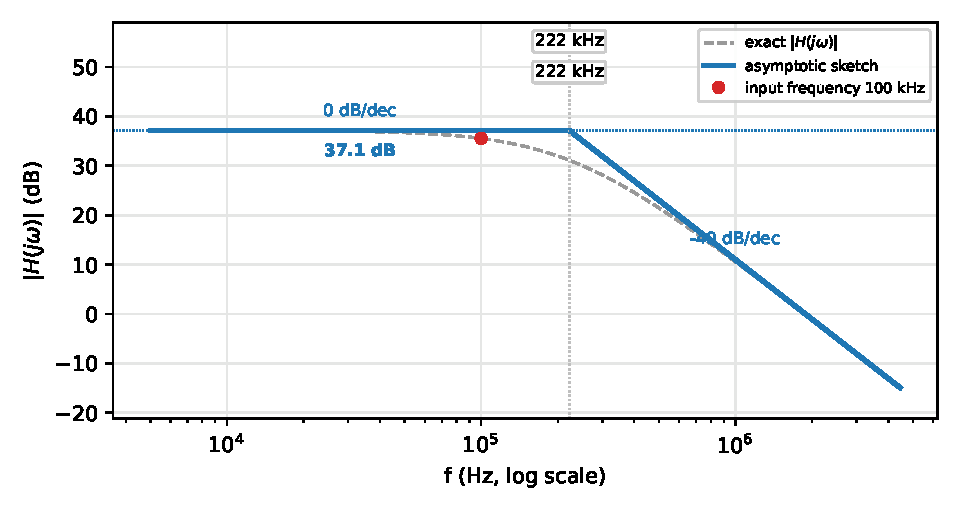
\includegraphics[width=0.78\linewidth,height=6.5cm,keepaspectratio]{p07_bode}\end{center}

{\small Blue: the straight-line sketch you are expected to draw. Dashed grey: the exact curve (about 3\,dB below the corner of an isolated pole). Red dot: the input frequency of Step 7.}
\solstep{7}{Steady-state output}The input is $V_i(t) = 0.01\sin\left(2\pi\cdot 10^{5}\,t\right)$, so $\omega_{in} = 2\pi\cdot 10^{5} = 6.28\times 10^{5}$\,rad/s. Put $s=j\omega_{in}$ in each factor (tool T5): magnitudes multiply, angles add.
{\small Rules: $\left|\frac{s}{s+p}\right| = \frac{\omega}{\sqrt{\omega^2+p^2}}$, $\angle = \frac{\pi}{2}-\tan^{-1}\frac{\omega}{p}$;\quad $\left|\frac{1}{1+s/p}\right| = \frac{1}{\sqrt{1+(\omega/p)^2}}$, $\angle = -\tan^{-1}\frac{\omega}{p}$;\quad $\left|1+\frac{s}{z}\right| = \sqrt{1+(\omega/z)^2}$, $\angle = \tan^{-1}\frac{\omega}{z}$;\quad a negative $K$ adds $-\pi$.}
\begin{center}\renewcommand{\arraystretch}{1.35}
\begin{tabular}{ccc}
\toprule
factor & magnitude & angle (rad) \\
\midrule
$-72$ & $71.99$ & $-3.14$ \\
$\rule[-1.7em]{0pt}{4em}\dfrac{1}{1+\dfrac{s}{2\pi\cdot 222\mathrm{k}}}$ & $0.9119$ & $-0.423$ \\
$\rule[-1.7em]{0pt}{4em}\dfrac{1}{1+\dfrac{s}{2\pi\cdot 222\mathrm{k}}}$ & $0.9119$ & $-0.423$ \\
\textbf{total} & $\mathbf{59.87}$ (product) & $\mathbf{-3.99}$ (sum) \\
\bottomrule
\end{tabular}\end{center}

\begin{align*}
|H(j\omega_{in})| &= 59.9, \qquad \angle H(j\omega_{in}) = -3.99\ \mathrm{rad} \\
v_{o,ac}(t) &= 59.9\times 0.01\,\sin\left(2\pi\cdot 10^{5}\,t - 3.99\right) = 0.599\,\sin\left(2\pi\cdot 10^{5}\,t - 3.99\right)
\end{align*}

\[
\boxed{V_o(t) = 0.599\,\sin\left(2\pi\cdot 10^{5}\,t - 3.99\right)\ \mathrm{V}}
\]

\begin{ansbox}
$H(s) = -72\,\dfrac{1}{1+\dfrac{s}{2\pi\cdot 222\mathrm{k}}}\,\dfrac{1}{1+\dfrac{s}{2\pi\cdot 222\mathrm{k}}}$\quad (corners: 222 kHz, 222 kHz)\\[4pt]
$V_o(t) = 0.599\,\sin\left(2\pi\cdot 10^{5}\,t - 3.99\right)\ \mathrm{V}$
\end{ansbox}

\newpage
\subsection*{Solution 2D.8 \hfill Medium}
\begin{center}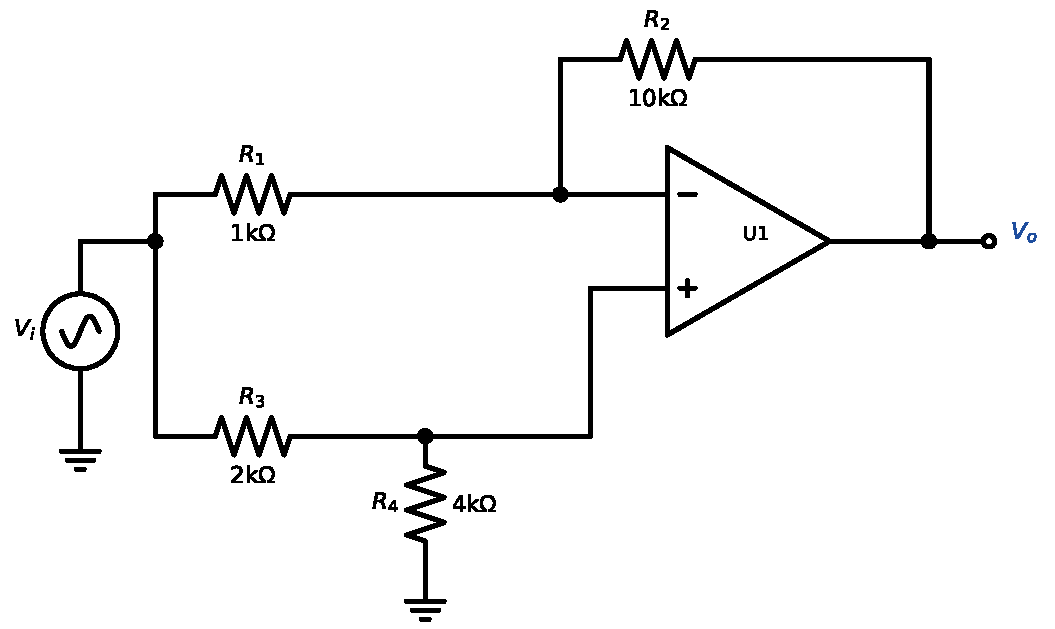
\includegraphics[width=\linewidth,height=5cm,keepaspectratio]{p08_circuit}\end{center}
\solstep{1}{Identify the sources}Independent sources: the AC input $V_i(t)$. No DC source: $V_{o,dc}=0$ and Step 2 is skipped.
\solstep{2}{DC circuit}No DC sources: $V_{o,dc}=0$.
\solstep{3}{Op-amp model}Non-ideal op-amp model (tool T5): $V_{out} = A(s)\,(V_+-V_-)$ with $A(s)=\dfrac{A_0}{1+s/\omega_b}$, $A_0=10^{5}$, $\omega_b = 2\pi\cdot10 = 62.8$\,rad/s, so the unity-gain frequency is $\omega_t = A_0\omega_b = 6.28\times 10^{6}$\,rad/s. The virtual short is \emph{not} used; only ``no current into the inputs'' is still true.

\solstep{4}{Transfer function, op-amp by op-amp}Recipe for each op-amp: write $V_+$ and $V_-$ by superposition of the block input and the op-amp output (each alone is a plain divider): $V_+ = \alpha_+V_{in}$, $V_- = \alpha_-V_{in}+\beta V_{out}$. Then $V_{out} = A(\alpha_+-\alpha_-)V_{in} - A\beta V_{out}$, i.e.\[
\frac{V_{out}}{V_{in}} = \frac{A(\alpha_+-\alpha_-)}{1+A\beta} = \frac{G}{1+\dfrac{1}{A\beta}},\qquad G = \frac{\alpha_+-\alpha_-}{\beta}\ \text{(the ideal gain)}
\]
With $A(s)$ inserted and constant $\alpha,\beta$:\[
\frac{V_{out}}{V_{in}} = G\,\frac{A_0\beta}{1+A_0\beta}\cdot\frac{1}{1+\dfrac{s}{\omega_b(1+A_0\beta)}},\qquad \omega_b(1+A_0\beta)\approx\beta\,\omega_t
\]

\textbf{Block 1 (U1).} (each input is a divider; the $-$ input sees both sources, use superposition)\begin{align*}
V_+ &= \frac{R_{4}}{R_{3}+R_{4}}V_{i} \\
V_- &= \frac{R_{2}}{R_{1}+R_{2}}V_{i} + \frac{R_{1}}{R_{1}+R_{2}}V_{o}
\end{align*}
So $\alpha_+ = 0.6667$, $\alpha_- = 0.9091$, $\beta = 0.09091$: ideal gain $G = \frac{\alpha_+-\alpha_-}{\beta} = -2.667$, $A_0\beta = 9090$.\[
\frac{V_{o}}{V_{i}} = -2.667\cdot\frac{9090}{1+9090}\cdot\frac{1}{1+\dfrac{s}{5.71\times 10^{5}}} = \frac{-2.666}{1+\dfrac{s}{5.71\times 10^{5}}}
\]
(closed-loop bandwidth $\omega_b(1+A_0\beta) = 5.71\times 10^{5}$\,rad/s, $f = 90.9 kHz$; compare $\beta\omega_t = 5.71\times 10^{5}$\,rad/s.)
So:\[
H(s) = \dfrac{-1.52\times 10^{6}}{s + 5.71\times 10^{5}}
\]

\solstep{5}{Standard (Bode-ready) form}Find the roots. Every root $s=-p$ of the denominator is a \emph{pole}, every root $s=-z$ of the numerator is a \emph{zero}; $|p|$ and $|z|$ are the corner frequencies (rad/s).
\begin{itemize}[leftmargin=*,itemsep=2pt]
\item Denominator: $s + 5.71\times 10^{5}$; $s + 5.71\times 10^{5} = 0 \Rightarrow s = -5.71\times 10^{5}$.
\end{itemize}

Factored form (leading coefficient in front):
\[
H(s) = -1.52\times 10^{6}\,\dfrac{1}{(s+5.71\times 10^{5})}
\]

Bode-ready form: rewrite every $(s+p) = p\left(1+\frac{s}{p}\right)$ and $(s+z) = z\left(1+\frac{s}{z}\right)$, and collect all constants into $K$. Then every factor except $K$ is $\approx 1$ inside the pass-band:
\[
H(s) = -2.67\,\dfrac{1}{1+\dfrac{s}{2\pi\cdot 90.9\mathrm{k}}},\qquad K = -2.67
\]

\begin{center}\renewcommand{\arraystretch}{1.35}
\begin{tabular}{cccc}
\toprule
type & $\omega_c$ (rad/s) & $f_c=\omega_c/2\pi$ & slope change \\
\midrule
pole & $5.71\times 10^{5}$ & 90.9 kHz & $-20$ dB/dec \\
\bottomrule
\end{tabular}\end{center}

\solstep{6}{Magnitude Bode plot}Below every corner, all factors are $\approx$ constant: $|H| \approx 2.67$ $= 8.52$\,dB (flat, 0 dB/dec). Then, moving right, each pole bends the line down by 20\,dB/dec and each zero bends it up by 20\,dB/dec (tool T6):
\begin{center}\renewcommand{\arraystretch}{1.35}
\begin{tabular}{lcl}
\toprule
frequency range & slope & asymptote level \\
\midrule
$f<$ 90.9 kHz & $0$ dB/dec (flat) & 8.52 dB at end \\
$f>$ 90.9 kHz & $-20$ dB/dec & 8.52 dB at start \\
\bottomrule
\end{tabular}\end{center}

The flat (pass-band) level is $20\log_{10}|K| = 20\log_{10}2.67 = 8.52$\,dB.
\begin{center}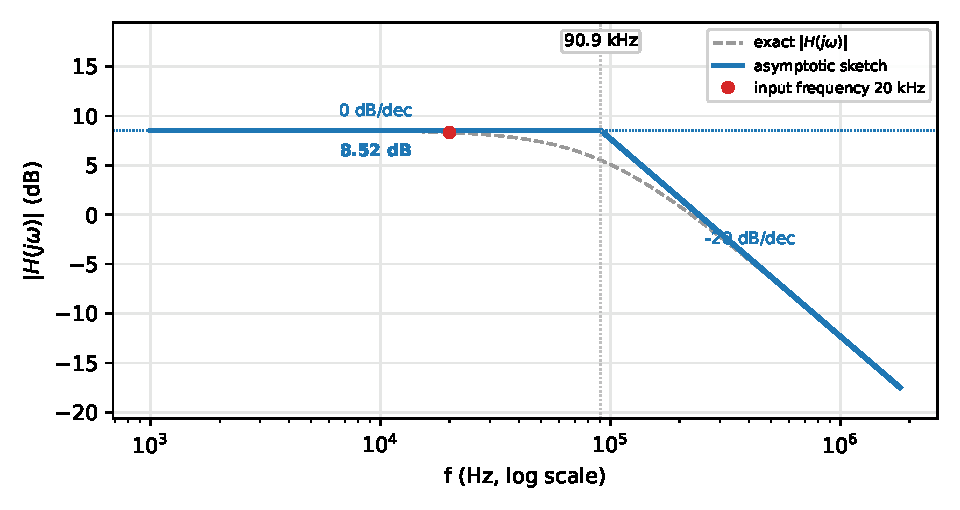
\includegraphics[width=0.78\linewidth,height=6.5cm,keepaspectratio]{p08_bode}\end{center}

{\small Blue: the straight-line sketch you are expected to draw. Dashed grey: the exact curve (about 3\,dB below the corner of an isolated pole). Red dot: the input frequency of Step 7.}
\solstep{7}{Steady-state output}The input is $V_i(t) = 0.1\sin\left(2\pi\cdot 20000\,t\right)$, so $\omega_{in} = 2\pi\cdot 20000 = 1.26\times 10^{5}$\,rad/s. Put $s=j\omega_{in}$ in each factor (tool T5): magnitudes multiply, angles add.
{\small Rules: $\left|\frac{s}{s+p}\right| = \frac{\omega}{\sqrt{\omega^2+p^2}}$, $\angle = \frac{\pi}{2}-\tan^{-1}\frac{\omega}{p}$;\quad $\left|\frac{1}{1+s/p}\right| = \frac{1}{\sqrt{1+(\omega/p)^2}}$, $\angle = -\tan^{-1}\frac{\omega}{p}$;\quad $\left|1+\frac{s}{z}\right| = \sqrt{1+(\omega/z)^2}$, $\angle = \tan^{-1}\frac{\omega}{z}$;\quad a negative $K$ adds $-\pi$.}
\begin{center}\renewcommand{\arraystretch}{1.35}
\begin{tabular}{ccc}
\toprule
factor & magnitude & angle (rad) \\
\midrule
$-2.67$ & $2.666$ & $-3.14$ \\
$\rule[-1.7em]{0pt}{4em}\dfrac{1}{1+\dfrac{s}{2\pi\cdot 90.9\mathrm{k}}}$ & $0.9766$ & $-0.217$ \\
\textbf{total} & $\mathbf{2.604}$ (product) & $\mathbf{-3.36}$ (sum) \\
\bottomrule
\end{tabular}\end{center}

\begin{align*}
|H(j\omega_{in})| &= 2.6, \qquad \angle H(j\omega_{in}) = -3.36\ \mathrm{rad} \\
v_{o,ac}(t) &= 2.6\times 0.1\,\sin\left(2\pi\cdot 20000\,t - 3.36\right) = 0.26\,\sin\left(2\pi\cdot 20000\,t - 3.36\right)
\end{align*}

\[
\boxed{V_o(t) = 0.26\,\sin\left(2\pi\cdot 20000\,t - 3.36\right)\ \mathrm{V}}
\]

\begin{ansbox}
$H(s) = -2.67\,\dfrac{1}{1+\dfrac{s}{2\pi\cdot 90.9\mathrm{k}}}$\quad (corners: 90.9 kHz)\\[4pt]
$V_o(t) = 0.26\,\sin\left(2\pi\cdot 20000\,t - 3.36\right)\ \mathrm{V}$
\end{ansbox}

\newpage
\subsection*{Solution 2D.9 \hfill Medium}
\begin{center}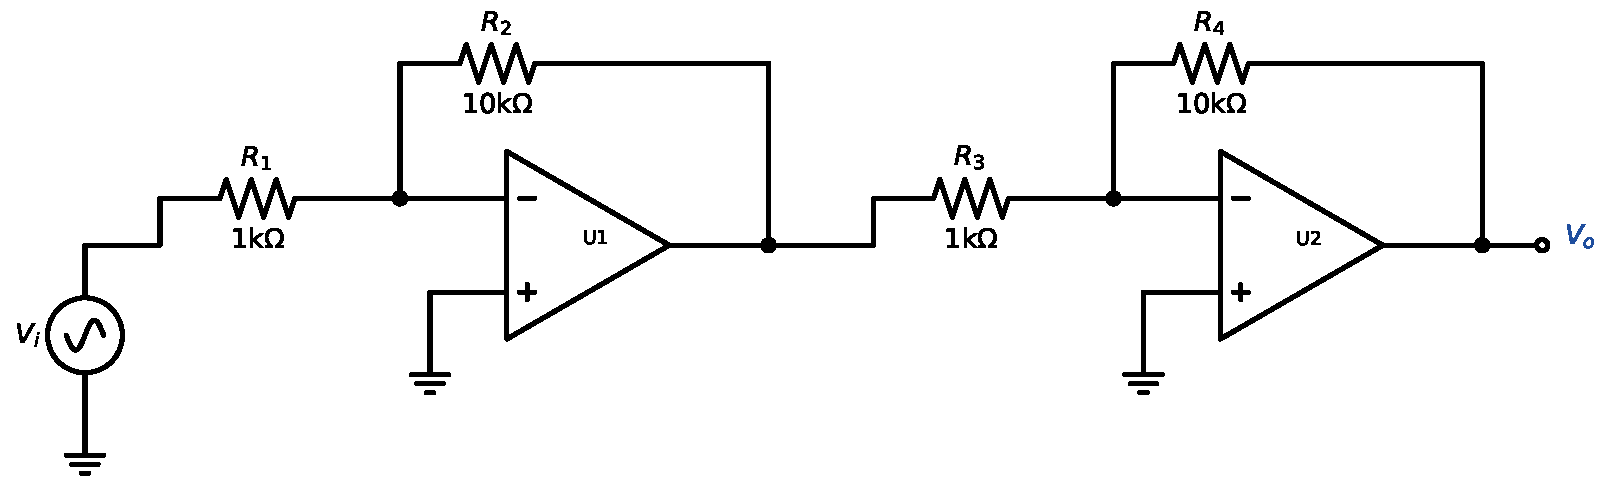
\includegraphics[width=\linewidth,height=5cm,keepaspectratio]{p09_circuit}\end{center}
\solstep{1}{Identify the sources}Independent sources: the AC input $V_i(t)$. No DC source: $V_{o,dc}=0$ and Step 2 is skipped.
\solstep{2}{DC circuit}No DC sources: $V_{o,dc}=0$.
\solstep{3}{Op-amp model}Non-ideal op-amp model (tool T5): $V_{out} = A(s)\,(V_+-V_-)$ with $A(s)=\dfrac{A_0}{1+s/\omega_b}$, $A_0=10^{5}$, $\omega_b = 2\pi\cdot10 = 62.8$\,rad/s, so the unity-gain frequency is $\omega_t = A_0\omega_b = 6.28\times 10^{6}$\,rad/s. The virtual short is \emph{not} used; only ``no current into the inputs'' is still true.

\solstep{4}{Transfer function, op-amp by op-amp}Recipe for each op-amp: write $V_+$ and $V_-$ by superposition of the block input and the op-amp output (each alone is a plain divider): $V_+ = \alpha_+V_{in}$, $V_- = \alpha_-V_{in}+\beta V_{out}$. Then $V_{out} = A(\alpha_+-\alpha_-)V_{in} - A\beta V_{out}$, i.e.\[
\frac{V_{out}}{V_{in}} = \frac{A(\alpha_+-\alpha_-)}{1+A\beta} = \frac{G}{1+\dfrac{1}{A\beta}},\qquad G = \frac{\alpha_+-\alpha_-}{\beta}\ \text{(the ideal gain)}
\]
With $A(s)$ inserted and constant $\alpha,\beta$:\[
\frac{V_{out}}{V_{in}} = G\,\frac{A_0\beta}{1+A_0\beta}\cdot\frac{1}{1+\dfrac{s}{\omega_b(1+A_0\beta)}},\qquad \omega_b(1+A_0\beta)\approx\beta\,\omega_t
\]

\textbf{Block 1 (U1).} (superposition: $V_{i}$ alone with $V_{o1}=0$ gives a divider $R_{1}$--$R_{2}$, and vice versa)\begin{align*}
V_+ &= 0 \quad(\text{grounded}) \\
V_- &= \frac{R_{2}}{R_{1}+R_{2}}V_{i} + \frac{R_{1}}{R_{1}+R_{2}}V_{o1}
\end{align*}
So $\alpha_+ = 0$, $\alpha_- = 0.9091$, $\beta = 0.09091$: ideal gain $G = \frac{\alpha_+-\alpha_-}{\beta} = -10$, $A_0\beta = 9090$.\[
\frac{V_{o1}}{V_{i}} = -10\cdot\frac{9090}{1+9090}\cdot\frac{1}{1+\dfrac{s}{5.71\times 10^{5}}} = \frac{-9.999}{1+\dfrac{s}{5.71\times 10^{5}}}
\]
(closed-loop bandwidth $\omega_b(1+A_0\beta) = 5.71\times 10^{5}$\,rad/s, $f = 90.9 kHz$; compare $\beta\omega_t = 5.71\times 10^{5}$\,rad/s.)
\textbf{Block 2 (U2).} (superposition: $V_{o1}$ alone with $V_{o}=0$ gives a divider $R_{3}$--$R_{4}$, and vice versa)\begin{align*}
V_+ &= 0 \quad(\text{grounded}) \\
V_- &= \frac{R_{4}}{R_{3}+R_{4}}V_{o1} + \frac{R_{3}}{R_{3}+R_{4}}V_{o}
\end{align*}
So $\alpha_+ = 0$, $\alpha_- = 0.9091$, $\beta = 0.09091$: ideal gain $G = \frac{\alpha_+-\alpha_-}{\beta} = -10$, $A_0\beta = 9090$.\[
\frac{V_{o}}{V_{o1}} = -10\cdot\frac{9090}{1+9090}\cdot\frac{1}{1+\dfrac{s}{5.71\times 10^{5}}} = \frac{-9.999}{1+\dfrac{s}{5.71\times 10^{5}}}
\]
(closed-loop bandwidth $\omega_b(1+A_0\beta) = 5.71\times 10^{5}$\,rad/s, $f = 90.9 kHz$; compare $\beta\omega_t = 5.71\times 10^{5}$\,rad/s.)
Each op-amp output is still an ideal source (it is $A(V_+-V_-)$), so the stages multiply.
Multiply the blocks and simplify:\[
H(s) = \dfrac{3.26\times 10^{13}}{s^{2} + 1.14\times 10^{6}\,s + 3.26\times 10^{11}}
\]

\solstep{5}{Standard (Bode-ready) form}Find the roots. Every root $s=-p$ of the denominator is a \emph{pole}, every root $s=-z$ of the numerator is a \emph{zero}; $|p|$ and $|z|$ are the corner frequencies (rad/s).
\begin{itemize}[leftmargin=*,itemsep=2pt]
\item Denominator: $s^{2} + 1.14\times 10^{6}\,s + 3.26\times 10^{11}$; quadratic formula:\[
s = \frac{-1.14\times 10^{6} \pm \sqrt{(1.14\times 10^{6})^2 - 4(3.26\times 10^{11})}}{2} = \frac{-1.14\times 10^{6} \pm 0}{2} \Rightarrow s = -5.71\times 10^{5},\ -5.71\times 10^{5}
\]

\end{itemize}

Factored form (leading coefficient in front):
\[
H(s) = 3.26\times 10^{13}\,\dfrac{1}{(s+5.71\times 10^{5})(s+5.71\times 10^{5})}
\]

Bode-ready form: rewrite every $(s+p) = p\left(1+\frac{s}{p}\right)$ and $(s+z) = z\left(1+\frac{s}{z}\right)$, and collect all constants into $K$. Then every factor except $K$ is $\approx 1$ inside the pass-band:
\[
H(s) = 100\,\dfrac{1}{1+\dfrac{s}{2\pi\cdot 90.9\mathrm{k}}}\,\dfrac{1}{1+\dfrac{s}{2\pi\cdot 90.9\mathrm{k}}},\qquad K = 100
\]

\begin{center}\renewcommand{\arraystretch}{1.35}
\begin{tabular}{cccc}
\toprule
type & $\omega_c$ (rad/s) & $f_c=\omega_c/2\pi$ & slope change \\
\midrule
pole & $5.71\times 10^{5}$ & 90.9 kHz & $-20$ dB/dec \\
pole & $5.71\times 10^{5}$ & 90.9 kHz & $-20$ dB/dec \\
\bottomrule
\end{tabular}\end{center}

\solstep{6}{Magnitude Bode plot}Below every corner, all factors are $\approx$ constant: $|H| \approx 100$ $= 40$\,dB (flat, 0 dB/dec). Then, moving right, each pole bends the line down by 20\,dB/dec and each zero bends it up by 20\,dB/dec (tool T6):
\begin{center}\renewcommand{\arraystretch}{1.35}
\begin{tabular}{lcl}
\toprule
frequency range & slope & asymptote level \\
\midrule
$f<$ 90.9 kHz & $0$ dB/dec (flat) & 40 dB at end \\
90.9 kHz -- 90.9 kHz & $-20$ dB/dec & 40 dB at start, 40 dB at end \\
$f>$ 90.9 kHz & $-40$ dB/dec & 40 dB at start \\
\bottomrule
\end{tabular}\end{center}

The flat (pass-band) level is $20\log_{10}|K| = 20\log_{10}100 = 40$\,dB.
\begin{center}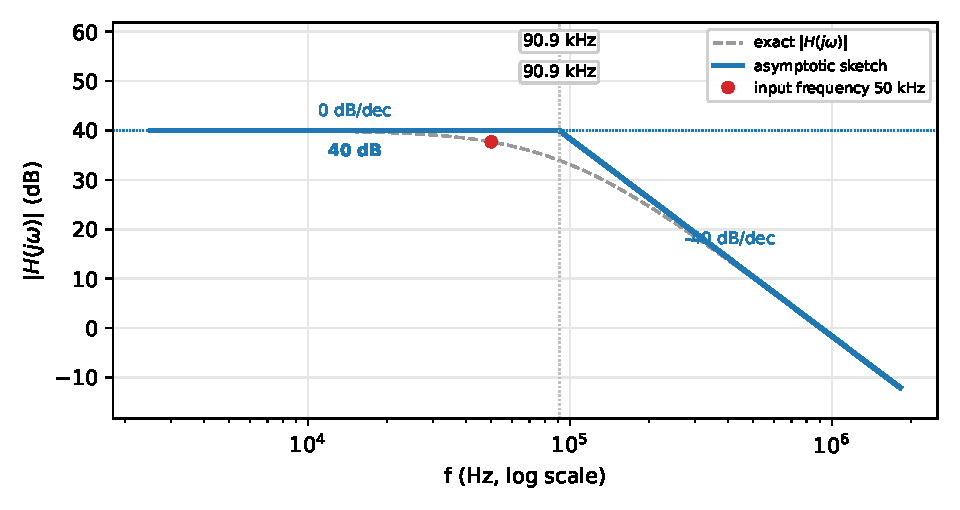
\includegraphics[width=0.78\linewidth,height=6.5cm,keepaspectratio]{p09_bode}\end{center}

{\small Blue: the straight-line sketch you are expected to draw. Dashed grey: the exact curve (about 3\,dB below the corner of an isolated pole). Red dot: the input frequency of Step 7.}
\solstep{7}{Steady-state output}The input is $V_i(t) = 0.01\sin\left(2\pi\cdot 50000\,t\right)$, so $\omega_{in} = 2\pi\cdot 50000 = 3.14\times 10^{5}$\,rad/s. Put $s=j\omega_{in}$ in each factor (tool T5): magnitudes multiply, angles add.
{\small Rules: $\left|\frac{s}{s+p}\right| = \frac{\omega}{\sqrt{\omega^2+p^2}}$, $\angle = \frac{\pi}{2}-\tan^{-1}\frac{\omega}{p}$;\quad $\left|\frac{1}{1+s/p}\right| = \frac{1}{\sqrt{1+(\omega/p)^2}}$, $\angle = -\tan^{-1}\frac{\omega}{p}$;\quad $\left|1+\frac{s}{z}\right| = \sqrt{1+(\omega/z)^2}$, $\angle = \tan^{-1}\frac{\omega}{z}$;\quad a negative $K$ adds $-\pi$.}
\begin{center}\renewcommand{\arraystretch}{1.35}
\begin{tabular}{ccc}
\toprule
factor & magnitude & angle (rad) \\
\midrule
$100$ & $99.98$ & $0$ \\
$\rule[-1.7em]{0pt}{4em}\dfrac{1}{1+\dfrac{s}{2\pi\cdot 90.9\mathrm{k}}}$ & $0.8762$ & $-0.503$ \\
$\rule[-1.7em]{0pt}{4em}\dfrac{1}{1+\dfrac{s}{2\pi\cdot 90.9\mathrm{k}}}$ & $0.8762$ & $-0.503$ \\
\textbf{total} & $\mathbf{76.76}$ (product) & $\mathbf{-1.01}$ (sum) \\
\bottomrule
\end{tabular}\end{center}

\begin{align*}
|H(j\omega_{in})| &= 76.8, \qquad \angle H(j\omega_{in}) = -1.01\ \mathrm{rad} \\
v_{o,ac}(t) &= 76.8\times 0.01\,\sin\left(2\pi\cdot 50000\,t - 1.01\right) = 0.768\,\sin\left(2\pi\cdot 50000\,t - 1.01\right)
\end{align*}

\[
\boxed{V_o(t) = 0.768\,\sin\left(2\pi\cdot 50000\,t - 1.01\right)\ \mathrm{V}}
\]

\begin{ansbox}
$H(s) = 100\,\dfrac{1}{1+\dfrac{s}{2\pi\cdot 90.9\mathrm{k}}}\,\dfrac{1}{1+\dfrac{s}{2\pi\cdot 90.9\mathrm{k}}}$\quad (corners: 90.9 kHz, 90.9 kHz)\\[4pt]
$V_o(t) = 0.768\,\sin\left(2\pi\cdot 50000\,t - 1.01\right)\ \mathrm{V}$
\end{ansbox}

\newpage
\subsection*{Solution 2D.10 \hfill Medium}
\begin{center}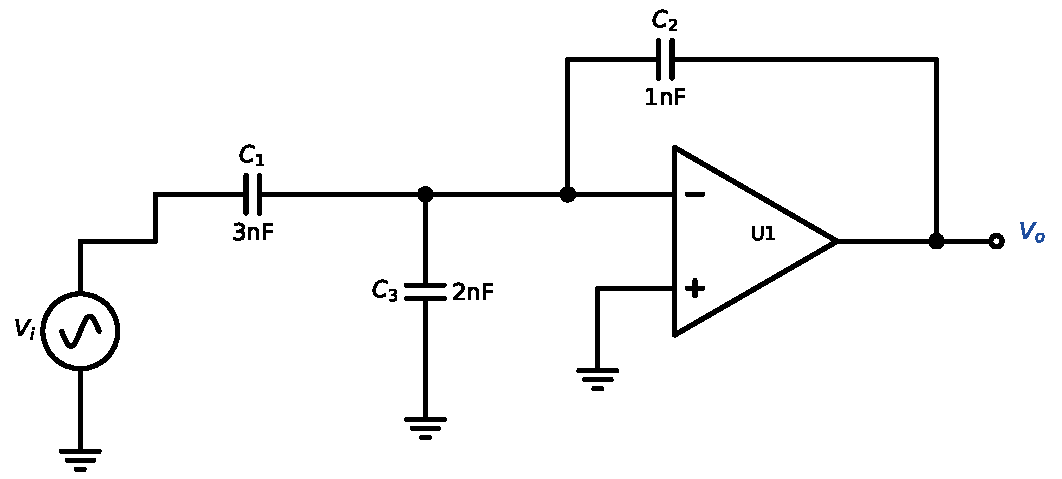
\includegraphics[width=\linewidth,height=5cm,keepaspectratio]{p10_circuit}\end{center}
\solstep{1}{Identify the sources}Independent sources: the AC input $V_i(t)$. No DC source: $V_{o,dc}=0$ and Step 2 is skipped.
\solstep{2}{DC circuit}No DC sources: $V_{o,dc}=0$.
\solstep{3}{Op-amp model}Non-ideal op-amp model (tool T5): $V_{out} = A(s)\,(V_+-V_-)$ with $A(s)=\dfrac{A_0}{1+s/\omega_b}$, $A_0=10^{5}$, $\omega_b = 2\pi\cdot30 = 188$\,rad/s, so the unity-gain frequency is $\omega_t = A_0\omega_b = 1.88\times 10^{7}$\,rad/s. The virtual short is \emph{not} used; only ``no current into the inputs'' is still true.

\solstep{4}{Transfer function, op-amp by op-amp}Recipe for each op-amp: write $V_+$ and $V_-$ by superposition of the block input and the op-amp output (each alone is a plain divider): $V_+ = \alpha_+V_{in}$, $V_- = \alpha_-V_{in}+\beta V_{out}$. Then $V_{out} = A(\alpha_+-\alpha_-)V_{in} - A\beta V_{out}$, i.e.\[
\frac{V_{out}}{V_{in}} = \frac{A(\alpha_+-\alpha_-)}{1+A\beta} = \frac{G}{1+\dfrac{1}{A\beta}},\qquad G = \frac{\alpha_+-\alpha_-}{\beta}\ \text{(the ideal gain)}
\]
With $A(s)$ inserted and constant $\alpha,\beta$:\[
\frac{V_{out}}{V_{in}} = G\,\frac{A_0\beta}{1+A_0\beta}\cdot\frac{1}{1+\dfrac{s}{\omega_b(1+A_0\beta)}},\qquad \omega_b(1+A_0\beta)\approx\beta\,\omega_t
\]

\textbf{Block 1 (U1).} (superposition: with $V_{o}=0$, $\frac{1}{sC_{2}}$ and $\frac{1}{sC_{3}}$ are in parallel from the $-$ input to ground; with $V_{i}=0$, $\frac{1}{sC_{1}}$ and $\frac{1}{sC_{3}}$ are. $\frac{1}{sC_{3}}$ matters now, because $V_-$ is no longer forced to 0.)\begin{align*}
V_+ &= 0 \quad(\text{grounded}) \\
V_- &= \frac{\frac{1}{sC_{2}}\parallel \frac{1}{sC_{3}}}{\frac{1}{sC_{1}}+\frac{1}{sC_{2}}\parallel \frac{1}{sC_{3}}}V_{i} + \frac{\frac{1}{sC_{1}}\parallel \frac{1}{sC_{3}}}{\frac{1}{sC_{2}}+\frac{1}{sC_{1}}\parallel \frac{1}{sC_{3}}}V_{o}
\end{align*}
(Only capacitors: every impedance is $\frac{1}{sC}$, so in each ratio the $s$ cancels, e.g. $\frac{1/(sC_a)}{1/(sC_a)+1/(sC_b)} = \frac{C_b}{C_a+C_b}$, and $\frac{1}{sC_a}\parallel\frac{1}{sC_b} = \frac{1}{s(C_a+C_b)}$.) So $\alpha_+ = 0$, $\alpha_- = 0.5$, $\beta = 0.1667$: ideal gain $G = \frac{\alpha_+-\alpha_-}{\beta} = -3$, $A_0\beta = 16700$.\[
\frac{V_{o}}{V_{i}} = -3\cdot\frac{16700}{1+16700}\cdot\frac{1}{1+\dfrac{s}{3.14\times 10^{6}}} = \frac{-3}{1+\dfrac{s}{3.14\times 10^{6}}}
\]
(closed-loop bandwidth $\omega_b(1+A_0\beta) = 3.14\times 10^{6}$\,rad/s, $f = 500 kHz$; compare $\beta\omega_t = 3.14\times 10^{6}$\,rad/s.)
So:\[
H(s) = \dfrac{-9.42\times 10^{6}}{s + 3.14\times 10^{6}}
\]

\solstep{5}{Standard (Bode-ready) form}Find the roots. Every root $s=-p$ of the denominator is a \emph{pole}, every root $s=-z$ of the numerator is a \emph{zero}; $|p|$ and $|z|$ are the corner frequencies (rad/s).
\begin{itemize}[leftmargin=*,itemsep=2pt]
\item Denominator: $s + 3.14\times 10^{6}$; $s + 3.14\times 10^{6} = 0 \Rightarrow s = -3.14\times 10^{6}$.
\end{itemize}

Factored form (leading coefficient in front):
\[
H(s) = -9.42\times 10^{6}\,\dfrac{1}{(s+3.14\times 10^{6})}
\]

Bode-ready form: rewrite every $(s+p) = p\left(1+\frac{s}{p}\right)$ and $(s+z) = z\left(1+\frac{s}{z}\right)$, and collect all constants into $K$. Then every factor except $K$ is $\approx 1$ inside the pass-band:
\[
H(s) = -3\,\dfrac{1}{1+\dfrac{s}{2\pi\cdot 500\mathrm{k}}},\qquad K = -3
\]

\begin{center}\renewcommand{\arraystretch}{1.35}
\begin{tabular}{cccc}
\toprule
type & $\omega_c$ (rad/s) & $f_c=\omega_c/2\pi$ & slope change \\
\midrule
pole & $3.14\times 10^{6}$ & 500 kHz & $-20$ dB/dec \\
\bottomrule
\end{tabular}\end{center}

\solstep{6}{Magnitude Bode plot}Below every corner, all factors are $\approx$ constant: $|H| \approx 3$ $= 9.54$\,dB (flat, 0 dB/dec). Then, moving right, each pole bends the line down by 20\,dB/dec and each zero bends it up by 20\,dB/dec (tool T6):
\begin{center}\renewcommand{\arraystretch}{1.35}
\begin{tabular}{lcl}
\toprule
frequency range & slope & asymptote level \\
\midrule
$f<$ 500 kHz & $0$ dB/dec (flat) & 9.54 dB at end \\
$f>$ 500 kHz & $-20$ dB/dec & 9.54 dB at start \\
\bottomrule
\end{tabular}\end{center}

The flat (pass-band) level is $20\log_{10}|K| = 20\log_{10}3 = 9.54$\,dB.
\begin{center}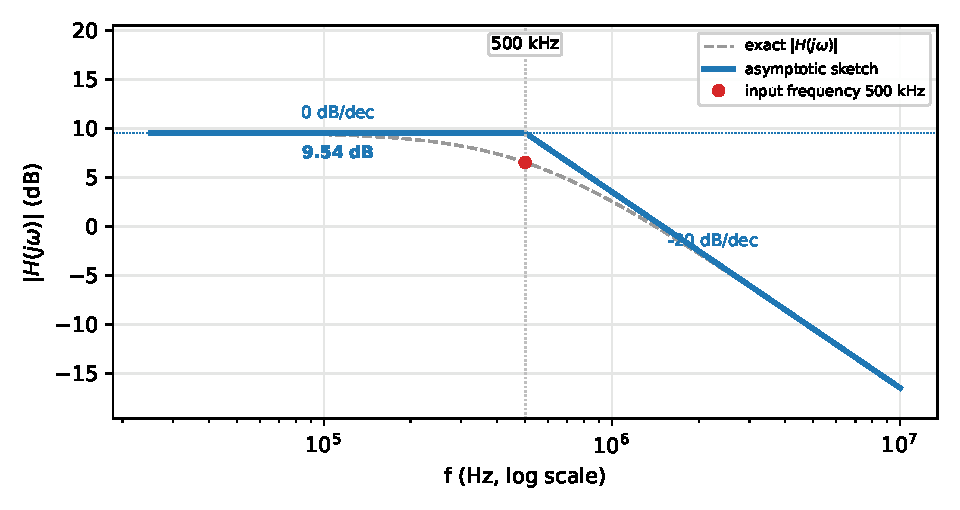
\includegraphics[width=0.78\linewidth,height=6.5cm,keepaspectratio]{p10_bode}\end{center}

{\small Blue: the straight-line sketch you are expected to draw. Dashed grey: the exact curve (about 3\,dB below the corner of an isolated pole). Red dot: the input frequency of Step 7.}
\solstep{7}{Steady-state output}The input is $V_i(t) = 0.05\sin\left(2\pi\cdot 5\times 10^{5}\,t\right)$, so $\omega_{in} = 2\pi\cdot 5\times 10^{5} = 3.14\times 10^{6}$\,rad/s. Put $s=j\omega_{in}$ in each factor (tool T5): magnitudes multiply, angles add.
{\small Rules: $\left|\frac{s}{s+p}\right| = \frac{\omega}{\sqrt{\omega^2+p^2}}$, $\angle = \frac{\pi}{2}-\tan^{-1}\frac{\omega}{p}$;\quad $\left|\frac{1}{1+s/p}\right| = \frac{1}{\sqrt{1+(\omega/p)^2}}$, $\angle = -\tan^{-1}\frac{\omega}{p}$;\quad $\left|1+\frac{s}{z}\right| = \sqrt{1+(\omega/z)^2}$, $\angle = \tan^{-1}\frac{\omega}{z}$;\quad a negative $K$ adds $-\pi$.}
\begin{center}\renewcommand{\arraystretch}{1.35}
\begin{tabular}{ccc}
\toprule
factor & magnitude & angle (rad) \\
\midrule
$-3$ & $3$ & $-3.14$ \\
$\rule[-1.7em]{0pt}{4em}\dfrac{1}{1+\dfrac{s}{2\pi\cdot 500\mathrm{k}}}$ & $0.7071$ & $-0.785$ \\
\textbf{total} & $\mathbf{2.121}$ (product) & $\mathbf{-3.93}$ (sum) \\
\bottomrule
\end{tabular}\end{center}

\begin{align*}
|H(j\omega_{in})| &= 2.12, \qquad \angle H(j\omega_{in}) = -3.93\ \mathrm{rad} \\
v_{o,ac}(t) &= 2.12\times 0.05\,\sin\left(2\pi\cdot 5\times 10^{5}\,t - 3.93\right) = 0.106\,\sin\left(2\pi\cdot 5\times 10^{5}\,t - 3.93\right)
\end{align*}

\[
\boxed{V_o(t) = 0.106\,\sin\left(2\pi\cdot 5\times 10^{5}\,t - 3.93\right)\ \mathrm{V}}
\]

\begin{ansbox}
$H(s) = -3\,\dfrac{1}{1+\dfrac{s}{2\pi\cdot 500\mathrm{k}}}$\quad (corners: 500 kHz)\\[4pt]
$V_o(t) = 0.106\,\sin\left(2\pi\cdot 5\times 10^{5}\,t - 3.93\right)\ \mathrm{V}$
\end{ansbox}

\newpage
\subsection*{Solution 2D.11 \hfill Medium}
\begin{center}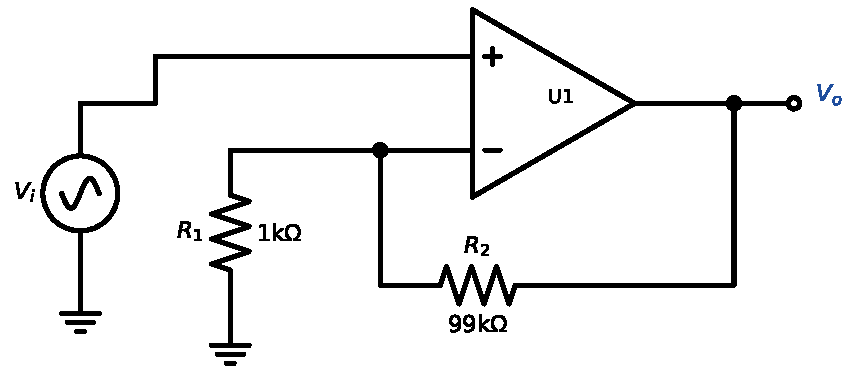
\includegraphics[width=\linewidth,height=5cm,keepaspectratio]{p11_circuit}\end{center}
\solstep{1}{Identify the sources}Independent sources: the AC input $V_i(t)$. No DC source: $V_{o,dc}=0$ and Step 2 is skipped.
\solstep{2}{DC circuit}No DC sources: $V_{o,dc}=0$.
\solstep{3}{Op-amp model}Non-ideal op-amp model (tool T5): $V_{out} = A(s)\,(V_+-V_-)$ with $A(s)=\dfrac{A_0}{1+s/\omega_b}$, $A_0=10^{5}$, $\omega_b = 2\pi\cdot10 = 62.8$\,rad/s, so the unity-gain frequency is $\omega_t = A_0\omega_b = 6.28\times 10^{6}$\,rad/s. The virtual short is \emph{not} used; only ``no current into the inputs'' is still true.

\solstep{4}{Transfer function, op-amp by op-amp}Recipe for each op-amp: write $V_+$ and $V_-$ by superposition of the block input and the op-amp output (each alone is a plain divider): $V_+ = \alpha_+V_{in}$, $V_- = \alpha_-V_{in}+\beta V_{out}$. Then $V_{out} = A(\alpha_+-\alpha_-)V_{in} - A\beta V_{out}$, i.e.\[
\frac{V_{out}}{V_{in}} = \frac{A(\alpha_+-\alpha_-)}{1+A\beta} = \frac{G}{1+\dfrac{1}{A\beta}},\qquad G = \frac{\alpha_+-\alpha_-}{\beta}\ \text{(the ideal gain)}
\]
With $A(s)$ inserted and constant $\alpha,\beta$:\[
\frac{V_{out}}{V_{in}} = G\,\frac{A_0\beta}{1+A_0\beta}\cdot\frac{1}{1+\dfrac{s}{\omega_b(1+A_0\beta)}},\qquad \omega_b(1+A_0\beta)\approx\beta\,\omega_t
\]

\textbf{Block 1 (U1).} (no current enters either input, so both are plain dividers)\begin{align*}
V_+ &= V_{i} \\
V_- &= \frac{R_{1}}{R_{1}+R_{2}}V_{o}
\end{align*}
So $\alpha_+ = 1$, $\alpha_- = 0$, $\beta = 0.01$: ideal gain $G = \frac{\alpha_+-\alpha_-}{\beta} = 100$, $A_0\beta = 1000$.\[
\frac{V_{o}}{V_{i}} = 100\cdot\frac{1000}{1+1000}\cdot\frac{1}{1+\dfrac{s}{62900}} = \frac{99.9}{1+\dfrac{s}{62900}}
\]
(closed-loop bandwidth $\omega_b(1+A_0\beta) = 62900$\,rad/s, $f = 10 kHz$; compare $\beta\omega_t = 62800$\,rad/s.)
So:\[
H(s) = \dfrac{6.28\times 10^{6}}{s + 62900}
\]

\solstep{5}{Standard (Bode-ready) form}Find the roots. Every root $s=-p$ of the denominator is a \emph{pole}, every root $s=-z$ of the numerator is a \emph{zero}; $|p|$ and $|z|$ are the corner frequencies (rad/s).
\begin{itemize}[leftmargin=*,itemsep=2pt]
\item Denominator: $s + 62900$; $s + 62900 = 0 \Rightarrow s = -62900$.
\end{itemize}

Factored form (leading coefficient in front):
\[
H(s) = 6.28\times 10^{6}\,\dfrac{1}{(s+62900)}
\]

Bode-ready form: rewrite every $(s+p) = p\left(1+\frac{s}{p}\right)$ and $(s+z) = z\left(1+\frac{s}{z}\right)$, and collect all constants into $K$. Then every factor except $K$ is $\approx 1$ inside the pass-band:
\[
H(s) = 99.9\,\dfrac{1}{1+\dfrac{s}{2\pi\cdot 10\mathrm{k}}},\qquad K = 99.9
\]

\begin{center}\renewcommand{\arraystretch}{1.35}
\begin{tabular}{cccc}
\toprule
type & $\omega_c$ (rad/s) & $f_c=\omega_c/2\pi$ & slope change \\
\midrule
pole & $62900$ & 10 kHz & $-20$ dB/dec \\
\bottomrule
\end{tabular}\end{center}

\solstep{6}{Magnitude Bode plot}Below every corner, all factors are $\approx$ constant: $|H| \approx 99.9$ $= 40$\,dB (flat, 0 dB/dec). Then, moving right, each pole bends the line down by 20\,dB/dec and each zero bends it up by 20\,dB/dec (tool T6):
\begin{center}\renewcommand{\arraystretch}{1.35}
\begin{tabular}{lcl}
\toprule
frequency range & slope & asymptote level \\
\midrule
$f<$ 10 kHz & $0$ dB/dec (flat) & 40 dB at end \\
$f>$ 10 kHz & $-20$ dB/dec & 40 dB at start \\
\bottomrule
\end{tabular}\end{center}

The flat (pass-band) level is $20\log_{10}|K| = 20\log_{10}99.9 = 40$\,dB.
\begin{center}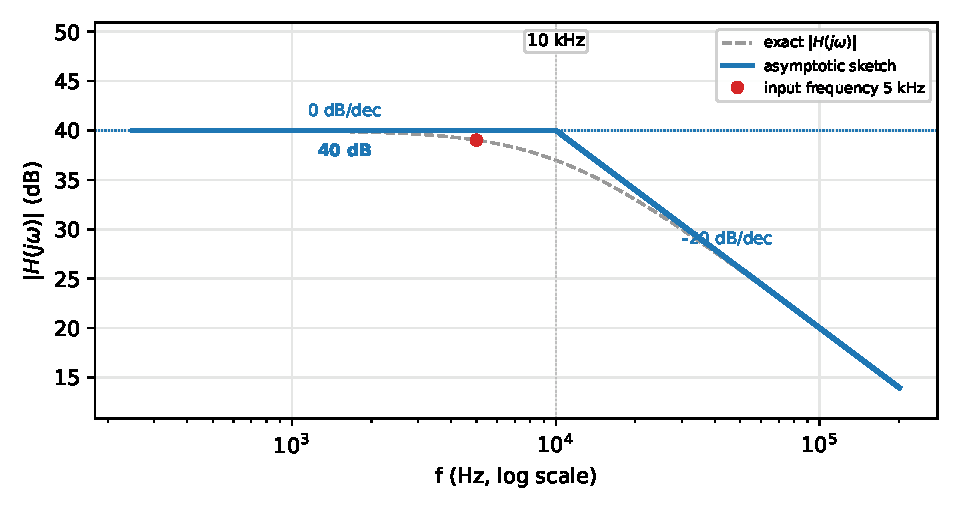
\includegraphics[width=0.78\linewidth,height=6.5cm,keepaspectratio]{p11_bode}\end{center}

{\small Blue: the straight-line sketch you are expected to draw. Dashed grey: the exact curve (about 3\,dB below the corner of an isolated pole). Red dot: the input frequency of Step 7.}
\solstep{7}{Steady-state output}The input is $V_i(t) = 0.01\sin\left(2\pi\cdot 5000\,t\right)$, so $\omega_{in} = 2\pi\cdot 5000 = 31400$\,rad/s. Put $s=j\omega_{in}$ in each factor (tool T5): magnitudes multiply, angles add.
{\small Rules: $\left|\frac{s}{s+p}\right| = \frac{\omega}{\sqrt{\omega^2+p^2}}$, $\angle = \frac{\pi}{2}-\tan^{-1}\frac{\omega}{p}$;\quad $\left|\frac{1}{1+s/p}\right| = \frac{1}{\sqrt{1+(\omega/p)^2}}$, $\angle = -\tan^{-1}\frac{\omega}{p}$;\quad $\left|1+\frac{s}{z}\right| = \sqrt{1+(\omega/z)^2}$, $\angle = \tan^{-1}\frac{\omega}{z}$;\quad a negative $K$ adds $-\pi$.}
\begin{center}\renewcommand{\arraystretch}{1.35}
\begin{tabular}{ccc}
\toprule
factor & magnitude & angle (rad) \\
\midrule
$99.9$ & $99.9$ & $0$ \\
$\rule[-1.7em]{0pt}{4em}\dfrac{1}{1+\dfrac{s}{2\pi\cdot 10\mathrm{k}}}$ & $0.8946$ & $-0.463$ \\
\textbf{total} & $\mathbf{89.37}$ (product) & $\mathbf{-0.463}$ (sum) \\
\bottomrule
\end{tabular}\end{center}

\begin{align*}
|H(j\omega_{in})| &= 89.4, \qquad \angle H(j\omega_{in}) = -0.463\ \mathrm{rad} \\
v_{o,ac}(t) &= 89.4\times 0.01\,\sin\left(2\pi\cdot 5000\,t - 0.463\right) = 0.894\,\sin\left(2\pi\cdot 5000\,t - 0.463\right)
\end{align*}

\[
\boxed{V_o(t) = 0.894\,\sin\left(2\pi\cdot 5000\,t - 0.463\right)\ \mathrm{V}}
\]

\begin{ansbox}
$H(s) = 99.9\,\dfrac{1}{1+\dfrac{s}{2\pi\cdot 10\mathrm{k}}}$\quad (corners: 10 kHz)\\[4pt]
$V_o(t) = 0.894\,\sin\left(2\pi\cdot 5000\,t - 0.463\right)\ \mathrm{V}$
\end{ansbox}

\newpage
\subsection*{Solution 2D.12 \hfill Medium}
\begin{center}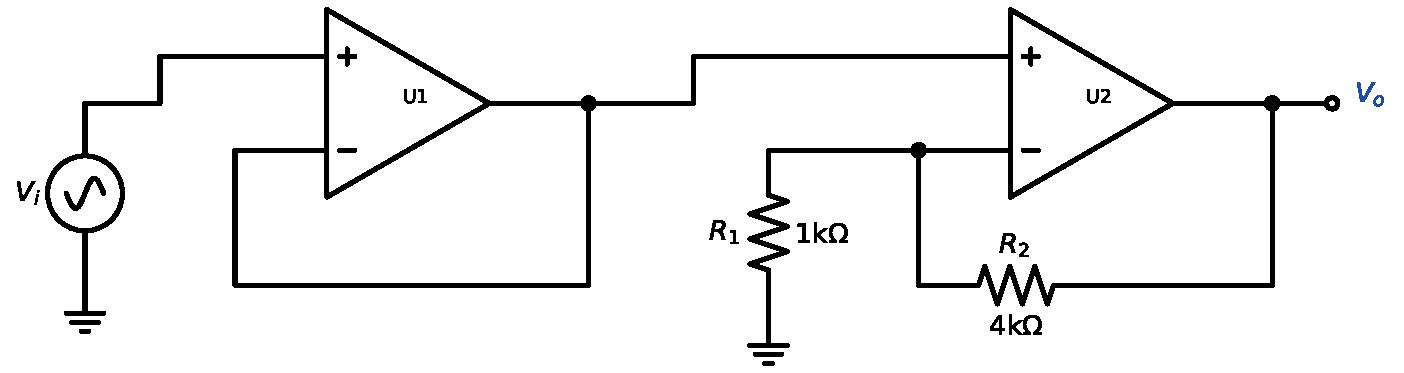
\includegraphics[width=\linewidth,height=5cm,keepaspectratio]{p12_circuit}\end{center}
\solstep{1}{Identify the sources}Independent sources: the AC input $V_i(t)$. No DC source: $V_{o,dc}=0$ and Step 2 is skipped.
\solstep{2}{DC circuit}No DC sources: $V_{o,dc}=0$.
\solstep{3}{Op-amp model}Non-ideal op-amp model (tool T5): $V_{out} = A(s)\,(V_+-V_-)$ with $A(s)=\dfrac{A_0}{1+s/\omega_b}$, $A_0=2\times 10^{5}$, $\omega_b = 2\pi\cdot5 = 31.4$\,rad/s, so the unity-gain frequency is $\omega_t = A_0\omega_b = 6.28\times 10^{6}$\,rad/s. The virtual short is \emph{not} used; only ``no current into the inputs'' is still true.

\solstep{4}{Transfer function, op-amp by op-amp}Recipe for each op-amp: write $V_+$ and $V_-$ by superposition of the block input and the op-amp output (each alone is a plain divider): $V_+ = \alpha_+V_{in}$, $V_- = \alpha_-V_{in}+\beta V_{out}$. Then $V_{out} = A(\alpha_+-\alpha_-)V_{in} - A\beta V_{out}$, i.e.\[
\frac{V_{out}}{V_{in}} = \frac{A(\alpha_+-\alpha_-)}{1+A\beta} = \frac{G}{1+\dfrac{1}{A\beta}},\qquad G = \frac{\alpha_+-\alpha_-}{\beta}\ \text{(the ideal gain)}
\]
With $A(s)$ inserted and constant $\alpha,\beta$:\[
\frac{V_{out}}{V_{in}} = G\,\frac{A_0\beta}{1+A_0\beta}\cdot\frac{1}{1+\dfrac{s}{\omega_b(1+A_0\beta)}},\qquad \omega_b(1+A_0\beta)\approx\beta\,\omega_t
\]

\textbf{Block 1 (U1).} (no current enters either input, so both are plain dividers)\begin{align*}
V_+ &= V_{i} \\
V_- &= V_{o1}
\end{align*}
So $\alpha_+ = 1$, $\alpha_- = 0$, $\beta = 1$: ideal gain $G = \frac{\alpha_+-\alpha_-}{\beta} = 1$, $A_0\beta = 2\times 10^{5}$.\[
\frac{V_{o1}}{V_{i}} = 1\cdot\frac{2\times 10^{5}}{1+2\times 10^{5}}\cdot\frac{1}{1+\dfrac{s}{6.28\times 10^{6}}} = \frac{1}{1+\dfrac{s}{6.28\times 10^{6}}}
\]
(closed-loop bandwidth $\omega_b(1+A_0\beta) = 6.28\times 10^{6}$\,rad/s, $f = 1 MHz$; compare $\beta\omega_t = 6.28\times 10^{6}$\,rad/s.)
\textbf{Block 2 (U2).} (no current enters either input, so both are plain dividers)\begin{align*}
V_+ &= V_{o1} \\
V_- &= \frac{R_{1}}{R_{1}+R_{2}}V_{o}
\end{align*}
So $\alpha_+ = 1$, $\alpha_- = 0$, $\beta = 0.2$: ideal gain $G = \frac{\alpha_+-\alpha_-}{\beta} = 5$, $A_0\beta = 40000$.\[
\frac{V_{o}}{V_{o1}} = 5\cdot\frac{40000}{1+40000}\cdot\frac{1}{1+\dfrac{s}{1.26\times 10^{6}}} = \frac{5}{1+\dfrac{s}{1.26\times 10^{6}}}
\]
(closed-loop bandwidth $\omega_b(1+A_0\beta) = 1.26\times 10^{6}$\,rad/s, $f = 200 kHz$; compare $\beta\omega_t = 1.26\times 10^{6}$\,rad/s.)
Each op-amp output is still an ideal source (it is $A(V_+-V_-)$), so the stages multiply.
Multiply the blocks and simplify:\[
H(s) = \dfrac{3.95\times 10^{13}}{s^{2} + 7.54\times 10^{6}\,s + 7.9\times 10^{12}}
\]

\solstep{5}{Standard (Bode-ready) form}Find the roots. Every root $s=-p$ of the denominator is a \emph{pole}, every root $s=-z$ of the numerator is a \emph{zero}; $|p|$ and $|z|$ are the corner frequencies (rad/s).
\begin{itemize}[leftmargin=*,itemsep=2pt]
\item Denominator: $s^{2} + 7.54\times 10^{6}\,s + 7.9\times 10^{12}$; quadratic formula:\[
s = \frac{-7.54\times 10^{6} \pm \sqrt{(7.54\times 10^{6})^2 - 4(7.9\times 10^{12})}}{2} = \frac{-7.54\times 10^{6} \pm 5.03\times 10^{6}}{2} \Rightarrow s = -1.26\times 10^{6},\ -6.28\times 10^{6}
\]

\end{itemize}

Factored form (leading coefficient in front):
\[
H(s) = 3.95\times 10^{13}\,\dfrac{1}{(s+1.26\times 10^{6})(s+6.28\times 10^{6})}
\]

Bode-ready form: rewrite every $(s+p) = p\left(1+\frac{s}{p}\right)$ and $(s+z) = z\left(1+\frac{s}{z}\right)$, and collect all constants into $K$. Then every factor except $K$ is $\approx 1$ inside the pass-band:
\[
H(s) = 5\,\dfrac{1}{1+\dfrac{s}{2\pi\cdot 200\mathrm{k}}}\,\dfrac{1}{1+\dfrac{s}{2\pi\cdot 1\mathrm{M}}},\qquad K = 5
\]

\begin{center}\renewcommand{\arraystretch}{1.35}
\begin{tabular}{cccc}
\toprule
type & $\omega_c$ (rad/s) & $f_c=\omega_c/2\pi$ & slope change \\
\midrule
pole & $1.26\times 10^{6}$ & 200 kHz & $-20$ dB/dec \\
pole & $6.28\times 10^{6}$ & 1 MHz & $-20$ dB/dec \\
\bottomrule
\end{tabular}\end{center}

\solstep{6}{Magnitude Bode plot}Below every corner, all factors are $\approx$ constant: $|H| \approx 5$ $= 14$\,dB (flat, 0 dB/dec). Then, moving right, each pole bends the line down by 20\,dB/dec and each zero bends it up by 20\,dB/dec (tool T6):
\begin{center}\renewcommand{\arraystretch}{1.35}
\begin{tabular}{lcl}
\toprule
frequency range & slope & asymptote level \\
\midrule
$f<$ 200 kHz & $0$ dB/dec (flat) & 14 dB at end \\
200 kHz -- 1 MHz & $-20$ dB/dec & 14 dB at start, -0.0000869 dB at end \\
$f>$ 1 MHz & $-40$ dB/dec & -0.0000869 dB at start \\
\bottomrule
\end{tabular}\end{center}

The flat (pass-band) level is $20\log_{10}|K| = 20\log_{10}5 = 14$\,dB.
\begin{center}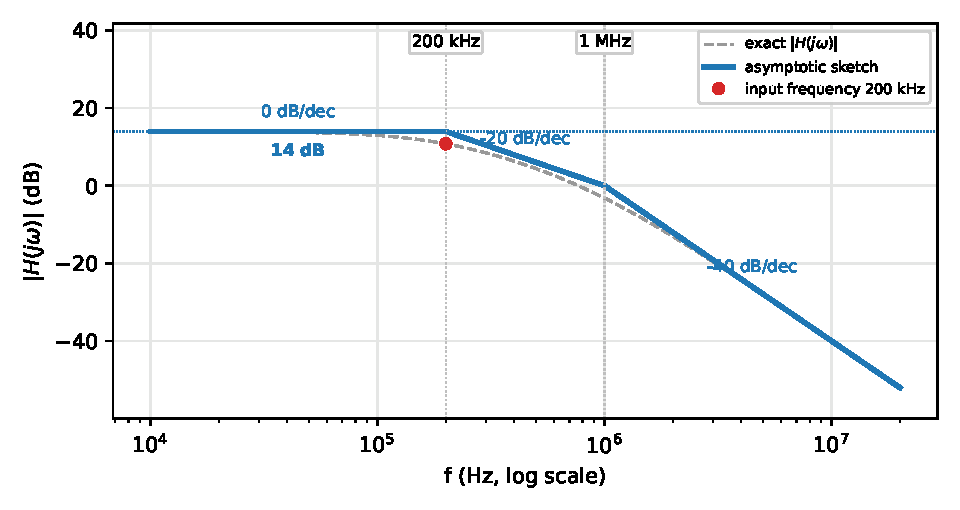
\includegraphics[width=0.78\linewidth,height=6.5cm,keepaspectratio]{p12_bode}\end{center}

{\small Blue: the straight-line sketch you are expected to draw. Dashed grey: the exact curve (about 3\,dB below the corner of an isolated pole). Red dot: the input frequency of Step 7.}
\solstep{7}{Steady-state output}The input is $V_i(t) = 0.1\sin\left(2\pi\cdot 2\times 10^{5}\,t\right)$, so $\omega_{in} = 2\pi\cdot 2\times 10^{5} = 1.26\times 10^{6}$\,rad/s. Put $s=j\omega_{in}$ in each factor (tool T5): magnitudes multiply, angles add.
{\small Rules: $\left|\frac{s}{s+p}\right| = \frac{\omega}{\sqrt{\omega^2+p^2}}$, $\angle = \frac{\pi}{2}-\tan^{-1}\frac{\omega}{p}$;\quad $\left|\frac{1}{1+s/p}\right| = \frac{1}{\sqrt{1+(\omega/p)^2}}$, $\angle = -\tan^{-1}\frac{\omega}{p}$;\quad $\left|1+\frac{s}{z}\right| = \sqrt{1+(\omega/z)^2}$, $\angle = \tan^{-1}\frac{\omega}{z}$;\quad a negative $K$ adds $-\pi$.}
\begin{center}\renewcommand{\arraystretch}{1.35}
\begin{tabular}{ccc}
\toprule
factor & magnitude & angle (rad) \\
\midrule
$5$ & $5$ & $0$ \\
$\rule[-1.7em]{0pt}{4em}\dfrac{1}{1+\dfrac{s}{2\pi\cdot 200\mathrm{k}}}$ & $0.7071$ & $-0.785$ \\
$\rule[-1.7em]{0pt}{4em}\dfrac{1}{1+\dfrac{s}{2\pi\cdot 1\mathrm{M}}}$ & $0.9806$ & $-0.197$ \\
\textbf{total} & $\mathbf{3.467}$ (product) & $\mathbf{-0.983}$ (sum) \\
\bottomrule
\end{tabular}\end{center}

\begin{align*}
|H(j\omega_{in})| &= 3.47, \qquad \angle H(j\omega_{in}) = -0.983\ \mathrm{rad} \\
v_{o,ac}(t) &= 3.47\times 0.1\,\sin\left(2\pi\cdot 2\times 10^{5}\,t - 0.983\right) = 0.347\,\sin\left(2\pi\cdot 2\times 10^{5}\,t - 0.983\right)
\end{align*}

\[
\boxed{V_o(t) = 0.347\,\sin\left(2\pi\cdot 2\times 10^{5}\,t - 0.983\right)\ \mathrm{V}}
\]

\begin{ansbox}
$H(s) = 5\,\dfrac{1}{1+\dfrac{s}{2\pi\cdot 200\mathrm{k}}}\,\dfrac{1}{1+\dfrac{s}{2\pi\cdot 1\mathrm{M}}}$\quad (corners: 200 kHz, 1 MHz)\\[4pt]
$V_o(t) = 0.347\,\sin\left(2\pi\cdot 2\times 10^{5}\,t - 0.983\right)\ \mathrm{V}$
\end{ansbox}

\newpage
\subsection*{Solution 2D.13 \hfill Hard}
\begin{center}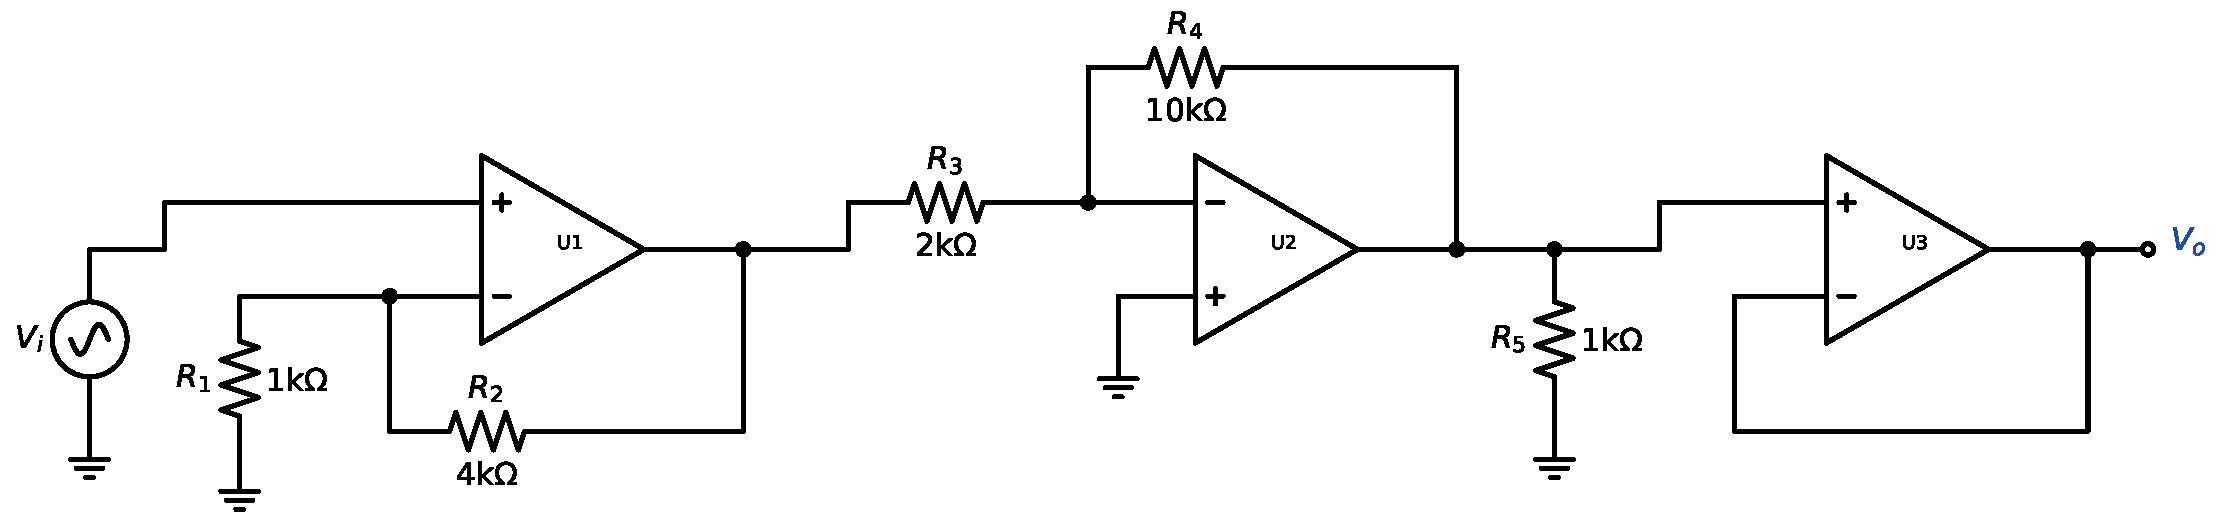
\includegraphics[width=\linewidth,height=5cm,keepaspectratio]{p13_circuit}\end{center}
\solstep{1}{Identify the sources}Independent sources: the AC input $V_i(t)$. No DC source: $V_{o,dc}=0$ and Step 2 is skipped.
\solstep{2}{DC circuit}No DC sources: $V_{o,dc}=0$.
\solstep{3}{Op-amp model}Non-ideal op-amp model (tool T5): $V_{out} = A(s)\,(V_+-V_-)$ with $A(s)=\dfrac{A_0}{1+s/\omega_b}$, $A_0=10^{5}$, $\omega_b = 2\pi\cdot10 = 62.8$\,rad/s, so the unity-gain frequency is $\omega_t = A_0\omega_b = 6.28\times 10^{6}$\,rad/s. The virtual short is \emph{not} used; only ``no current into the inputs'' is still true.

\solstep{4}{Transfer function, op-amp by op-amp}Recipe for each op-amp: write $V_+$ and $V_-$ by superposition of the block input and the op-amp output (each alone is a plain divider): $V_+ = \alpha_+V_{in}$, $V_- = \alpha_-V_{in}+\beta V_{out}$. Then $V_{out} = A(\alpha_+-\alpha_-)V_{in} - A\beta V_{out}$, i.e.\[
\frac{V_{out}}{V_{in}} = \frac{A(\alpha_+-\alpha_-)}{1+A\beta} = \frac{G}{1+\dfrac{1}{A\beta}},\qquad G = \frac{\alpha_+-\alpha_-}{\beta}\ \text{(the ideal gain)}
\]
With $A(s)$ inserted and constant $\alpha,\beta$:\[
\frac{V_{out}}{V_{in}} = G\,\frac{A_0\beta}{1+A_0\beta}\cdot\frac{1}{1+\dfrac{s}{\omega_b(1+A_0\beta)}},\qquad \omega_b(1+A_0\beta)\approx\beta\,\omega_t
\]

The load $R_{5}$ sits on an op-amp output, modelled as the ideal source $A(V_+-V_-)$: it does not change the output voltage and drops out.
\textbf{Block 1 (U1).} (no current enters either input, so both are plain dividers)\begin{align*}
V_+ &= V_{i} \\
V_- &= \frac{R_{1}}{R_{1}+R_{2}}V_{o1}
\end{align*}
So $\alpha_+ = 1$, $\alpha_- = 0$, $\beta = 0.2$: ideal gain $G = \frac{\alpha_+-\alpha_-}{\beta} = 5$, $A_0\beta = 20000$.\[
\frac{V_{o1}}{V_{i}} = 5\cdot\frac{20000}{1+20000}\cdot\frac{1}{1+\dfrac{s}{1.26\times 10^{6}}} = \frac{5}{1+\dfrac{s}{1.26\times 10^{6}}}
\]
(closed-loop bandwidth $\omega_b(1+A_0\beta) = 1.26\times 10^{6}$\,rad/s, $f = 200 kHz$; compare $\beta\omega_t = 1.26\times 10^{6}$\,rad/s.)
\textbf{Block 2 (U2).} (superposition: $V_{o1}$ alone with $V_{o2}=0$ gives a divider $R_{3}$--$R_{4}$, and vice versa)\begin{align*}
V_+ &= 0 \quad(\text{grounded}) \\
V_- &= \frac{R_{4}}{R_{3}+R_{4}}V_{o1} + \frac{R_{3}}{R_{3}+R_{4}}V_{o2}
\end{align*}
So $\alpha_+ = 0$, $\alpha_- = 0.8333$, $\beta = 0.1667$: ideal gain $G = \frac{\alpha_+-\alpha_-}{\beta} = -5$, $A_0\beta = 16700$.\[
\frac{V_{o2}}{V_{o1}} = -5\cdot\frac{16700}{1+16700}\cdot\frac{1}{1+\dfrac{s}{1.05\times 10^{6}}} = \frac{-5}{1+\dfrac{s}{1.05\times 10^{6}}}
\]
(closed-loop bandwidth $\omega_b(1+A_0\beta) = 1.05\times 10^{6}$\,rad/s, $f = 167 kHz$; compare $\beta\omega_t = 1.05\times 10^{6}$\,rad/s.)
\textbf{Block 3 (U3).} (no current enters either input, so both are plain dividers)\begin{align*}
V_+ &= V_{o2} \\
V_- &= V_{o}
\end{align*}
So $\alpha_+ = 1$, $\alpha_- = 0$, $\beta = 1$: ideal gain $G = \frac{\alpha_+-\alpha_-}{\beta} = 1$, $A_0\beta = 10^{5}$.\[
\frac{V_{o}}{V_{o2}} = 1\cdot\frac{10^{5}}{1+10^{5}}\cdot\frac{1}{1+\dfrac{s}{6.28\times 10^{6}}} = \frac{1}{1+\dfrac{s}{6.28\times 10^{6}}}
\]
(closed-loop bandwidth $\omega_b(1+A_0\beta) = 6.28\times 10^{6}$\,rad/s, $f = 1 MHz$; compare $\beta\omega_t = 6.28\times 10^{6}$\,rad/s.)
Each op-amp output is still an ideal source (it is $A(V_+-V_-)$), so the stages multiply.
Multiply the blocks and simplify:\[
H(s) = \dfrac{-2.07\times 10^{20}}{s^{3} + 8.59\times 10^{6}\,s^{2} + 1.58\times 10^{13}\,s + 8.27\times 10^{18}}
\]

\solstep{5}{Standard (Bode-ready) form}Find the roots. Every root $s=-p$ of the denominator is a \emph{pole}, every root $s=-z$ of the numerator is a \emph{zero}; $|p|$ and $|z|$ are the corner frequencies (rad/s).
\begin{itemize}[leftmargin=*,itemsep=2pt]
\item Denominator: $s^{3} + 8.59\times 10^{6}\,s^{2} + 1.58\times 10^{13}\,s + 8.27\times 10^{18}$; this is degree 3: use a calculator's polynomial solver (or \texttt{numpy.roots}) $\Rightarrow s = -1.05\times 10^{6},\ -1.26\times 10^{6},\ -6.28\times 10^{6}$.
\end{itemize}

Factored form (leading coefficient in front):
\[
H(s) = -2.07\times 10^{20}\,\dfrac{1}{(s+1.05\times 10^{6})(s+1.26\times 10^{6})(s+6.28\times 10^{6})}
\]

Bode-ready form: rewrite every $(s+p) = p\left(1+\frac{s}{p}\right)$ and $(s+z) = z\left(1+\frac{s}{z}\right)$, and collect all constants into $K$. Then every factor except $K$ is $\approx 1$ inside the pass-band:
\[
H(s) = -25\,\dfrac{1}{1+\dfrac{s}{2\pi\cdot 167\mathrm{k}}}\,\dfrac{1}{1+\dfrac{s}{2\pi\cdot 200\mathrm{k}}}\,\dfrac{1}{1+\dfrac{s}{2\pi\cdot 1\mathrm{M}}},\qquad K = -25
\]

\begin{center}\renewcommand{\arraystretch}{1.35}
\begin{tabular}{cccc}
\toprule
type & $\omega_c$ (rad/s) & $f_c=\omega_c/2\pi$ & slope change \\
\midrule
pole & $1.05\times 10^{6}$ & 167 kHz & $-20$ dB/dec \\
pole & $1.26\times 10^{6}$ & 200 kHz & $-20$ dB/dec \\
pole & $6.28\times 10^{6}$ & 1 MHz & $-20$ dB/dec \\
\bottomrule
\end{tabular}\end{center}

\solstep{6}{Magnitude Bode plot}Below every corner, all factors are $\approx$ constant: $|H| \approx 25$ $= 28$\,dB (flat, 0 dB/dec). Then, moving right, each pole bends the line down by 20\,dB/dec and each zero bends it up by 20\,dB/dec (tool T6):
\begin{center}\renewcommand{\arraystretch}{1.35}
\begin{tabular}{lcl}
\toprule
frequency range & slope & asymptote level \\
\midrule
$f<$ 167 kHz & $0$ dB/dec (flat) & 28 dB at end \\
167 kHz -- 200 kHz & $-20$ dB/dec & 28 dB at start, 26.4 dB at end \\
200 kHz -- 1 MHz & $-40$ dB/dec & 26.4 dB at start, -1.58 dB at end \\
$f>$ 1 MHz & $-60$ dB/dec & -1.58 dB at start \\
\bottomrule
\end{tabular}\end{center}

The flat (pass-band) level is $20\log_{10}|K| = 20\log_{10}25 = 28$\,dB.
\begin{center}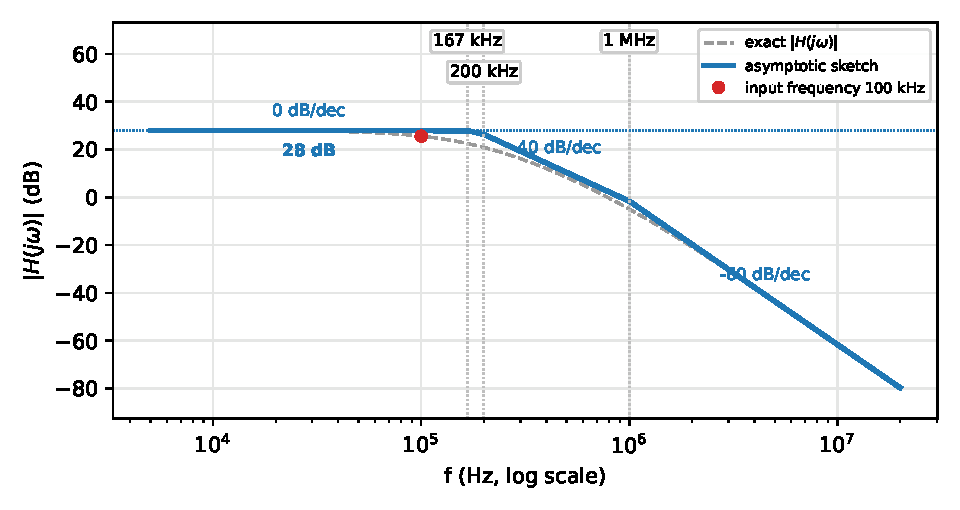
\includegraphics[width=0.78\linewidth,height=6.5cm,keepaspectratio]{p13_bode}\end{center}

{\small Blue: the straight-line sketch you are expected to draw. Dashed grey: the exact curve (about 3\,dB below the corner of an isolated pole). Red dot: the input frequency of Step 7.}
\solstep{7}{Steady-state output}The input is $V_i(t) = 0.02\sin\left(2\pi\cdot 10^{5}\,t\right)$, so $\omega_{in} = 2\pi\cdot 10^{5} = 6.28\times 10^{5}$\,rad/s. Put $s=j\omega_{in}$ in each factor (tool T5): magnitudes multiply, angles add.
{\small Rules: $\left|\frac{s}{s+p}\right| = \frac{\omega}{\sqrt{\omega^2+p^2}}$, $\angle = \frac{\pi}{2}-\tan^{-1}\frac{\omega}{p}$;\quad $\left|\frac{1}{1+s/p}\right| = \frac{1}{\sqrt{1+(\omega/p)^2}}$, $\angle = -\tan^{-1}\frac{\omega}{p}$;\quad $\left|1+\frac{s}{z}\right| = \sqrt{1+(\omega/z)^2}$, $\angle = \tan^{-1}\frac{\omega}{z}$;\quad a negative $K$ adds $-\pi$.}
\begin{center}\renewcommand{\arraystretch}{1.35}
\begin{tabular}{ccc}
\toprule
factor & magnitude & angle (rad) \\
\midrule
$-25$ & $25$ & $-3.14$ \\
$\rule[-1.7em]{0pt}{4em}\dfrac{1}{1+\dfrac{s}{2\pi\cdot 167\mathrm{k}}}$ & $0.8575$ & $-0.54$ \\
$\rule[-1.7em]{0pt}{4em}\dfrac{1}{1+\dfrac{s}{2\pi\cdot 200\mathrm{k}}}$ & $0.8944$ & $-0.464$ \\
$\rule[-1.7em]{0pt}{4em}\dfrac{1}{1+\dfrac{s}{2\pi\cdot 1\mathrm{M}}}$ & $0.995$ & $-0.0997$ \\
\textbf{total} & $\mathbf{19.08}$ (product) & $\mathbf{-4.25}$ (sum) \\
\bottomrule
\end{tabular}\end{center}

\begin{align*}
|H(j\omega_{in})| &= 19.1, \qquad \angle H(j\omega_{in}) = -4.25\ \mathrm{rad} \\
v_{o,ac}(t) &= 19.1\times 0.02\,\sin\left(2\pi\cdot 10^{5}\,t - 4.25\right) = 0.382\,\sin\left(2\pi\cdot 10^{5}\,t - 4.25\right)
\end{align*}

\[
\boxed{V_o(t) = 0.382\,\sin\left(2\pi\cdot 10^{5}\,t - 4.25\right)\ \mathrm{V}}
\]

\begin{ansbox}
$H(s) = -25\,\dfrac{1}{1+\dfrac{s}{2\pi\cdot 167\mathrm{k}}}\,\dfrac{1}{1+\dfrac{s}{2\pi\cdot 200\mathrm{k}}}\,\dfrac{1}{1+\dfrac{s}{2\pi\cdot 1\mathrm{M}}}$\quad (corners: 167 kHz, 200 kHz, 1 MHz)\\[4pt]
$V_o(t) = 0.382\,\sin\left(2\pi\cdot 10^{5}\,t - 4.25\right)\ \mathrm{V}$
\end{ansbox}

\newpage
\subsection*{Solution 2D.14 \hfill Hard}
\begin{center}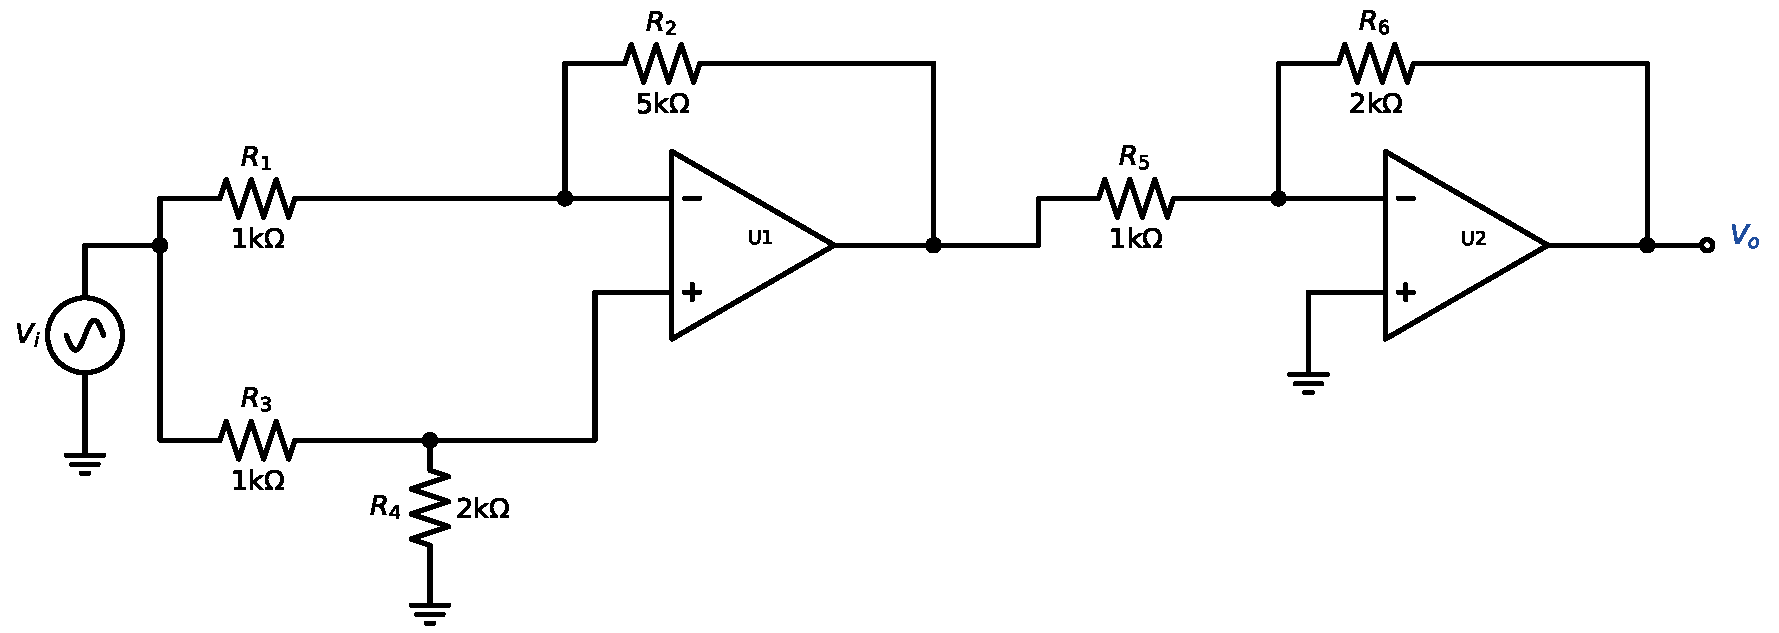
\includegraphics[width=\linewidth,height=5cm,keepaspectratio]{p14_circuit}\end{center}
\solstep{1}{Identify the sources}Independent sources: the AC input $V_i(t)$. No DC source: $V_{o,dc}=0$ and Step 2 is skipped.
\solstep{2}{DC circuit}No DC sources: $V_{o,dc}=0$.
\solstep{3}{Op-amp model}Non-ideal op-amp model (tool T5): $V_{out} = A(s)\,(V_+-V_-)$ with $A(s)=\dfrac{A_0}{1+s/\omega_b}$, $A_0=10^{5}$, $\omega_b = 2\pi\cdot20 = 126$\,rad/s, so the unity-gain frequency is $\omega_t = A_0\omega_b = 1.26\times 10^{7}$\,rad/s. The virtual short is \emph{not} used; only ``no current into the inputs'' is still true.

\solstep{4}{Transfer function, op-amp by op-amp}Recipe for each op-amp: write $V_+$ and $V_-$ by superposition of the block input and the op-amp output (each alone is a plain divider): $V_+ = \alpha_+V_{in}$, $V_- = \alpha_-V_{in}+\beta V_{out}$. Then $V_{out} = A(\alpha_+-\alpha_-)V_{in} - A\beta V_{out}$, i.e.\[
\frac{V_{out}}{V_{in}} = \frac{A(\alpha_+-\alpha_-)}{1+A\beta} = \frac{G}{1+\dfrac{1}{A\beta}},\qquad G = \frac{\alpha_+-\alpha_-}{\beta}\ \text{(the ideal gain)}
\]
With $A(s)$ inserted and constant $\alpha,\beta$:\[
\frac{V_{out}}{V_{in}} = G\,\frac{A_0\beta}{1+A_0\beta}\cdot\frac{1}{1+\dfrac{s}{\omega_b(1+A_0\beta)}},\qquad \omega_b(1+A_0\beta)\approx\beta\,\omega_t
\]

\textbf{Block 1 (U1).} (each input is a divider; the $-$ input sees both sources, use superposition)\begin{align*}
V_+ &= \frac{R_{4}}{R_{3}+R_{4}}V_{i} \\
V_- &= \frac{R_{2}}{R_{1}+R_{2}}V_{i} + \frac{R_{1}}{R_{1}+R_{2}}V_{o1}
\end{align*}
So $\alpha_+ = 0.6667$, $\alpha_- = 0.8333$, $\beta = 0.1667$: ideal gain $G = \frac{\alpha_+-\alpha_-}{\beta} = -1$, $A_0\beta = 16700$.\[
\frac{V_{o1}}{V_{i}} = -1\cdot\frac{16700}{1+16700}\cdot\frac{1}{1+\dfrac{s}{2.09\times 10^{6}}} = \frac{-0.9999}{1+\dfrac{s}{2.09\times 10^{6}}}
\]
(closed-loop bandwidth $\omega_b(1+A_0\beta) = 2.09\times 10^{6}$\,rad/s, $f = 333 kHz$; compare $\beta\omega_t = 2.09\times 10^{6}$\,rad/s.)
\textbf{Block 2 (U2).} (superposition: $V_{o1}$ alone with $V_{o}=0$ gives a divider $R_{5}$--$R_{6}$, and vice versa)\begin{align*}
V_+ &= 0 \quad(\text{grounded}) \\
V_- &= \frac{R_{6}}{R_{5}+R_{6}}V_{o1} + \frac{R_{5}}{R_{5}+R_{6}}V_{o}
\end{align*}
So $\alpha_+ = 0$, $\alpha_- = 0.6667$, $\beta = 0.3333$: ideal gain $G = \frac{\alpha_+-\alpha_-}{\beta} = -2$, $A_0\beta = 33300$.\[
\frac{V_{o}}{V_{o1}} = -2\cdot\frac{33300}{1+33300}\cdot\frac{1}{1+\dfrac{s}{4.19\times 10^{6}}} = \frac{-2}{1+\dfrac{s}{4.19\times 10^{6}}}
\]
(closed-loop bandwidth $\omega_b(1+A_0\beta) = 4.19\times 10^{6}$\,rad/s, $f = 667 kHz$; compare $\beta\omega_t = 4.19\times 10^{6}$\,rad/s.)
Each op-amp output is still an ideal source (it is $A(V_+-V_-)$), so the stages multiply.
Multiply the blocks and simplify:\[
H(s) = \dfrac{1.75\times 10^{13}}{s^{2} + 6.28\times 10^{6}\,s + 8.77\times 10^{12}}
\]

\solstep{5}{Standard (Bode-ready) form}Find the roots. Every root $s=-p$ of the denominator is a \emph{pole}, every root $s=-z$ of the numerator is a \emph{zero}; $|p|$ and $|z|$ are the corner frequencies (rad/s).
\begin{itemize}[leftmargin=*,itemsep=2pt]
\item Denominator: $s^{2} + 6.28\times 10^{6}\,s + 8.77\times 10^{12}$; quadratic formula:\[
s = \frac{-6.28\times 10^{6} \pm \sqrt{(6.28\times 10^{6})^2 - 4(8.77\times 10^{12})}}{2} = \frac{-6.28\times 10^{6} \pm 2.09\times 10^{6}}{2} \Rightarrow s = -2.09\times 10^{6},\ -4.19\times 10^{6}
\]

\end{itemize}

Factored form (leading coefficient in front):
\[
H(s) = 1.75\times 10^{13}\,\dfrac{1}{(s+2.09\times 10^{6})(s+4.19\times 10^{6})}
\]

Bode-ready form: rewrite every $(s+p) = p\left(1+\frac{s}{p}\right)$ and $(s+z) = z\left(1+\frac{s}{z}\right)$, and collect all constants into $K$. Then every factor except $K$ is $\approx 1$ inside the pass-band:
\[
H(s) = 2\,\dfrac{1}{1+\dfrac{s}{2\pi\cdot 333\mathrm{k}}}\,\dfrac{1}{1+\dfrac{s}{2\pi\cdot 667\mathrm{k}}},\qquad K = 2
\]

\begin{center}\renewcommand{\arraystretch}{1.35}
\begin{tabular}{cccc}
\toprule
type & $\omega_c$ (rad/s) & $f_c=\omega_c/2\pi$ & slope change \\
\midrule
pole & $2.09\times 10^{6}$ & 333 kHz & $-20$ dB/dec \\
pole & $4.19\times 10^{6}$ & 667 kHz & $-20$ dB/dec \\
\bottomrule
\end{tabular}\end{center}

\solstep{6}{Magnitude Bode plot}Below every corner, all factors are $\approx$ constant: $|H| \approx 2$ $= 6.02$\,dB (flat, 0 dB/dec). Then, moving right, each pole bends the line down by 20\,dB/dec and each zero bends it up by 20\,dB/dec (tool T6):
\begin{center}\renewcommand{\arraystretch}{1.35}
\begin{tabular}{lcl}
\toprule
frequency range & slope & asymptote level \\
\midrule
$f<$ 333 kHz & $0$ dB/dec (flat) & 6.02 dB at end \\
333 kHz -- 667 kHz & $-20$ dB/dec & 6.02 dB at start, -0.000521 dB at end \\
$f>$ 667 kHz & $-40$ dB/dec & -0.000521 dB at start \\
\bottomrule
\end{tabular}\end{center}

The flat (pass-band) level is $20\log_{10}|K| = 20\log_{10}2 = 6.02$\,dB.
\begin{center}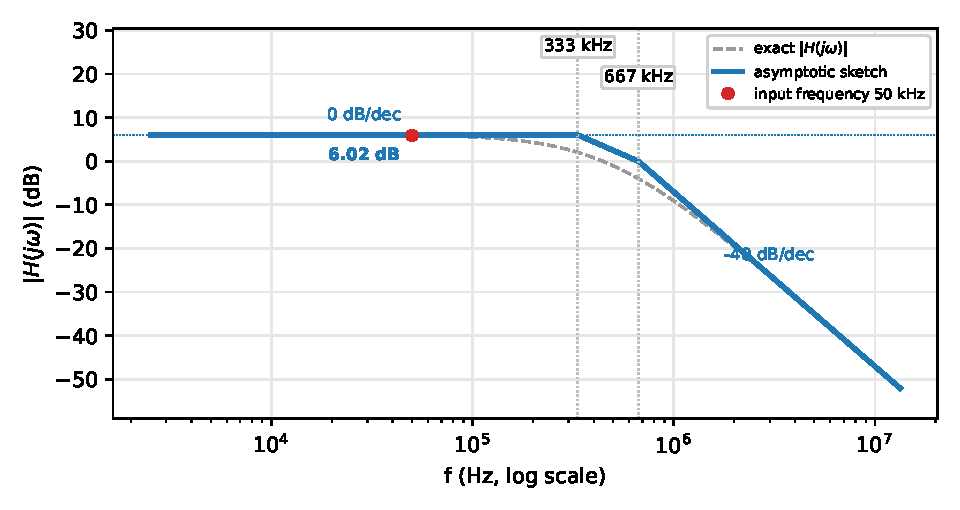
\includegraphics[width=0.78\linewidth,height=6.5cm,keepaspectratio]{p14_bode}\end{center}

{\small Blue: the straight-line sketch you are expected to draw. Dashed grey: the exact curve (about 3\,dB below the corner of an isolated pole). Red dot: the input frequency of Step 7.}
\solstep{7}{Steady-state output}The input is $V_i(t) = 0.05\sin\left(2\pi\cdot 50000\,t+\frac{\pi}{4}\right)$, so $\omega_{in} = 2\pi\cdot 50000 = 3.14\times 10^{5}$\,rad/s. Put $s=j\omega_{in}$ in each factor (tool T5): magnitudes multiply, angles add.
{\small Rules: $\left|\frac{s}{s+p}\right| = \frac{\omega}{\sqrt{\omega^2+p^2}}$, $\angle = \frac{\pi}{2}-\tan^{-1}\frac{\omega}{p}$;\quad $\left|\frac{1}{1+s/p}\right| = \frac{1}{\sqrt{1+(\omega/p)^2}}$, $\angle = -\tan^{-1}\frac{\omega}{p}$;\quad $\left|1+\frac{s}{z}\right| = \sqrt{1+(\omega/z)^2}$, $\angle = \tan^{-1}\frac{\omega}{z}$;\quad a negative $K$ adds $-\pi$.}
\begin{center}\renewcommand{\arraystretch}{1.35}
\begin{tabular}{ccc}
\toprule
factor & magnitude & angle (rad) \\
\midrule
$2$ & $2$ & $0$ \\
$\rule[-1.7em]{0pt}{4em}\dfrac{1}{1+\dfrac{s}{2\pi\cdot 333\mathrm{k}}}$ & $0.9889$ & $-0.149$ \\
$\rule[-1.7em]{0pt}{4em}\dfrac{1}{1+\dfrac{s}{2\pi\cdot 667\mathrm{k}}}$ & $0.9972$ & $-0.0749$ \\
\textbf{total} & $\mathbf{1.972}$ (product) & $\mathbf{-0.224}$ (sum) \\
\bottomrule
\end{tabular}\end{center}

\begin{align*}
|H(j\omega_{in})| &= 1.97, \qquad \angle H(j\omega_{in}) = -0.224\ \mathrm{rad} \\
v_{o,ac}(t) &= 1.97\times 0.05\,\sin\left(2\pi\cdot 50000\,t + 0.562\right) = 0.0986\,\sin\left(2\pi\cdot 50000\,t + 0.562\right)
\end{align*}

(phase: $\theta + \angle H = \frac{\pi}{4} + (-0.224) = 0.562$\,rad.)
\[
\boxed{V_o(t) = 0.0986\,\sin\left(2\pi\cdot 50000\,t + 0.562\right)\ \mathrm{V}}
\]

\begin{ansbox}
$H(s) = 2\,\dfrac{1}{1+\dfrac{s}{2\pi\cdot 333\mathrm{k}}}\,\dfrac{1}{1+\dfrac{s}{2\pi\cdot 667\mathrm{k}}}$\quad (corners: 333 kHz, 667 kHz)\\[4pt]
$V_o(t) = 0.0986\,\sin\left(2\pi\cdot 50000\,t + 0.562\right)\ \mathrm{V}$
\end{ansbox}

\newpage
\subsection*{Solution 2D.15 \hfill Hard}
\begin{center}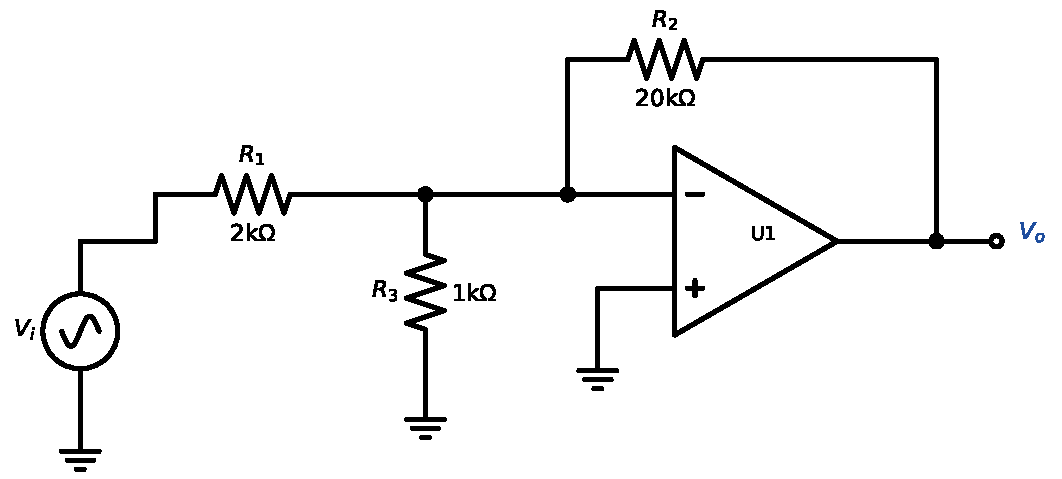
\includegraphics[width=\linewidth,height=5cm,keepaspectratio]{p15_circuit}\end{center}
\solstep{1}{Identify the sources}Independent sources: the AC input $V_i(t)$. No DC source: $V_{o,dc}=0$ and Step 2 is skipped.
\solstep{2}{DC circuit}No DC sources: $V_{o,dc}=0$.
\solstep{3}{Op-amp model}Non-ideal op-amp model (tool T5): $V_{out} = A(s)\,(V_+-V_-)$ with $A(s)=\dfrac{A_0}{1+s/\omega_b}$, $A_0=10^{5}$, $\omega_b = 2\pi\cdot10 = 62.8$\,rad/s, so the unity-gain frequency is $\omega_t = A_0\omega_b = 6.28\times 10^{6}$\,rad/s. The virtual short is \emph{not} used; only ``no current into the inputs'' is still true.

\solstep{4}{Transfer function, op-amp by op-amp}Recipe for each op-amp: write $V_+$ and $V_-$ by superposition of the block input and the op-amp output (each alone is a plain divider): $V_+ = \alpha_+V_{in}$, $V_- = \alpha_-V_{in}+\beta V_{out}$. Then $V_{out} = A(\alpha_+-\alpha_-)V_{in} - A\beta V_{out}$, i.e.\[
\frac{V_{out}}{V_{in}} = \frac{A(\alpha_+-\alpha_-)}{1+A\beta} = \frac{G}{1+\dfrac{1}{A\beta}},\qquad G = \frac{\alpha_+-\alpha_-}{\beta}\ \text{(the ideal gain)}
\]
With $A(s)$ inserted and constant $\alpha,\beta$:\[
\frac{V_{out}}{V_{in}} = G\,\frac{A_0\beta}{1+A_0\beta}\cdot\frac{1}{1+\dfrac{s}{\omega_b(1+A_0\beta)}},\qquad \omega_b(1+A_0\beta)\approx\beta\,\omega_t
\]

\textbf{Block 1 (U1).} (superposition: with $V_{o}=0$, $R_{2}$ and $R_{3}$ are in parallel from the $-$ input to ground; with $V_{i}=0$, $R_{1}$ and $R_{3}$ are. $R_{3}$ matters now, because $V_-$ is no longer forced to 0.)\begin{align*}
V_+ &= 0 \quad(\text{grounded}) \\
V_- &= \frac{R_{2}\parallel R_{3}}{R_{1}+R_{2}\parallel R_{3}}V_{i} + \frac{R_{1}\parallel R_{3}}{R_{2}+R_{1}\parallel R_{3}}V_{o}
\end{align*}
So $\alpha_+ = 0$, $\alpha_- = 0.3226$, $\beta = 0.03226$: ideal gain $G = \frac{\alpha_+-\alpha_-}{\beta} = -10$, $A_0\beta = 3230$.\[
\frac{V_{o}}{V_{i}} = -10\cdot\frac{3230}{1+3230}\cdot\frac{1}{1+\dfrac{s}{2.03\times 10^{5}}} = \frac{-9.997}{1+\dfrac{s}{2.03\times 10^{5}}}
\]
(closed-loop bandwidth $\omega_b(1+A_0\beta) = 2.03\times 10^{5}$\,rad/s, $f = 32.3 kHz$; compare $\beta\omega_t = 2.03\times 10^{5}$\,rad/s.)
So:\[
H(s) = \dfrac{-2.03\times 10^{6}}{s + 2.03\times 10^{5}}
\]

\solstep{5}{Standard (Bode-ready) form}Find the roots. Every root $s=-p$ of the denominator is a \emph{pole}, every root $s=-z$ of the numerator is a \emph{zero}; $|p|$ and $|z|$ are the corner frequencies (rad/s).
\begin{itemize}[leftmargin=*,itemsep=2pt]
\item Denominator: $s + 2.03\times 10^{5}$; $s + 2.03\times 10^{5} = 0 \Rightarrow s = -2.03\times 10^{5}$.
\end{itemize}

Factored form (leading coefficient in front):
\[
H(s) = -2.03\times 10^{6}\,\dfrac{1}{(s+2.03\times 10^{5})}
\]

Bode-ready form: rewrite every $(s+p) = p\left(1+\frac{s}{p}\right)$ and $(s+z) = z\left(1+\frac{s}{z}\right)$, and collect all constants into $K$. Then every factor except $K$ is $\approx 1$ inside the pass-band:
\[
H(s) = -10\,\dfrac{1}{1+\dfrac{s}{2\pi\cdot 32.3\mathrm{k}}},\qquad K = -10
\]

\begin{center}\renewcommand{\arraystretch}{1.35}
\begin{tabular}{cccc}
\toprule
type & $\omega_c$ (rad/s) & $f_c=\omega_c/2\pi$ & slope change \\
\midrule
pole & $2.03\times 10^{5}$ & 32.3 kHz & $-20$ dB/dec \\
\bottomrule
\end{tabular}\end{center}

\solstep{6}{Magnitude Bode plot}Below every corner, all factors are $\approx$ constant: $|H| \approx 10$ $= 20$\,dB (flat, 0 dB/dec). Then, moving right, each pole bends the line down by 20\,dB/dec and each zero bends it up by 20\,dB/dec (tool T6):
\begin{center}\renewcommand{\arraystretch}{1.35}
\begin{tabular}{lcl}
\toprule
frequency range & slope & asymptote level \\
\midrule
$f<$ 32.3 kHz & $0$ dB/dec (flat) & 20 dB at end \\
$f>$ 32.3 kHz & $-20$ dB/dec & 20 dB at start \\
\bottomrule
\end{tabular}\end{center}

The flat (pass-band) level is $20\log_{10}|K| = 20\log_{10}10 = 20$\,dB.
\begin{center}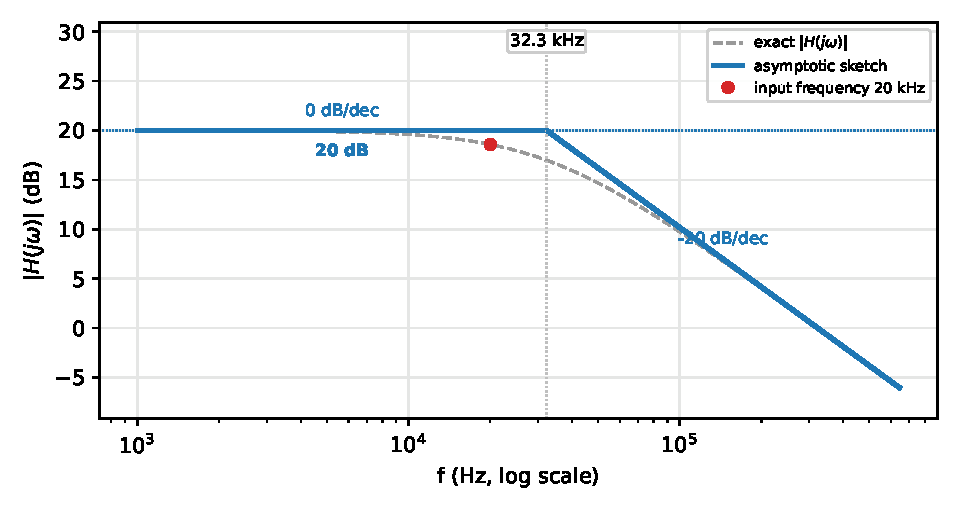
\includegraphics[width=0.78\linewidth,height=6.5cm,keepaspectratio]{p15_bode}\end{center}

{\small Blue: the straight-line sketch you are expected to draw. Dashed grey: the exact curve (about 3\,dB below the corner of an isolated pole). Red dot: the input frequency of Step 7.}
\solstep{7}{Steady-state output}The input is $V_i(t) = 0.05\cos\left(2\pi\cdot 20000\,t\right)$, so $\omega_{in} = 2\pi\cdot 20000 = 1.26\times 10^{5}$\,rad/s. Put $s=j\omega_{in}$ in each factor (tool T5): magnitudes multiply, angles add.
{\small Rules: $\left|\frac{s}{s+p}\right| = \frac{\omega}{\sqrt{\omega^2+p^2}}$, $\angle = \frac{\pi}{2}-\tan^{-1}\frac{\omega}{p}$;\quad $\left|\frac{1}{1+s/p}\right| = \frac{1}{\sqrt{1+(\omega/p)^2}}$, $\angle = -\tan^{-1}\frac{\omega}{p}$;\quad $\left|1+\frac{s}{z}\right| = \sqrt{1+(\omega/z)^2}$, $\angle = \tan^{-1}\frac{\omega}{z}$;\quad a negative $K$ adds $-\pi$.}
\begin{center}\renewcommand{\arraystretch}{1.35}
\begin{tabular}{ccc}
\toprule
factor & magnitude & angle (rad) \\
\midrule
$-10$ & $9.997$ & $-3.14$ \\
$\rule[-1.7em]{0pt}{4em}\dfrac{1}{1+\dfrac{s}{2\pi\cdot 32.3\mathrm{k}}}$ & $0.85$ & $-0.555$ \\
\textbf{total} & $\mathbf{8.497}$ (product) & $\mathbf{-3.7}$ (sum) \\
\bottomrule
\end{tabular}\end{center}

\begin{align*}
|H(j\omega_{in})| &= 8.5, \qquad \angle H(j\omega_{in}) = -3.7\ \mathrm{rad} \\
v_{o,ac}(t) &= 8.5\times 0.05\,\cos\left(2\pi\cdot 20000\,t - 3.7\right) = 0.425\,\cos\left(2\pi\cdot 20000\,t - 3.7\right)
\end{align*}

\[
\boxed{V_o(t) = 0.425\,\cos\left(2\pi\cdot 20000\,t - 3.7\right)\ \mathrm{V}}
\]

\begin{ansbox}
$H(s) = -10\,\dfrac{1}{1+\dfrac{s}{2\pi\cdot 32.3\mathrm{k}}}$\quad (corners: 32.3 kHz)\\[4pt]
$V_o(t) = 0.425\,\cos\left(2\pi\cdot 20000\,t - 3.7\right)\ \mathrm{V}$
\end{ansbox}

\newpage
\subsection*{Solution 2D.16 \hfill Hard}
\begin{center}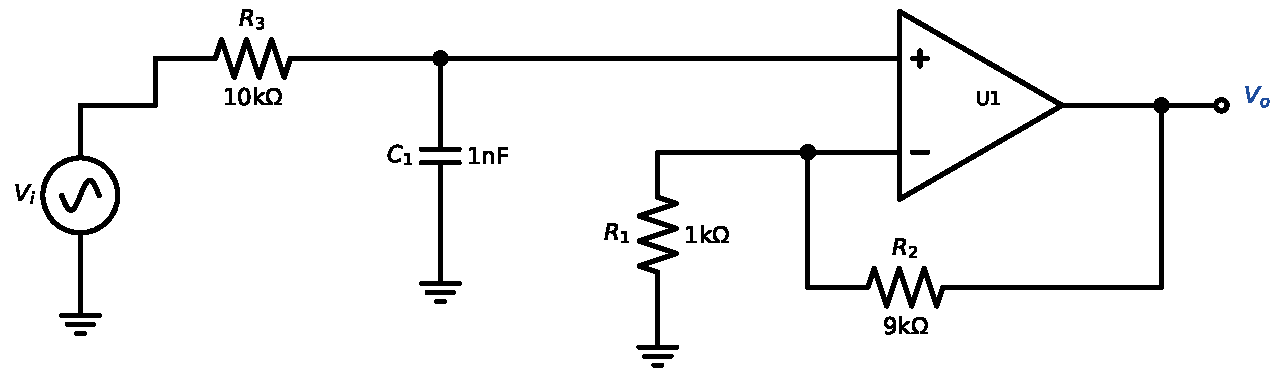
\includegraphics[width=\linewidth,height=5cm,keepaspectratio]{p16_circuit}\end{center}
\solstep{1}{Identify the sources}Independent sources: the AC input $V_i(t)$. No DC source: $V_{o,dc}=0$ and Step 2 is skipped.
\solstep{2}{DC circuit}No DC sources: $V_{o,dc}=0$.
\solstep{3}{Op-amp model}Non-ideal op-amp model (tool T5): $V_{out} = A(s)\,(V_+-V_-)$ with $A(s)=\dfrac{A_0}{1+s/\omega_b}$, $A_0=10^{5}$, $\omega_b = 2\pi\cdot10 = 62.8$\,rad/s, so the unity-gain frequency is $\omega_t = A_0\omega_b = 6.28\times 10^{6}$\,rad/s. The virtual short is \emph{not} used; only ``no current into the inputs'' is still true.

\solstep{4}{Transfer function, op-amp by op-amp}Recipe for each op-amp: write $V_+$ and $V_-$ by superposition of the block input and the op-amp output (each alone is a plain divider): $V_+ = \alpha_+V_{in}$, $V_- = \alpha_-V_{in}+\beta V_{out}$. Then $V_{out} = A(\alpha_+-\alpha_-)V_{in} - A\beta V_{out}$, i.e.\[
\frac{V_{out}}{V_{in}} = \frac{A(\alpha_+-\alpha_-)}{1+A\beta} = \frac{G}{1+\dfrac{1}{A\beta}},\qquad G = \frac{\alpha_+-\alpha_-}{\beta}\ \text{(the ideal gain)}
\]
With $A(s)$ inserted and constant $\alpha,\beta$:\[
\frac{V_{out}}{V_{in}} = G\,\frac{A_0\beta}{1+A_0\beta}\cdot\frac{1}{1+\dfrac{s}{\omega_b(1+A_0\beta)}},\qquad \omega_b(1+A_0\beta)\approx\beta\,\omega_t
\]

\textbf{Block 1 (U1).} (no current enters either input, so both are plain dividers)\begin{align*}
V_+ &= \frac{\frac{1}{sC_{1}}}{R_{3} + \frac{1}{sC_{1}}}V_{i} \\
V_- &= \frac{R_{1}}{R_{1}+R_{2}}V_{o}
\end{align*}
Here $\alpha$ and $\beta$ depend on $s$, so substitute everything and simplify:\[
\frac{V_{o}}{V_{i}} = \frac{A(\alpha_+-\alpha_-)}{1+A\beta} = \dfrac{6.28\times 10^{11}}{s^{2} + 7.28\times 10^{5}\,s + 6.28\times 10^{10}}
\]

So:\[
H(s) = \dfrac{6.28\times 10^{11}}{s^{2} + 7.28\times 10^{5}\,s + 6.28\times 10^{10}}
\]

\solstep{5}{Standard (Bode-ready) form}Find the roots. Every root $s=-p$ of the denominator is a \emph{pole}, every root $s=-z$ of the numerator is a \emph{zero}; $|p|$ and $|z|$ are the corner frequencies (rad/s).
\begin{itemize}[leftmargin=*,itemsep=2pt]
\item Denominator: $s^{2} + 7.28\times 10^{5}\,s + 6.28\times 10^{10}$; quadratic formula:\[
s = \frac{-7.28\times 10^{5} \pm \sqrt{(7.28\times 10^{5})^2 - 4(6.28\times 10^{10})}}{2} = \frac{-7.28\times 10^{5} \pm 5.28\times 10^{5}}{2} \Rightarrow s = -10^{5},\ -6.28\times 10^{5}
\]

\end{itemize}

Factored form (leading coefficient in front):
\[
H(s) = 6.28\times 10^{11}\,\dfrac{1}{(s+10^{5})(s+6.28\times 10^{5})}
\]

Bode-ready form: rewrite every $(s+p) = p\left(1+\frac{s}{p}\right)$ and $(s+z) = z\left(1+\frac{s}{z}\right)$, and collect all constants into $K$. Then every factor except $K$ is $\approx 1$ inside the pass-band:
\[
H(s) = 10\,\dfrac{1}{1+\dfrac{s}{2\pi\cdot 15.9\mathrm{k}}}\,\dfrac{1}{1+\dfrac{s}{2\pi\cdot 100\mathrm{k}}},\qquad K = 10
\]

\begin{center}\renewcommand{\arraystretch}{1.35}
\begin{tabular}{cccc}
\toprule
type & $\omega_c$ (rad/s) & $f_c=\omega_c/2\pi$ & slope change \\
\midrule
pole & $10^{5}$ & 15.9 kHz & $-20$ dB/dec \\
pole & $6.28\times 10^{5}$ & 100 kHz & $-20$ dB/dec \\
\bottomrule
\end{tabular}\end{center}

\solstep{6}{Magnitude Bode plot}Below every corner, all factors are $\approx$ constant: $|H| \approx 10$ $= 20$\,dB (flat, 0 dB/dec). Then, moving right, each pole bends the line down by 20\,dB/dec and each zero bends it up by 20\,dB/dec (tool T6):
\begin{center}\renewcommand{\arraystretch}{1.35}
\begin{tabular}{lcl}
\toprule
frequency range & slope & asymptote level \\
\midrule
$f<$ 15.9 kHz & $0$ dB/dec (flat) & 20 dB at end \\
15.9 kHz -- 100 kHz & $-20$ dB/dec & 20 dB at start, 4.03 dB at end \\
$f>$ 100 kHz & $-40$ dB/dec & 4.03 dB at start \\
\bottomrule
\end{tabular}\end{center}

The flat (pass-band) level is $20\log_{10}|K| = 20\log_{10}10 = 20$\,dB.
\begin{center}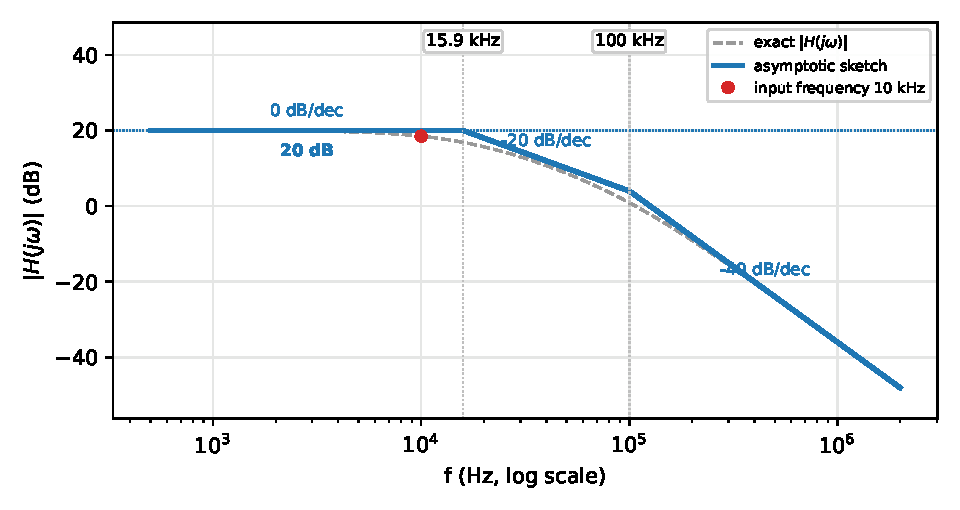
\includegraphics[width=0.78\linewidth,height=6.5cm,keepaspectratio]{p16_bode}\end{center}

{\small Blue: the straight-line sketch you are expected to draw. Dashed grey: the exact curve (about 3\,dB below the corner of an isolated pole). Red dot: the input frequency of Step 7.}
\solstep{7}{Steady-state output}The input is $V_i(t) = 0.1\sin\left(2\pi\cdot 10000\,t\right)$, so $\omega_{in} = 2\pi\cdot 10000 = 62800$\,rad/s. Put $s=j\omega_{in}$ in each factor (tool T5): magnitudes multiply, angles add.
{\small Rules: $\left|\frac{s}{s+p}\right| = \frac{\omega}{\sqrt{\omega^2+p^2}}$, $\angle = \frac{\pi}{2}-\tan^{-1}\frac{\omega}{p}$;\quad $\left|\frac{1}{1+s/p}\right| = \frac{1}{\sqrt{1+(\omega/p)^2}}$, $\angle = -\tan^{-1}\frac{\omega}{p}$;\quad $\left|1+\frac{s}{z}\right| = \sqrt{1+(\omega/z)^2}$, $\angle = \tan^{-1}\frac{\omega}{z}$;\quad a negative $K$ adds $-\pi$.}
\begin{center}\renewcommand{\arraystretch}{1.35}
\begin{tabular}{ccc}
\toprule
factor & magnitude & angle (rad) \\
\midrule
$10$ & $9.999$ & $0$ \\
$\rule[-1.7em]{0pt}{4em}\dfrac{1}{1+\dfrac{s}{2\pi\cdot 15.9\mathrm{k}}}$ & $0.8467$ & $-0.561$ \\
$\rule[-1.7em]{0pt}{4em}\dfrac{1}{1+\dfrac{s}{2\pi\cdot 100\mathrm{k}}}$ & $0.995$ & $-0.0997$ \\
\textbf{total} & $\mathbf{8.424}$ (product) & $\mathbf{-0.661}$ (sum) \\
\bottomrule
\end{tabular}\end{center}

\begin{align*}
|H(j\omega_{in})| &= 8.42, \qquad \angle H(j\omega_{in}) = -0.661\ \mathrm{rad} \\
v_{o,ac}(t) &= 8.42\times 0.1\,\sin\left(2\pi\cdot 10000\,t - 0.661\right) = 0.842\,\sin\left(2\pi\cdot 10000\,t - 0.661\right)
\end{align*}

\[
\boxed{V_o(t) = 0.842\,\sin\left(2\pi\cdot 10000\,t - 0.661\right)\ \mathrm{V}}
\]

\begin{ansbox}
$H(s) = 10\,\dfrac{1}{1+\dfrac{s}{2\pi\cdot 15.9\mathrm{k}}}\,\dfrac{1}{1+\dfrac{s}{2\pi\cdot 100\mathrm{k}}}$\quad (corners: 15.9 kHz, 100 kHz)\\[4pt]
$V_o(t) = 0.842\,\sin\left(2\pi\cdot 10000\,t - 0.661\right)\ \mathrm{V}$
\end{ansbox}

\newpage
\subsection*{Solution 2D.17 \hfill Hard}
\begin{center}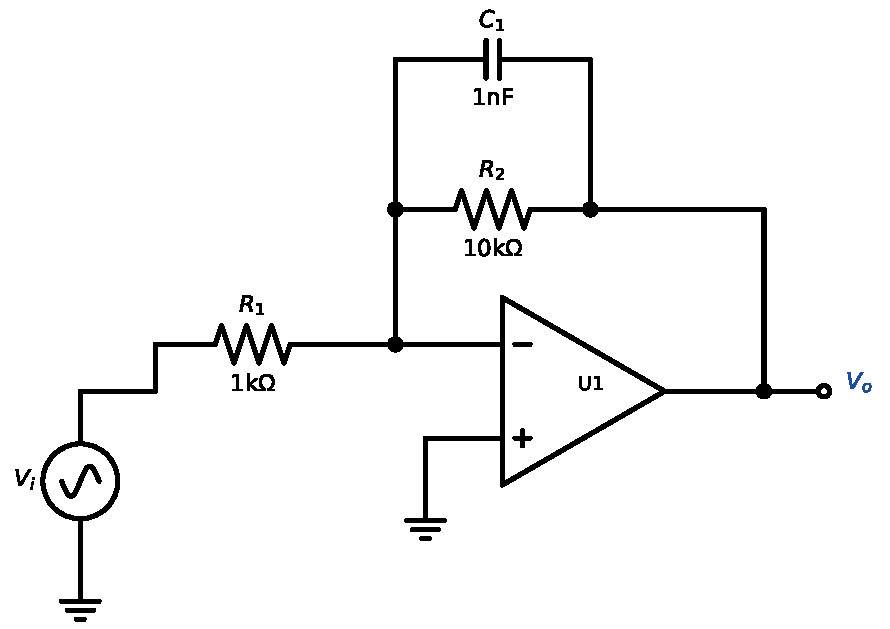
\includegraphics[width=\linewidth,height=5cm,keepaspectratio]{p17_circuit}\end{center}
\solstep{1}{Identify the sources}Independent sources: the AC input $V_i(t)$. No DC source: $V_{o,dc}=0$ and Step 2 is skipped.
\solstep{2}{DC circuit}No DC sources: $V_{o,dc}=0$.
\solstep{3}{Op-amp model}Non-ideal op-amp model (tool T5): $V_{out} = A(s)\,(V_+-V_-)$ with $A(s)=\dfrac{A_0}{1+s/\omega_b}$, $A_0=10^{5}$, $\omega_b = 2\pi\cdot10 = 62.8$\,rad/s, so the unity-gain frequency is $\omega_t = A_0\omega_b = 6.28\times 10^{6}$\,rad/s. The virtual short is \emph{not} used; only ``no current into the inputs'' is still true.

\solstep{4}{Transfer function, op-amp by op-amp}Recipe for each op-amp: write $V_+$ and $V_-$ by superposition of the block input and the op-amp output (each alone is a plain divider): $V_+ = \alpha_+V_{in}$, $V_- = \alpha_-V_{in}+\beta V_{out}$. Then $V_{out} = A(\alpha_+-\alpha_-)V_{in} - A\beta V_{out}$, i.e.\[
\frac{V_{out}}{V_{in}} = \frac{A(\alpha_+-\alpha_-)}{1+A\beta} = \frac{G}{1+\dfrac{1}{A\beta}},\qquad G = \frac{\alpha_+-\alpha_-}{\beta}\ \text{(the ideal gain)}
\]
With $A(s)$ inserted and constant $\alpha,\beta$:\[
\frac{V_{out}}{V_{in}} = G\,\frac{A_0\beta}{1+A_0\beta}\cdot\frac{1}{1+\dfrac{s}{\omega_b(1+A_0\beta)}},\qquad \omega_b(1+A_0\beta)\approx\beta\,\omega_t
\]

\textbf{Block 1 (U1).} (superposition: $V_{i}$ alone with $V_{o}=0$ gives a divider $R_{1}$--$Z_{f1}$, and vice versa)\begin{align*}
Z_{f1} &= R_{2} \parallel \frac{1}{sC_{1}} = \dfrac{10^{9}}{s + 10^{5}}
\end{align*}
\begin{align*}
V_+ &= 0 \quad(\text{grounded}) \\
V_- &= \frac{Z_{f1}}{R_{1}+Z_{f1}}V_{i} + \frac{R_{1}}{R_{1}+Z_{f1}}V_{o}
\end{align*}
Here $\alpha$ and $\beta$ depend on $s$, so substitute everything and simplify:\[
\frac{V_{o}}{V_{i}} = \frac{A(\alpha_+-\alpha_-)}{1+A\beta} = \dfrac{-6.28\times 10^{12}}{s^{2} + 7.38\times 10^{6}\,s + 6.28\times 10^{11}}
\]

So:\[
H(s) = \dfrac{-6.28\times 10^{12}}{s^{2} + 7.38\times 10^{6}\,s + 6.28\times 10^{11}}
\]

\solstep{5}{Standard (Bode-ready) form}Find the roots. Every root $s=-p$ of the denominator is a \emph{pole}, every root $s=-z$ of the numerator is a \emph{zero}; $|p|$ and $|z|$ are the corner frequencies (rad/s).
\begin{itemize}[leftmargin=*,itemsep=2pt]
\item Denominator: $s^{2} + 7.38\times 10^{6}\,s + 6.28\times 10^{11}$; quadratic formula:\[
s = \frac{-7.38\times 10^{6} \pm \sqrt{(7.38\times 10^{6})^2 - 4(6.28\times 10^{11})}}{2} = \frac{-7.38\times 10^{6} \pm 7.21\times 10^{6}}{2} \Rightarrow s = -86100,\ -7.3\times 10^{6}
\]

\end{itemize}

Factored form (leading coefficient in front):
\[
H(s) = -6.28\times 10^{12}\,\dfrac{1}{(s+86100)(s+7.3\times 10^{6})}
\]

Bode-ready form: rewrite every $(s+p) = p\left(1+\frac{s}{p}\right)$ and $(s+z) = z\left(1+\frac{s}{z}\right)$, and collect all constants into $K$. Then every factor except $K$ is $\approx 1$ inside the pass-band:
\[
H(s) = -10\,\dfrac{1}{1+\dfrac{s}{2\pi\cdot 13.7\mathrm{k}}}\,\dfrac{1}{1+\dfrac{s}{2\pi\cdot 1.16\mathrm{M}}},\qquad K = -10
\]

\begin{center}\renewcommand{\arraystretch}{1.35}
\begin{tabular}{cccc}
\toprule
type & $\omega_c$ (rad/s) & $f_c=\omega_c/2\pi$ & slope change \\
\midrule
pole & $86100$ & 13.7 kHz & $-20$ dB/dec \\
pole & $7.3\times 10^{6}$ & 1.16 MHz & $-20$ dB/dec \\
\bottomrule
\end{tabular}\end{center}

\solstep{6}{Magnitude Bode plot}Below every corner, all factors are $\approx$ constant: $|H| \approx 10$ $= 20$\,dB (flat, 0 dB/dec). Then, moving right, each pole bends the line down by 20\,dB/dec and each zero bends it up by 20\,dB/dec (tool T6):
\begin{center}\renewcommand{\arraystretch}{1.35}
\begin{tabular}{lcl}
\toprule
frequency range & slope & asymptote level \\
\midrule
$f<$ 13.7 kHz & $0$ dB/dec (flat) & 20 dB at end \\
13.7 kHz -- 1.16 MHz & $-20$ dB/dec & 20 dB at start, -18.6 dB at end \\
$f>$ 1.16 MHz & $-40$ dB/dec & -18.6 dB at start \\
\bottomrule
\end{tabular}\end{center}

The flat (pass-band) level is $20\log_{10}|K| = 20\log_{10}10 = 20$\,dB.
\begin{center}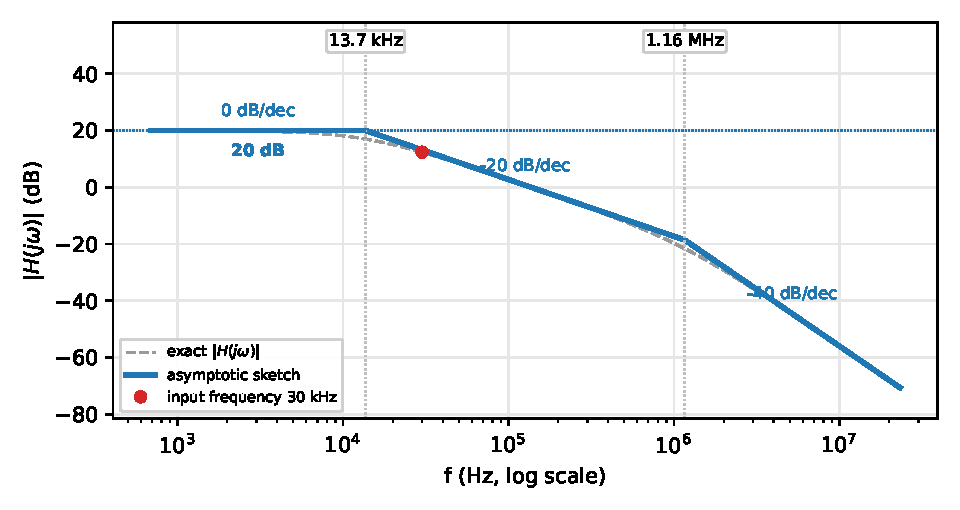
\includegraphics[width=0.78\linewidth,height=6.5cm,keepaspectratio]{p17_bode}\end{center}

{\small Blue: the straight-line sketch you are expected to draw. Dashed grey: the exact curve (about 3\,dB below the corner of an isolated pole). Red dot: the input frequency of Step 7.}
\solstep{7}{Steady-state output}The input is $V_i(t) = 0.1\sin\left(2\pi\cdot 30000\,t-\frac{\pi}{6}\right)$, so $\omega_{in} = 2\pi\cdot 30000 = 1.88\times 10^{5}$\,rad/s. Put $s=j\omega_{in}$ in each factor (tool T5): magnitudes multiply, angles add.
{\small Rules: $\left|\frac{s}{s+p}\right| = \frac{\omega}{\sqrt{\omega^2+p^2}}$, $\angle = \frac{\pi}{2}-\tan^{-1}\frac{\omega}{p}$;\quad $\left|\frac{1}{1+s/p}\right| = \frac{1}{\sqrt{1+(\omega/p)^2}}$, $\angle = -\tan^{-1}\frac{\omega}{p}$;\quad $\left|1+\frac{s}{z}\right| = \sqrt{1+(\omega/z)^2}$, $\angle = \tan^{-1}\frac{\omega}{z}$;\quad a negative $K$ adds $-\pi$.}
\begin{center}\renewcommand{\arraystretch}{1.35}
\begin{tabular}{ccc}
\toprule
factor & magnitude & angle (rad) \\
\midrule
$-10$ & $9.999$ & $-3.14$ \\
$\rule[-1.7em]{0pt}{4em}\dfrac{1}{1+\dfrac{s}{2\pi\cdot 13.7\mathrm{k}}}$ & $0.4155$ & $-1.14$ \\
$\rule[-1.7em]{0pt}{4em}\dfrac{1}{1+\dfrac{s}{2\pi\cdot 1.16\mathrm{M}}}$ & $0.9997$ & $-0.0258$ \\
\textbf{total} & $\mathbf{4.154}$ (product) & $\mathbf{-4.31}$ (sum) \\
\bottomrule
\end{tabular}\end{center}

\begin{align*}
|H(j\omega_{in})| &= 4.15, \qquad \angle H(j\omega_{in}) = -4.31\ \mathrm{rad} \\
v_{o,ac}(t) &= 4.15\times 0.1\,\sin\left(2\pi\cdot 30000\,t - 4.83\right) = 0.415\,\sin\left(2\pi\cdot 30000\,t - 4.83\right)
\end{align*}

(phase: $\theta + \angle H = -\frac{\pi}{6} + (-4.31) = -4.83$\,rad.)
\[
\boxed{V_o(t) = 0.415\,\sin\left(2\pi\cdot 30000\,t - 4.83\right)\ \mathrm{V}}
\]

\begin{ansbox}
$H(s) = -10\,\dfrac{1}{1+\dfrac{s}{2\pi\cdot 13.7\mathrm{k}}}\,\dfrac{1}{1+\dfrac{s}{2\pi\cdot 1.16\mathrm{M}}}$\quad (corners: 13.7 kHz, 1.16 MHz)\\[4pt]
$V_o(t) = 0.415\,\sin\left(2\pi\cdot 30000\,t - 4.83\right)\ \mathrm{V}$
\end{ansbox}

\newpage
\subsection*{Solution 2D.18 \hfill Hard}
\begin{center}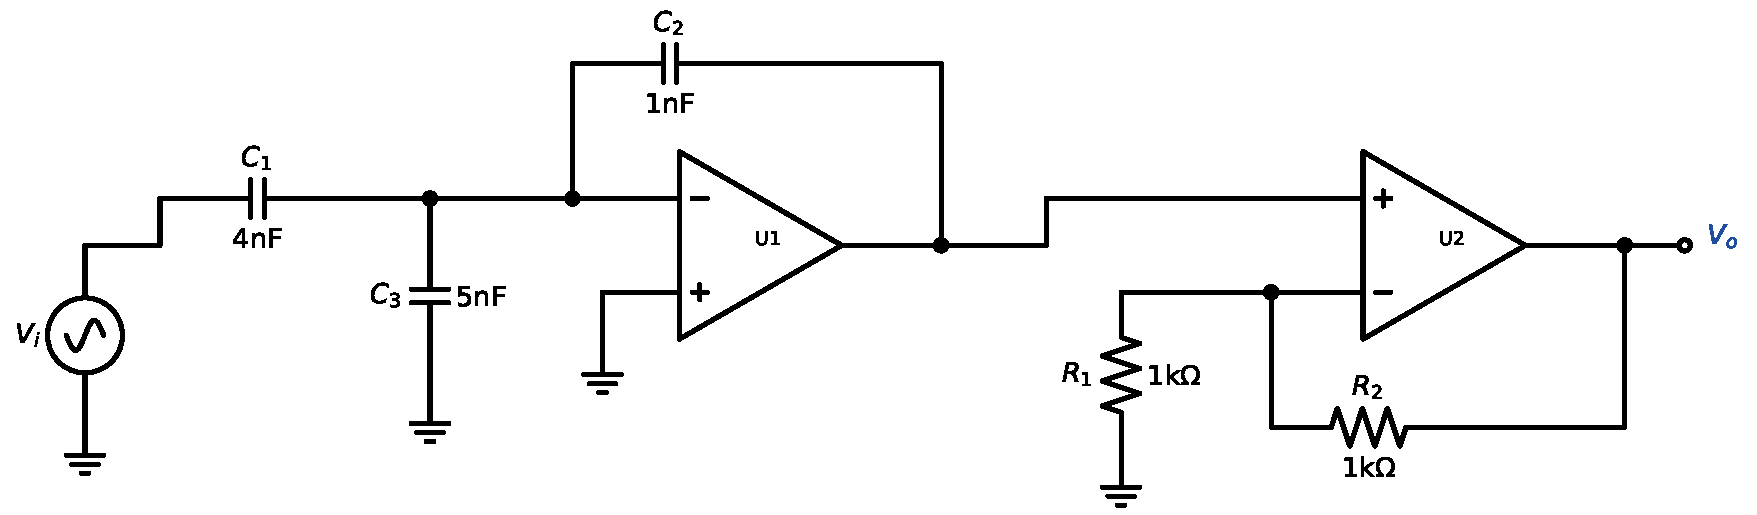
\includegraphics[width=\linewidth,height=5cm,keepaspectratio]{p18_circuit}\end{center}
\solstep{1}{Identify the sources}Independent sources: the AC input $V_i(t)$. No DC source: $V_{o,dc}=0$ and Step 2 is skipped.
\solstep{2}{DC circuit}No DC sources: $V_{o,dc}=0$.
\solstep{3}{Op-amp model}Non-ideal op-amp model (tool T5): $V_{out} = A(s)\,(V_+-V_-)$ with $A(s)=\dfrac{A_0}{1+s/\omega_b}$, $A_0=10^{5}$, $\omega_b = 2\pi\cdot10 = 62.8$\,rad/s, so the unity-gain frequency is $\omega_t = A_0\omega_b = 6.28\times 10^{6}$\,rad/s. The virtual short is \emph{not} used; only ``no current into the inputs'' is still true.

\solstep{4}{Transfer function, op-amp by op-amp}Recipe for each op-amp: write $V_+$ and $V_-$ by superposition of the block input and the op-amp output (each alone is a plain divider): $V_+ = \alpha_+V_{in}$, $V_- = \alpha_-V_{in}+\beta V_{out}$. Then $V_{out} = A(\alpha_+-\alpha_-)V_{in} - A\beta V_{out}$, i.e.\[
\frac{V_{out}}{V_{in}} = \frac{A(\alpha_+-\alpha_-)}{1+A\beta} = \frac{G}{1+\dfrac{1}{A\beta}},\qquad G = \frac{\alpha_+-\alpha_-}{\beta}\ \text{(the ideal gain)}
\]
With $A(s)$ inserted and constant $\alpha,\beta$:\[
\frac{V_{out}}{V_{in}} = G\,\frac{A_0\beta}{1+A_0\beta}\cdot\frac{1}{1+\dfrac{s}{\omega_b(1+A_0\beta)}},\qquad \omega_b(1+A_0\beta)\approx\beta\,\omega_t
\]

\textbf{Block 1 (U1).} (superposition: with $V_{o1}=0$, $\frac{1}{sC_{2}}$ and $\frac{1}{sC_{3}}$ are in parallel from the $-$ input to ground; with $V_{i}=0$, $\frac{1}{sC_{1}}$ and $\frac{1}{sC_{3}}$ are. $\frac{1}{sC_{3}}$ matters now, because $V_-$ is no longer forced to 0.)\begin{align*}
V_+ &= 0 \quad(\text{grounded}) \\
V_- &= \frac{\frac{1}{sC_{2}}\parallel \frac{1}{sC_{3}}}{\frac{1}{sC_{1}}+\frac{1}{sC_{2}}\parallel \frac{1}{sC_{3}}}V_{i} + \frac{\frac{1}{sC_{1}}\parallel \frac{1}{sC_{3}}}{\frac{1}{sC_{2}}+\frac{1}{sC_{1}}\parallel \frac{1}{sC_{3}}}V_{o1}
\end{align*}
(Only capacitors: every impedance is $\frac{1}{sC}$, so in each ratio the $s$ cancels, e.g. $\frac{1/(sC_a)}{1/(sC_a)+1/(sC_b)} = \frac{C_b}{C_a+C_b}$, and $\frac{1}{sC_a}\parallel\frac{1}{sC_b} = \frac{1}{s(C_a+C_b)}$.) So $\alpha_+ = 0$, $\alpha_- = 0.4$, $\beta = 0.1$: ideal gain $G = \frac{\alpha_+-\alpha_-}{\beta} = -4$, $A_0\beta = 10000$.\[
\frac{V_{o1}}{V_{i}} = -4\cdot\frac{10000}{1+10000}\cdot\frac{1}{1+\dfrac{s}{6.28\times 10^{5}}} = \frac{-4}{1+\dfrac{s}{6.28\times 10^{5}}}
\]
(closed-loop bandwidth $\omega_b(1+A_0\beta) = 6.28\times 10^{5}$\,rad/s, $f = 100 kHz$; compare $\beta\omega_t = 6.28\times 10^{5}$\,rad/s.)
\textbf{Block 2 (U2).} (no current enters either input, so both are plain dividers)\begin{align*}
V_+ &= V_{o1} \\
V_- &= \frac{R_{1}}{R_{1}+R_{2}}V_{o}
\end{align*}
So $\alpha_+ = 1$, $\alpha_- = 0$, $\beta = 0.5$: ideal gain $G = \frac{\alpha_+-\alpha_-}{\beta} = 2$, $A_0\beta = 50000$.\[
\frac{V_{o}}{V_{o1}} = 2\cdot\frac{50000}{1+50000}\cdot\frac{1}{1+\dfrac{s}{3.14\times 10^{6}}} = \frac{2}{1+\dfrac{s}{3.14\times 10^{6}}}
\]
(closed-loop bandwidth $\omega_b(1+A_0\beta) = 3.14\times 10^{6}$\,rad/s, $f = 500 kHz$; compare $\beta\omega_t = 3.14\times 10^{6}$\,rad/s.)
Each op-amp output is still an ideal source (it is $A(V_+-V_-)$), so the stages multiply.
Multiply the blocks and simplify:\[
H(s) = \dfrac{-1.58\times 10^{13}}{s^{2} + 3.77\times 10^{6}\,s + 1.97\times 10^{12}}
\]

\solstep{5}{Standard (Bode-ready) form}Find the roots. Every root $s=-p$ of the denominator is a \emph{pole}, every root $s=-z$ of the numerator is a \emph{zero}; $|p|$ and $|z|$ are the corner frequencies (rad/s).
\begin{itemize}[leftmargin=*,itemsep=2pt]
\item Denominator: $s^{2} + 3.77\times 10^{6}\,s + 1.97\times 10^{12}$; quadratic formula:\[
s = \frac{-3.77\times 10^{6} \pm \sqrt{(3.77\times 10^{6})^2 - 4(1.97\times 10^{12})}}{2} = \frac{-3.77\times 10^{6} \pm 2.51\times 10^{6}}{2} \Rightarrow s = -6.28\times 10^{5},\ -3.14\times 10^{6}
\]

\end{itemize}

Factored form (leading coefficient in front):
\[
H(s) = -1.58\times 10^{13}\,\dfrac{1}{(s+6.28\times 10^{5})(s+3.14\times 10^{6})}
\]

Bode-ready form: rewrite every $(s+p) = p\left(1+\frac{s}{p}\right)$ and $(s+z) = z\left(1+\frac{s}{z}\right)$, and collect all constants into $K$. Then every factor except $K$ is $\approx 1$ inside the pass-band:
\[
H(s) = -8\,\dfrac{1}{1+\dfrac{s}{2\pi\cdot 100\mathrm{k}}}\,\dfrac{1}{1+\dfrac{s}{2\pi\cdot 500\mathrm{k}}},\qquad K = -8
\]

\begin{center}\renewcommand{\arraystretch}{1.35}
\begin{tabular}{cccc}
\toprule
type & $\omega_c$ (rad/s) & $f_c=\omega_c/2\pi$ & slope change \\
\midrule
pole & $6.28\times 10^{5}$ & 100 kHz & $-20$ dB/dec \\
pole & $3.14\times 10^{6}$ & 500 kHz & $-20$ dB/dec \\
\bottomrule
\end{tabular}\end{center}

\solstep{6}{Magnitude Bode plot}Below every corner, all factors are $\approx$ constant: $|H| \approx 8$ $= 18.1$\,dB (flat, 0 dB/dec). Then, moving right, each pole bends the line down by 20\,dB/dec and each zero bends it up by 20\,dB/dec (tool T6):
\begin{center}\renewcommand{\arraystretch}{1.35}
\begin{tabular}{lcl}
\toprule
frequency range & slope & asymptote level \\
\midrule
$f<$ 100 kHz & $0$ dB/dec (flat) & 18.1 dB at end \\
100 kHz -- 500 kHz & $-20$ dB/dec & 18.1 dB at start, 4.08 dB at end \\
$f>$ 500 kHz & $-40$ dB/dec & 4.08 dB at start \\
\bottomrule
\end{tabular}\end{center}

The flat (pass-band) level is $20\log_{10}|K| = 20\log_{10}8 = 18.1$\,dB.
\begin{center}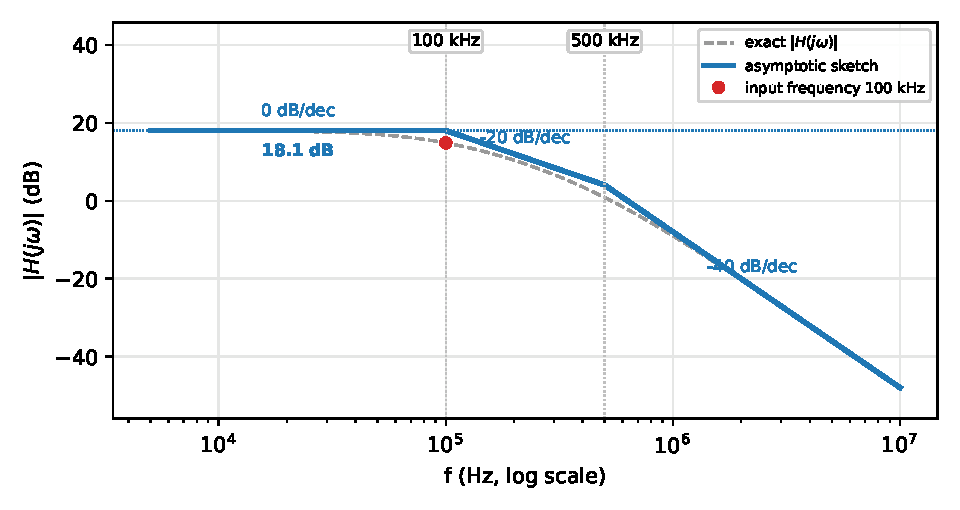
\includegraphics[width=0.78\linewidth,height=6.5cm,keepaspectratio]{p18_bode}\end{center}

{\small Blue: the straight-line sketch you are expected to draw. Dashed grey: the exact curve (about 3\,dB below the corner of an isolated pole). Red dot: the input frequency of Step 7.}
\solstep{7}{Steady-state output}The input is $V_i(t) = 0.02\sin\left(2\pi\cdot 10^{5}\,t\right)$, so $\omega_{in} = 2\pi\cdot 10^{5} = 6.28\times 10^{5}$\,rad/s. Put $s=j\omega_{in}$ in each factor (tool T5): magnitudes multiply, angles add.
{\small Rules: $\left|\frac{s}{s+p}\right| = \frac{\omega}{\sqrt{\omega^2+p^2}}$, $\angle = \frac{\pi}{2}-\tan^{-1}\frac{\omega}{p}$;\quad $\left|\frac{1}{1+s/p}\right| = \frac{1}{\sqrt{1+(\omega/p)^2}}$, $\angle = -\tan^{-1}\frac{\omega}{p}$;\quad $\left|1+\frac{s}{z}\right| = \sqrt{1+(\omega/z)^2}$, $\angle = \tan^{-1}\frac{\omega}{z}$;\quad a negative $K$ adds $-\pi$.}
\begin{center}\renewcommand{\arraystretch}{1.35}
\begin{tabular}{ccc}
\toprule
factor & magnitude & angle (rad) \\
\midrule
$-8$ & $7.999$ & $-3.14$ \\
$\rule[-1.7em]{0pt}{4em}\dfrac{1}{1+\dfrac{s}{2\pi\cdot 100\mathrm{k}}}$ & $0.7071$ & $-0.785$ \\
$\rule[-1.7em]{0pt}{4em}\dfrac{1}{1+\dfrac{s}{2\pi\cdot 500\mathrm{k}}}$ & $0.9806$ & $-0.197$ \\
\textbf{total} & $\mathbf{5.547}$ (product) & $\mathbf{-4.12}$ (sum) \\
\bottomrule
\end{tabular}\end{center}

\begin{align*}
|H(j\omega_{in})| &= 5.55, \qquad \angle H(j\omega_{in}) = -4.12\ \mathrm{rad} \\
v_{o,ac}(t) &= 5.55\times 0.02\,\sin\left(2\pi\cdot 10^{5}\,t - 4.12\right) = 0.111\,\sin\left(2\pi\cdot 10^{5}\,t - 4.12\right)
\end{align*}

\[
\boxed{V_o(t) = 0.111\,\sin\left(2\pi\cdot 10^{5}\,t - 4.12\right)\ \mathrm{V}}
\]

\begin{ansbox}
$H(s) = -8\,\dfrac{1}{1+\dfrac{s}{2\pi\cdot 100\mathrm{k}}}\,\dfrac{1}{1+\dfrac{s}{2\pi\cdot 500\mathrm{k}}}$\quad (corners: 100 kHz, 500 kHz)\\[4pt]
$V_o(t) = 0.111\,\sin\left(2\pi\cdot 10^{5}\,t - 4.12\right)\ \mathrm{V}$
\end{ansbox}

\end{document}
